\documentclass[a4paper,12pt,%
headsepline,%
numbers=noenddot,% entfernt die Punkte nach den Gliederungsziffern
]{scrreprt}

\usepackage[T1]{fontenc}
\usepackage[utf8]{inputenc}
\usepackage[ngerman]{babel}
\usepackage{setspace} 


%-----------hübsche Darstellung -------------
\usepackage{siunitx} % SI-Einheiten werden schick dargestellt
\sisetup{locale = DE} % Komma als Trenner bei Dezimalzahl erkannt

%-----------Grafiken-------------
\usepackage{graphicx} % Grafiken einbinden


%----------überprüfen------------
\usepackage{microtype}

%----------zuletzt laden---------
\usepackage[pagebackref=true]{hyperref} %







%----------eigene Befehle--------
\newcommand{\npref}[1]{\nameref{#1} (S. \pageref{#1})} 
% Überschriften
% wenn \npref{referenz} aufgerufen wird, wird automatisch eine Sequenz eingefügt: "`Name (s. X)"' zB "`Sylvan (S. 3)"'
\newcommand{\epref}[1]{\ref{#1} (S. \pageref{#1})} 
% Tabellen und Abbildungen
% wenn \epref{referenz} aufgerufen wird, wird automatisch eine Sequenz eingefügt: "`Zahl (s. X)"' zB "`3.5 (S. 3)"'





\begin{document}

\begin{titlepage}
	\centering
	\vfill
	\Large{\textbf{Stand {\today}}} \\ \bigskip
	\vfill
	\textsf{\textbf{\Huge{Wissenssammlung}}} \\ \bigskip
	\Large{\textbf{zur Übersicht der Geschichte von MMG der Ink Inc.}} \\ \bigskip
	\vfill
	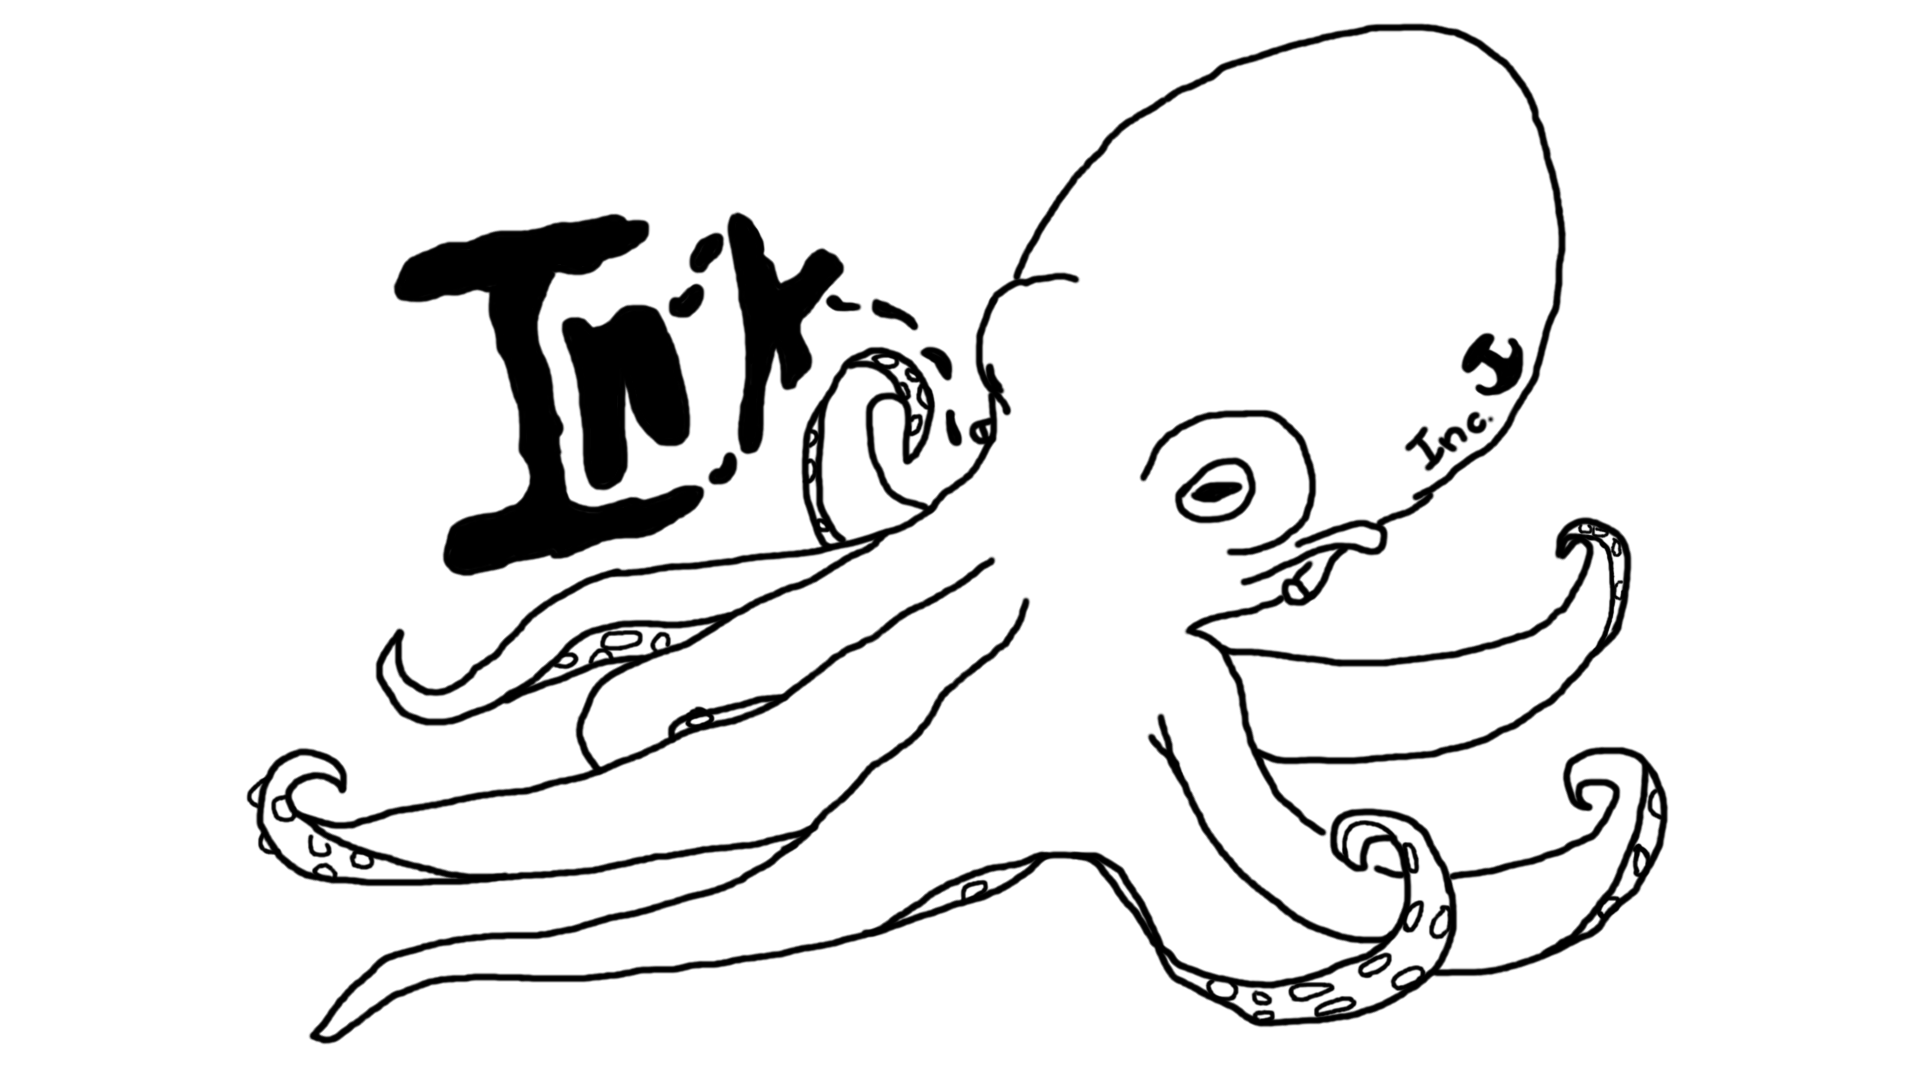
\includegraphics[width=\linewidth]{Abbildungen/logo.png} \\ \bigskip
	\vfill
	\large
	bearbeitet von\\
	Medsmiley, Thabb, Mine Schokokeks \\ \bigskip
	Concept-Art von Fossor
\end{titlepage}

\pagenumbering{Roman}
\tableofcontents
\listoffigures



%----------Inhalt-------------
\chapter*{Einleitung}
\pagenumbering{arabic}
Dieses Dokument dient zur Sammlung und Aufbewahrung allen beschlossenen Wissens bezüglich des MMG Spiels der Ink Inc. Die Lore soll einen guten Hintergrund geben, damit eine Vorstellung der Welt existiert. Damit lässt sich dann die Gesellschaft aufbauen, in der der Spieler seinen Charakter das Abenteuer erleben lässt. \\
Ebenso werden hier Mechaniken erläutert, die in das Spiel eingebaut werden sollen. \\

Nichts zu suchen haben hier detaillierte NSC- oder Questbeschreibungen. Dieses Netzwerk aus Beziehungen erfassen wir in einer eigens dafür erstellten Plattform. 

\part{Weltenbau}
\chapter{Karte \& Ökologie}
\href{http://www.weltenbau-wissen.de/sci-fi-erschaffen-fantasy-welt-erstellen-einstieg/}{Welt erstellen} \\
\href{http://www.weltenbau-wissen.de/2015/10/weltenbau-fragenkatalog-oekologie-biologie/}{Fragenkatalog} \\
\href{http://www.weltenbau-wissen.de/2015/01/weltenbau-mit-weltkarte-karte-zeichnen-tutorial/}{Weltkarte zeichnen} \\
\href{https://inkarnate.com/}{Weltenbautool}

\section{Sonnensystem}
\subsection{Welt + Zwilling}
\begin{itemize}
	\item unsere Erde ist ein zwei-Planeten System - ähnlich wie wir es haben mit Erde und Mond. Entstehung auch ähnlich, allerdings ist unser "Mond" deutlich größer: beide Planeten haben fast die gleiche Masse und natürlich praktisch die gleichen Elemente
	\item die zwei Planeten sind kleiner als die Erde. Bzw. müssen sie halt mindestens so groß sein, dass sie eine Atmosphäre halten können: \\
	Es ist ein Problem, wenn unsere Planeten zu klein sind... Man geht davon aus, dass sich das Leben auf Planeten mit unterschiedlicher Größe auch deutlich anders entwickelt hätten (Gravitation ist hier ausschlaggebend). Tatsächlich bewegen sich alle als erd-ähnlich und potenziell bewohnbar eingestuften Planeten, die wir bisher entdeckt haben zischen 0,6 und 2,5 Erdmassen und einem Radius von 0,9 bis 1,4-fachen des Erdradius. Merkur hat 0,05 Erdmassen und nur einen Drittel des Erdradius, ist also viel viel zu klein um jemals Leben wie auf der Erde entwickeln zu können, selbst wenn er in der habitablen Zone läge. Der Mars hat übrigens 0,1 Erdmassen und den 0,5 fachen Durchmesser. Einzig die Venus läge mit 0,8 Erdmassen und etwa gleichen Radius in der vielleicht gerade noch so okayen Range. Wir werden also wohl oder übel mit fast-erdgleichen Planeten arbeiten müssen, zumindest wenn wir es korrekt halten wollen.
	\item dadurch, dass sie sich so dicht beieinander befinden, erfolgte nach der Entstehung des Lebens auf einem der Planeten die Übertragung auf den anderen durch Meteroiten-Einschläge, die ihrerseits Brocken in das All hinausschießen ließen, von denen halt welche mit Leben drauf auf den anderen Planeten auftrafen (da sie so dicht beieinander sind)
	\item im Laufe der Zeit ist das Gleiche erfolgt wie bei unserem Mond: die Drehung um die eigene Achse ist so, dass sich die Planeten immer mit der gleichen Seite angucken. Und die Drehung insgesamt im Doppel-Planeten-System ist jeweils auch so, dass es einen "normalen" Tag-Nacht-Rhythmus gibt
	\item "normal" heißt hier zB gleiche Stunden am Tag wie bei uns oder etwas mehr -- aaaber die Entfernung von der Sonne und die Bahn ist so, dass das Jahr deutlich länger ist. Wir haben also deutlich längere Jahreszeiten - was uns zugute kommt, wenn man bedenkt, dass wir keinen Winter und Herbst noch einfügen wollen :smile:
\end{itemize}

\section{Welt}
\section{Kontinent}
\begin{itemize}
	\item Ein Grenzreich ist ein kleiner bis mittlerer Staat, dem es wie Kambodscha unter den Roten iwas geht -> gerade mit sich selbst beschäftigt
\end{itemize}

\subsection{Gebirgszug}
\subsection{Gigantus Wald} \label{formation:gigantus}
\begin{itemize}
	\item wie bekannt, können auch Pflanzen die ihnen innewohnende Magie nutzen. Eine Art (!!) von Bäumen haben folgendes entwickelt: sie ermöglichen mittels der Magie die Wasserversorgung der oberen Baumabschnitte gegen die Gravitation. Das Größeneinschränkende Element normaler Bäume ist damit weg. Daher konnten die Bäume extrem groß werden, bevor weitere Prozesse ihr Wachstum stoppten und hatten damit den Platz an der Sonne sicher
	\item  diese Garganten (Working title) erreichen Höhen von 500m und ähnlich wie aus dem Dschungel bekannt, bilden sich somit verschiedene vertikale Lebensbereiche
	\item der Boden ist bedeckt mit allerlei Gehölz und Sträuchern, die wenig Sonnenlicht brauchen, und ganz vorne voran riesigen Pilzen, die in Symbiose mit den riesigen Bäumen ebenfalls ein gigantisches unterirdisches Netzwerk bildeten und nun gigantische Fruchtkörper (:mushroom:  das da) ausbilden können
	\item die ersten kräftigen Äste der Garganten haben stark grüne, mit viel Chlorophyll gefüllte Blätter, die jegliches Licht, das durch die oberen Schichten kommt, aufnehmen kann. Für unsere Verhältnisse stehen die Bäume zwar ewig weit auseinander, doch auf ein normales Größenverhältnis reduziert nicht. Ihre Äste können sich an den Spitzen erreichen und bilden so mittels der Äste und den riesigen Laubblättern eine Art zweiten Boden, beginnend in 200m Höhe
	\item durch die Ausmaße der Äste sammelt sich Erde hier und dort und es wachsen normale Bäume auf dieser Ebene, allerdings nicht zu weit vom Stamm der Garganten entfernt. Ebenso finden sich hier normale Büsche etc. Schlingpflanzen ziehen sich um die dicken Äste und es bildete sich so im Laufe der Zeit in dicker "Boden" - mit unerwartete Löchern hier und da
	\item Da wir uns hier schon in der Krone der Bäume befinden, ist ab dieser zweiten Schicht ein langsamer Verlauf in den folgenden 300m: Die Baumkrone begünstigt in ihren Ausmaßen das Wachsen anderer Bäume, Sträucher, Kräuter etc, insbesondere parasitischer Lebensformen wie Schlingpflanzen und Misteln. Auch einige "normale Bäume" wachsen nicht nur auf den Erdansammlungen, sondern auch in das Holz der Äste hinein. Insgesamt bildet sich so wie eine Art Gerüst, welches aus festen "Platformen", aus festen und wackligen Wegen horizontal, vertikal und schräg, aus Bereichen lockerer Vegetation (wie Lianen) und aus "Lichtungen" (3D, nicht 2D) besteht.
	\item nach oben hin werden die Blätter der Garganten immer lichtdurchlässiger. Die untersten Blätter sind mehrere Meter dick und dunkelgrün vor Chlorophyll. Die obersten sind nur ein paar Zentimeter dick, kleiner, leicht hellgrün gefärbt und ansonsten Lichtdurchlässig. Das sorgt dafür, dass das Licht bis unten hin durchkommt und effizient genutzt werden kann, um den riesigen Baum (und seine Parasiten) zu versorgen
	\item ebenso wie die Fauna, hat sich hier auch viel Getier angesammelt und angepasst in den verschiedenen Stufen. So nisten bestimmte Vögel nur in den oberen 50m der Baumkronen. Auch ein paar Menschen fanden sich hier vor langer Zeit ein und haben sich an das Leben in den Baumkronen (von 200-350m etwa) angepasst. Es ist die Heimat der \npref{rasse:sylvan}.
	\item allerdings ist dann doch der einschränkende faktor zum einen die stabilität von holz, bevor der baum unter der eigenlast zusammenbricht, und die biegsamkeit von holz, bevor höhenwinde den baum zerbrechen. gegen letzteres könnte der baum natürlich einfach sehr dick sein. mit werten, die ich jetzt auf die schnelle für holz gefunden hab, sollte das ganze bei wenigen hundert m höhe schon instabil werden. man könnte vielleicht argumentieren, dass der baum nicht nur wasser besser transportieren kann, sondern auch mineralstoffe, um seine stabilität zu erhöhen. dann hätte man gleich ein inhärent sehr hartes holz in der welt. bei dieser höhe ist die breite auch fast egal (solange sie wenige meter überschreitet)
\end{itemize}

\section{Land}
\section{Tal}
\subsection{Teich 1}
\subsection{Teich 2}
\subsection{Großer Wald}
\subsection{Klippe am Eingang}

 
\chapter{Magie}
\section{Das Konzept der Magie}
\subsection{Was ist Magie?}
In diesem Universum ist Magie eine besondere Form der Energie und ist ein Nebenprodukt bei Energieumwandlungen.
Es entsteht also überall dort Magie, wo irgendeine Form der Energie in eine andere umgewandelt wird - was sowohl in der belebten als auch der unbelebten Natur ständig der Fall ist.
So führen z.B. Steinschläge oder Lawinen zu einem plötzlichen Auftreten einer gewissen Menge von Magie, während ein Vulkanausbruch hingegen eine ziemliche Masse an Magie produziert. 
Ja schon allein die Plattentektonik sorgt für das Vorkommen von Magie.
Da Magie eine Form der Energie ist, kann sie deshalb auch selbst wieder zurück in andere Energieformen umgewandelt werden.
Im Allgemeinen "`diffundiert"' die erzeugte Magie nämlich von ihrem Ort der Entstehung hinweg in die Umgebung, da es nichts gibt, was sie halten würde.
Dort wird sie nach und nach wieder umgewandelt.


\subsection{Anpassung der belebten Natur}
Es ist also kein Wunder, dass Magie hier auf \nameref{sec:planet} nichts besonderes ist, und dass sich das Leben dementsprechend auch entwickelte - denn insbesondere in und um Zellen erfolgt am laufenden Band die Umwandlung von Energie zwischen verschiedenen Formen.
Daher haben Zellen eine Möglichkeit entwickelt, Energie in Form von Magie zu halten und zu einem gewissen Grad anzusammeln.
Bei Eukaryoten (Pflanzen, Pilze, Tiere) ist dies eine Art Vakuole. 
Die maximal zu haltende Menge ist artabhängig und angeboren.
Ist diese Menge überschritten, so diffundiert alles Überschüssige wieder aus der Zelle in die Umwelt.
Die so gehaltene Menge an Magie wird auch als Mana oder Manapool bezeichnet.

Eine Verbildlichung lässt sich mit einer Zisterne darstellen: diese füllt sich mit dem Wasser vom Dach des Hauses, bis sie voll ist.
Danach läuft sie über und das Wasser verteilt sich in der Gegend.

Ursprünglich war dies ein Vorteil bezüglich des Überlebens der Zelle: im größten Notfall, wenn die Zelle keine Energiezufuhr jegweder Art erhält, dann kann sie ein energieintensives Notprogramm initialisieren, welches ihr die Magie als tatsächliche Energiereserve zu nutzen ermöglicht.
So kann die Zelle einen kurzen Zeitraum ohne Versorgung überbrücken.
Im Laufe der Evolution haben viele Lebewesen dann Mechanismen entwickelt, um die ihnen innewohnende Magie in ihrem Sinne auf einem intuitiven Level umzuwandeln bzw einzusetzen.
Bei Tieren kann man sich das wie eine Art zweites Nervensystem vorstellen, welches sich an den Adern entlang durch den ganzen Körper zieht und vom Rückenmark aus kontrolliert wird.
Dieses Geflecht wird aus besonderen Zellen gebildet, die selbst keine Magie speichern, sondern die Magie aus den restlichen Zellen des Körpers abziehen.
Diese gelangt somit in das Netzwerk, wo sie über das Rückenmark gezielt kontrolliert werden kann.

In welcher Weise sie die Magie kontrollieren können, ist genetisch festgelegt und hat sich evolutionär entwickelt.
Der Einsatz erfolgt im intuitiven Sinne wie ein Reflex oder eine Reaktion auf etwas, das passiert, oder unterstützt eine Handlung. 
So gibt es Pflanzen, die zur Abwehr von Fressfeinden kleine Elektroschocks verteilen, zum Anlocken von Bestäubern mit Licht spielen, oder Prädatoren, die mittels Infrarot-Magie ihre Beute ohne Probleme von der Umgebung unterscheiden können.

Jeder Mensch beherrscht die Magie auf diesem Level und zeigt sich erstmals im Bereich von 4-7 Jahren.
Im Verlauf der Differenzierungen der verschiedenen Menschenarten haben sich unterschiedliche Ausprägungen durchgesetzt oder sind erst entstanden.


\subsection{Aktive Verwendung}
Einige Lebewesen haben zudem die Fähigkeit entwickelt, die Magie aktiv in ihrem Interesse einzusetzen.
Bei Tieren bedeutet das, dass sich auch das Gehirn bei der Steuerung einschaltet.
Dabei wird sie auf ein Ziel ausgerichtet und dort werden die bestehenden Zustände geändert.
Es muss allerdings eine deutlich größere Menge an Magie eingesetzt werden, als der Vorgang bzw. die Änderung eigentlich an Energie benötigen würde.
So hat auch der Mensch schließlich festgestellt, dass er mithilfe seines Willens und Konzentration dazu in der Lage ist, diese Möglichkeiten auszubauen und zu verstärken.
Nur Personen, die sich intensiv mit ihren Fähigkeiten auseinandersetzen, viel meditieren, experimentieren und Verständnis suchen, nur diese Personen lernen, das Tauschverhältnis zu reduzieren und immer mehr zu einem halbwegs äquivalenten Austausch zu kommen.
Das führt dazu, dass sie mit dem ihnen angeborenen Manapool mehr und stärkere Dinge bewirken können.
Ihre einzigen Grenzen sind dabei durch ihre Gene, ihre Vorstellungskraft, ihre Konzentrationsfähigkeit und den magischen Widerstand anderer Lebewesen gesetzt. 
\\ \\
Es gibt ein paar Prokaryoten, die sich die Magie als tatsächliche dauerhafte Energiequelle erschlossen haben und sie ständig direkt zur Herstellung von ATP (Adenosintriphosphat = "`Energie der Zelle"') nutzen können.
Bisher ist noch kein Fall von Symbiose oder gar Endosymbiose ähnlich wie mit den Mitos (\textalpha-Proteobakterien $\rightarrow$ Mitochondrien) oder Chloros (Cyanobakterien $\rightarrow$ Chloroplasten) bekannt, aus dem höher entwickelte Lebewesen herausgekommen sind, da dies vor nicht allzu langer Zeit (in Zeiträumen der Evolution) entstand.


\subsection{Natürlicher magischer Widerstand}
Ist es im Allgemeinen nicht schwer, den eigenen Körper und die Umgebung zu beeinflussen, so ist das Verändern von Zuständen in anderen Körpern ein ganz anderes Thema.
Höher entwickelte Lebewesen, die ein Verständnis für den eigenen Körper oder sogar ein Ich-Bewusstsein erlangt haben, besitzen dadurch einen Art natürlichen magischen Widerstand gegen Änderungen, die in ihrem Körper erfolgen sollen. 
Dieser ist umso stärker, je ausgereifter das Bewusstsein ist.
Das führt dazu, dass nur wirklich mächtige und studierte Individuen es schaffen, diese Barriere zu überwinden und Magie innerhalb solcher Körper zu wirken.



\section{Magie-Kontrolle}
\paragraph{Hintergrund}
Magie kann eingesetzt werden, um bestimmte physikalische oder chemische Prozesse zu verändern - in einem gewissen Rahmen, der genetisch vererbt wurde.
Somit bedeutet die Beherrschung einer Magie-Art eigentlich, dass das Wesen dazu fähig ist, die Magie kontrolliert in diese bestimmte Art Energie umzusetzen.
Welche Arten bisher schon entstehen zeigt die kategorisierte Übersicht in Abb. \ref{fig:magiearten-uebersicht}.

\begin{figure}[htb]
	\centering
	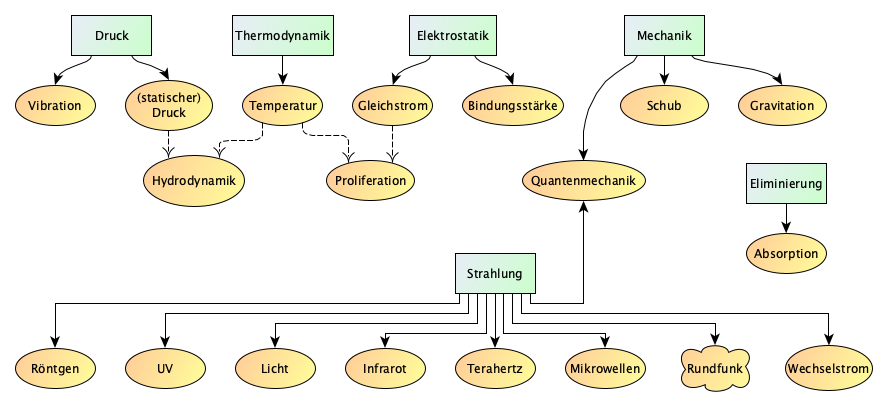
\includegraphics[width=\linewidth]{Abbildungen/Weltenbau/Magie/Magiearten-Uebersicht}
	\caption[Übersicht der Arten der Magiekontrolle]{\textbf{Alle bekannten Arten der Kontrolle über Magie in der Übersicht.} \\ 
	Verwandte Arten sind durch ihre Kategorisierung und ihre Verbindung über Pfeile gekennzeichnet.}
	\label{fig:magiearten-uebersicht}
\end{figure}


\paragraph{Stufen der Kontrolle}
Bei den folgenden verschiedenen Arten der Magie-Kontrolle, auch Magiearten genannt, ist dargestellt, wie die intuitive Nutzung dieser Eigenschaft aussieht oder wie Begabte mit ihr umgehen können.
Meisterliche Magier erreichen noch ganz andere Level. 
In der Regel sind sie schon in hohem Alter und haben sich ihr Leben lang mit der Verbesserung, dem Lernen und Ausprobieren beschäftigt, weshalb es nur wenige gibt, die so weit kommen. 
Neben der Intensivierung und Verbesserung vorheriger Zauber gelingt ihnen auch eine Manipulation ganz anderer Art: 
Sie können die natürliche Resistenz des Körpers (siehe oben) umgehen.


\paragraph{Magie-Arten}
Die Informationen über die Verbreitung der Magiearten unter den Lebewesen und ihrer Bekanntheit in \nameref{sec:land} finden sich einerseits bei jeder Art und andererseits in Tab. \ref{tab:magie-verbreitung} zur Übersicht.
Für eine genaue Auflistung der Magiearten in \nameref{sec:land} siehe Tab. \ref{tab:landmagie}.

Die Anordnung der Magiearten ist alphabetisch, um einen schnellen Zugriff zu ermöglichen.

\begin{table}[htb]
	\centering
	\caption{\textbf{Verbreitung der Magiearten unter den Lebewesen allgemein und unter den Menschenarten auf dem Kontinent.}}
	\label{tab:magie-verbreitung}
	\begin{threeparttable}[\linewidth]
		\begin{tabular}{l|ccc}
			\toprule
			\textbf{Art} & \textbf{Eukaryoten} & \textbf{Hominini} & \textbf{Mensch} \\
		    \midrule
			\nameref{magie:absorption}  & - & - & (x)  \\
			\nameref{magie:bindung} & X & \nameref{rasse:sylvan} & -  \\
			(statischer) \nameref{magie:druck} & X & X & X  \\
			\nameref{magie:gleichstrom}  & X & X & \nameref{sec:mc-diplomatin}  \\
			\nameref{magie:gravitation} & - & - & - \\ \midrule[0.1px]
			\nameref{magie:hydrodynamik} & X & X &\\
			\nameref{magie:infrarot} & X & X & X \\
			\nameref{magie:licht}  & X & X & \nameref{sec:mc-spionin}  \\
			\nameref{magie:mikrowelle} & X & X & X \\
			\nameref{magie:proliferation} & X & X & X \\ \midrule[0.1px]
			\nameref{magie:quantenmechanik} & X & ? & - \\
			\nameref{magie:roentgen} & X & - & - \\
			\nameref{magie:rundfunk} & X & - & - \\
			\nameref{magie:schub} & X & X & \nameref{sec:mc-diplomatin} \\
			\nameref{magie:temperatur} & X & X & \nameref{sec:mc-soldat} \\ \midrule[0.1px]
			\nameref{magie:terahertz} & X & X & X \\
			\nameref{magie:uv} & X & \nameref{rasse:ferus} & - \\
			\nameref{magie:vibration} & X & \nameref{rasse:zwerg}, \nameref{rasse:unda} & -  \\
			\nameref{magie:wechselstrom} & X & X & X \\
			\bottomrule
		\end{tabular}
	\end{threeparttable}
\end{table}



\subsection{Absorption oder Nullmagie}\label{magie:absorption}
Diese Art der Kontrolle sorgt für einen ständigen Entzug von Magie aus der Umwelt, da der Magie-Speicher in den Zellen (z.B. von Menschen) beschädigt ist oder fehlt. 
Dadurch können die Zellen gesammelte Magie nicht mehr halten und versuchen kontinuierlich weiter, Magie aufzunehmen.

\subsubsection{Verbreitung und Bedeutung im Spiel}
Zu Beginn des Spiels beherrschen nur Mikroorganismen diese Fähigkeit. Sie ist daher anfangs vollkommen unbekannt. 
Am Ende des Spiels wird eine neue Art Mensch geschaffen, die diese Fähigkeit ebenso beherrscht.

\subsubsection{Intuitive Nutzung}
Die Bakterien nutzen es als Energiequelle mittels eines speziellen Zellorgans. 
Es lässt sich ähnlich vorstellen wie die Nutzung von Sonnenenergie mittels Chloroplasten oder chemischer Energie mittels Mitochondrien. 

Die Menschen werden durch das heftige Absorbieren sämtlicher Magie relativ unbeeinflussbar durch Magie, die direkt auf sie gewirkt wird oder auf das, was sie berühren. 
Sie sind jedoch unfähig, selbst Magie zu wirken.

\subsubsection{Erlernbare Steigerungen}
Es wird sehr lange dauern, bis die Menschen begreifen, dass auch dies eine Möglichkeit zur Steigerung bietet.
\begin{outline}
	\1 Magie, die gerade auf die erweiterte Umgebung gewirkt wird, wird annulliert.
	\1 Es ist ein verlängertes Fasten möglich, da der Körper auf die Umgebungsmagie zurückgreift.
	\1 ...
\end{outline}

\subsubsection{Meisterliche Beherrschung} 
\begin{outline}
	\1 Aktives Absorbieren von Magie aus Lebewesen, was diese daran hindert, ihre Magie einsetzen zu können.
	\1 ...
\end{outline}
Zurück zu Tab. \ref{tab:magie-verbreitung}.



\subsection{Bindungsstärke}\label{magie:bindung}
Mittels dieser Fähigkeit lassen sich Atombindungen stärken oder schwächen, wodurch ein Verhärtungs- oder Erweichungseffekt hervorgerufen wird. 
Allerdings führt eine höhere Bindungsenergie auch zu einer kleineren räumlichen Nähe der Atome. 
Da die Magie der Bindungsstärke erst unter Einfluss der \nameref{magie:druck}-Magie entstand, wird dabei gleichzeitig ein starker negativer (Verhärtung) oder positiver (Erweichung) Druck von außen appliziert. 
Dadurch verkleinert oder vergrößert sich das veränderte Material nicht plötzlich um den gleichen Faktor.

Da in Gasen zwischen den einzelnen Bestandteilen keine Atombindungen vorliegen, lässt sich dies hauptsächlich nur bei Festkörpern und ggf. bei Flüssigkeiten anwenden.

\subsubsection{Verbreitung}
Dies ist vor allem unter Pflanzen, wie auch den Bäumen aus dem \nameref{sec:gigantuswald}, verbreitet.
Bei den Hominini können nur Sylvan auf diese Weise Magie kontrollieren.

\subsubsection{Bedeutung im Spiel}
Derzeit ist keine Bedeutung im Spiel geplant. 
Eventuell durch andere Lebewesen oder sollte man die Sylvan (ggf. auch durch ein DLC) tatsächlich treffen können.

\subsubsection{Intuitive Nutzung}
Intuitiv nutzen Lebewesen dies, um den eigenen Körper zu stärken, wenn es um eingehende Verletzungen geht, zB. beim Kampf oder beim Fallen (Schockabsorption). 
Einige machen ihren Körper dadurch zeitweise etwas beweglicher, um durch kleinere Spalte hindurch zu passen.
Dies ist auch anwendbar auf Oberflächen, die direkt berührt werden. 
Auf diese Art sorgen zB. die Sylvan dafür, dass dünnere Blätter und Äste unter ihrem Gewicht nicht zerbrechen.

\subsubsection{Erlernbare Steigerungen}
\begin{outline}
	\1 Zerreißen von Dingen.
	\1 Bewusstes Weglassen des Drucks von außen führt zu einer Volumenänderung des betroffenen Bereichs. 
	Dies bedeutet einerseits starkes Anwachsen oder extremes Verkleinern. 
	Das Gewicht ändert sich dabei nicht. 
	Die Weiterleitung von Signalen an Nervenzellen u.ä. ist allerdings auch beeinträchtigt: wenn größer, dann langsamer, wenn kleiner, dann schneller.
	\1 ...
\end{outline}

\subsubsection{Meisterliche Beherrschung} 
\begin{outline}
	\1 Erschaffen temporärer Löcher im Körper, durch die zB etwas durch kann, bevor dies wieder rückgängig gemacht wird.
	\1 Anwendung in Alchemie: Stoffe werden dazu gebracht Verbindungen einzugehen, die normalerweise eine zu hohe Energiebarriere haben.
	\1 ...
\end{outline}
Zurück zu Tab. \ref{tab:magie-verbreitung}.



\subsection{Druck}\label{magie:druck}
Diese Eigenschaft erlaubt die Kontrolle über den lokalen, statischen Druck. 
Im Sinne der aufzubringenden Energie ist Druck daher auf Gase, Flüssigkeiten und weiche Feststoffe bzw. welche, die sich wie Flüssigkeiten verhalten (Sand, Erde, ...), begrenzt.

Es existiert die präzisere Unterform \nameref{magie:vibration}, sowie als Neuentwicklung die Magie der \nameref{magie:bindung}.

\paragraph{Unterscheidung zum Schub}
Es gibt mehrere Punkte, in denen sich Druck grundlegend von Schub unterscheidet.
So wird Druck zur Bewegung von außen auf einen Körper gewirkt, während Schub an einem Punkt im Körper ansetzt und sich der Rest des Körpers durch die stoffliche Beschaffenheit mitbewegt.
Der Druck von außen beeinflusst aber auch alle anderen Objekte in der Umgebung, da er nicht nur in eine Richtung wirkt.
Dabei kann er unbeabsichtigt auch zerstörerisch auf gewählte Strukturen wirken, denn um die nötige Energie aufzubringen, muss der Druck in der Regel recht schnell gewirkt werden.

Im Gegenzug lassen sich mit Druck Dinge an einem Punkt halten oder zerquetschen, was mit Schub nicht so gut möglich ist.

\subsubsection{Verbreitung}
Ähnlich wie bei der thermischen Energie ist diese Form recht weit verbreitet. 
Die homininen Arten beherrschen diese Kontrolle. 

In \nameref{sec:land} ist die Magieform allerdings nicht ganz so häufig andere anzutreffen. 

\subsubsection{Bedeutung im Spiel}
Bisher ist keine besondere Bedeutung vorgesehen.

\subsubsection{Intuitive Nutzung}
Einige Lebewesen können somit in einer Art Reaktion Gefahren, die zu nah an sie herankommen, von sich wegschubsen bzw. sich selbst wegdrücken, ohne etwas zu berühren. 
Andere nutzen dies, um das Kauen harter Pflanzen und Früchte zu unterstützen und somit zusätzliche Nahrungsquellen zu erschließen.
Manche Vogel- und Fischarten können durch eine feinere Perzeption von Druck am Körper nun Druckgradienten besser erkennen und nutzen.

\subsubsection{Erlernbare Steigerungen}
\begin{outline}
	\1 Es wird Druck auf andere Dinge angewendet, womit sie entweder auseinander gerissen oder zerquetscht werden.
	\1 Gegenstände oder Lebewesen werden kontrolliert an Ort und Stelle gehalten.
	\1 Gegenstände oder Lebewesen werden durch die Gegend gedrückt.
	\1 Einkommender Druck kann abgefangen und auf eine größere Fläche verteilt werden: zuerst nur bei größerflächigen Dingen wie Steinen oder Stöcke. 
	Später auch gegen Waffen, die genau so was ausnutzen: Klingenwaffen. 
	Dadurch wird weniger Schaden genommen.
	\1 Formung weicher Objekte durch Druckanwendung, z.B. heißes Metall beim Schmieden, heißes Glas beim Glasblasen, Bretter biegen für den Schiffsbau, etc.
	\1 ...
\end{outline}

\subsubsection{Meisterliche Beherrschung} 
\begin{outline}
	\1 Den Druck im Kopf erhöhen bis er platzt.
	\1 Den Blutdruck plötzlich extrem absenken, so dass das Gegenüber bewusstlos zusammenbricht. 
	\1 Den Druck in der Umgebung so stark beeinflussen, dass sich dadurch das Wetter ändern kann. 
	Damit lassen sich zB. Regenwolken lenken.
	\1 ...
\end{outline}
Zurück zu Tab. \ref{tab:magie-verbreitung}.



\subsection{Gleichstrom}\label{magie:gleichstrom}
Mit dieser Eigenschaft lassen sich elektrische Ladungen beeinflussen und verschieben.
So kann eine große Potentialdifferenz zwischen zwei Orten aufgebaut werden, die sich ab einem bestimmten Punkt selbst ausgleicht: meist in Form eines Blitzes.
Weiterhin ist es mit dieser Beeinflussung möglich, die nötige Ladung so zu verschieben, dass Redox-Reaktionen ablaufen: Funken fliegen, Feuer entsteht, Explosionen krachen.

Der Unterschied in der Gefährlichkeit für Lebewesen ist beim \nameref{magie:wechselstrom} dargestellt.

\subsubsection{Verbreitung}
Dies ist weit unter Tieren und insbesondere Pflanzen verbreitet. 
Auch die Hominini besitzen diese Fähigkeit, allerdings ist ihnen Elektrizität im weiteren (heutigen) Sinne noch kein Begriff, weshalb das bisherige Ausnutzen und Ausbauen dieser Kontrolle recht schlecht erforscht ist.

\subsubsection{Bedeutung im Spiel}
Die \npref{sec:mc-diplomatin} erhält den Zugriff auf diese Fähigkeit nach ihrem Schlüsselerlebnis. 

\subsubsection{Intuitive Nutzung}
Da die Weiterleitung von elektrischen Impulsen an Nerven dem Prinzip des Gleichstroms folgt, ist dies bei den Besitzern beschleunigt.
Daraus folgt eine etwas schnellere körperliche Reaktion auf Situationen.
Zudem schweben die anwendenden Lebewesen durch einen Blitzeinschlag nicht in Lebensgefahr.  

\subsubsection{Erlernbare Steigerungen}
Die Hominini kennen Strom hauptsächlich von Blitzen und versuchen deshalb, sie nachzuahmen. 
Diese Anwendungsform ist allerdings sehr ineffizient, da sie dabei versuchen, all ihre Magie auf einmal zu entladen. 
Das führt dazu, dass Menschen höchstens kleine Funken zustande kriegen, ehe sie bessere Kontrolle und Selbstbeherrschung lernen.
Anfangs beschränkt es sich daher im Endeffekt meist auf das Auslösen von Reaktionen.
\begin{outline}
	\1 Es kann ein Potentialunterschied zwischen zwei Punkten hergestellt werden, der zu einem Ausgleich der Energie über einen Blitz führt.
	Die Stärke des Blitzes und die Entfernung der Punkte a) zueinander und b) vom Anwender sind von dessen Fähigkeiten abhängig.
	Zu Beginn wird nur eine Übertragung zwischen sich und einem anderen Punkt möglich sein.
	\1 Entflammbare Objekte können angezündet werden, da der Reaktion zwischen Objekt und dem Sauerstoff aus der Luft der nötige Schubs zum Start gegeben wird.
	\1 Mit der nötigen Energiemenge lässt sich das Wasser in der Luft in Sauerstoff und Wasserstoff spalten und somit Knallgas herstellen.
	Kommt das Knallgas mit einem Funken in Kontakt, führt das zu einer sofortigen explosiven Revers-Reaktion, bei der sich die beiden wieder zu Wasser verbinden.
	Einflüsse, Stellschrauben u.ä. für die Erweiterung dieses Skills zur Anwendung im Spiel finden sich \zB auf \href{https://de.wikipedia.org/wiki/Knallgas}{Wikipedia}.
	\1 ...
\end{outline}

\subsubsection{Meisterliche Beherrschung} 
\begin{outline}
	\1 Der elektrische Signalfluss an Nervenzellen lässt sich stören, womit zum Beispiel eine Reaktion des Gegenübers verhindert wird. 
	Das ist allerdings recht unpräzise, da die Funktionsweise des Körpers noch nicht so weit bekannt ist. 
	Durch das Spüren der Ströme konnten allerdings einige Erkenntnisse gewonnen werden. 
	So lässt sich \zB sämtlicher elektrischer Fluss in einzelne Gliedmaßen ausschalten, wodurch diese nicht mehr bewegt werden können.
	\1 Ebenso kann man das Gehirn von jemanden lahm legen und ihn damit effektiv töten.
	\1 Das Herz wird von einem Nervenknoten, dem Sinus, kontrolliert. 
	Bei Herzstillstand kann man es wieder zum schlagen bringen, indem man diesem Knoten einen elektrischen Impuls gibt, damit das Herz wieder zu arbeiten beginnt (siehe auch \href{https://de.wikipedia.org/wiki/Defibrillator}{Defibrillator}).
	\1 Schnelleres Denken.
	\1 Eigene Reflexe verbessern (ggf. schwieriger zu kontrollieren als das Stören gegnerischer Reflexe, da man nicht in Zuckungen am Boden enden will)
	\1 ...
\end{outline}
Zurück zu Tab. \ref{tab:magie-verbreitung}.



\subsection{Gravitation}\label{magie:gravitation}
Diese Magieform erlaubt eine Beeinflussung der Gravitation.

\subsubsection{Verbreitung}
Dies ist eine äußerst seltene Magieform, die von keinen bisher bekannten Tieren oder Pflanzen verwendet wird.
Auch unter den Hominini ist sie nicht verbreitet.

\subsubsection{Bedeutung im Spiel}
Derzeit keine Bedeutung im Spiel.

\subsubsection{Intuitive Nutzung}
Intuitiv kann man damit die Auswirkung der Gravitation auf sich selbst reduzieren, was u.a. zu deutlich höheren und weiteren, aber auch unpräziseren Sprüngen führt.
Auf der anderen Seite lässt sich damit effektiv auch das eigene Gewicht erhöhen, wodurch beispielsweise die Standfestigkeit im Sturm erhöht ist.

\subsubsection{Erlernbare Steigerungen}
\begin{outline}
	\1 Durch Erhöhen der Gravitation in einem Bereich lassen sich dort andere Lebewesen festhalten.
	\1 Anders herum kann man so auch befreundeten Wesen beim Springen oder ähnlichem helfen.
	\1 ...
\end{outline}

\subsubsection{Meisterliche Beherrschung} 
\begin{outline}
	\1 Durch Wirken von Gravitation im Körper von anderen, lässt sich damit ihr Innenleben zerreißen und verzerren, weshalb sie wahrscheinlich einen sehr schmerzhaften Tod sterben.
	\1 ...
\end{outline}
Zurück zu Tab. \ref{tab:magie-verbreitung}.



\subsection{Hydrodynamik}\label{magie:hydrodynamik}
Hier geht es  um Strömungen von Flüssigkeiten und Gasen.
Am verständlichsten sollte dies sein, wenn von Wind oder Wasserströmen gesprochen wird.
Die Kontrolle über Hydrodynamik entsteht aus einem Mix der Fähigkeiten von \nameref{magie:druck} und \nameref{magie:temperatur}, da sie so erzeugt werden kann.

\subsubsection{Verbreitung}
An sich ist dies eine durchaus verbreitete Magieart unter den Lebewesen.
In \nameref{sec:land} ist es eine eher seltenere Art, die sich nur bei Zusammentreffen eines Allels von Druck und eines von Temperatur ergibt.

\subsubsection{Bedeutung im Spiel}
Bisher ist keine besondere Bedeutung vorgesehen.

\subsubsection{Intuitive Nutzung}
Lebewesen können damit direkt um sich herum Wind erzeugen oder diesen negieren und sind daher von stürmischen Auswirkungen meist weniger betroffen.
Ebenso kann damit der eigene Geruch etwas zerstäubt werden, wodurch Beutetiere sich besser verstecken und Raubtiere ihre Beute nicht zu früh warnen.
Manche Vögel erzeugen schwache Winde um sich herum, um ihren Flug zu unterstützen und schneller fliegen bzw. leichter steuern zu können. 
Analoges gilt für manche Fische mit Wasser.

Menschen lassen dabei auch bei Windstille diesen gerne mal mit ihren Haaren oder der Kleidung spielen.

\subsubsection{Erlernbare Steigerungen}
\begin{outline}
	\1 Das Erzeugen kleiner Windhosen bzw. Staubteufel bzw. Verwirbelungen im Wasser.
	\1 Ein wenig "`Wasserbändigen"'.
	\1 Das Putzen von staubigen oder anders trocken-dreckigen Oberflächen.
	\1 Transport von Objekten durch Luftströme.
	\1 ...
\end{outline}

\subsubsection{Meisterliche Beherrschung} 
\begin{outline}
	\1 "`Blutbändigen"'.
	\1 Erzeugen von Wirbelstürmen.
	\1 ...
\end{outline}
Zurück zu Tab. \ref{tab:magie-verbreitung}.



\subsection{Infrarot}\label{magie:infrarot}
Infrarot-Strahlung ermöglicht das Sehen von Temperatur. 
Dies ist bereits in Tieren natürlich entstanden, doch einige nutzen für den gleichen Zweck die Magie.

\subsubsection{Verbreitung}
Nur Tiere haben diese Fähigkeit entwickelt, auch ein paar Menschenstämme in extremen Temperaturgebieten.

\subsubsection{Bedeutung im Spiel}
Derzeit keine Bedeutung im Spiel geplant außer über Tiere.

\subsubsection{Intuitive Nutzung}
Tiere auf der Jagd, der Lauer oder beim Wachdienst nutzen eine regelmäßige Überprüfung der Umgebung mittels Infrarotstrahlung, um die wärmeren Körper ihrer Ziele zu sehen.

Menschen können Wärmesignaturen als eine Art sechsten Sinn fühlen: das kann beispielsweise bei der Verfolgung von Spuren nützlich sein.

\subsubsection{Erlernbare Steigerungen}
\begin{outline}
	\1 In besonders kalten Gegenden hat es zu einem gegenseitigen Wettrennen zwischen Jäger und Beute geführt, bei der der Jäger die Beute mittels dieser Sicht aufspüren will, während diese damit die Abgabe ihrer Körperwärme überdeckt.
	\1 Das Erzeugen von "`falschen"' Wärmebildern, indem an anderen Orten Infrarotstrahlung erzeugt wird.
	So kann \zB ein Jäger auf die falsche Fährte geführt werden.
	\1 Mittels Erzeugen der Strahlung lässt sich die Temperatur ein wenig heben - allerdings nicht annähernd wie bei anderen Temperatur beeinflussenden Fähigkeiten .
	\1 ...
\end{outline}

\subsubsection{Meisterliche Beherrschung} 
\begin{outline}
	\1 ...
\end{outline}
Zurück zu Tab. \ref{tab:magie-verbreitung}.



\subsection{Licht} \label{magie:licht}
Diese Eigenschaft ermöglicht die Kontrolle von Licht bzw. dessen Abwesenheit.
Mit "`Licht"' ist hier als die für Menschen sichtbare elektromagnetische Strahlung gemeint.

\subsubsection{Verbreitung}
Eine recht weit verbreitete Kontrollfähigkeit unter diversen Lebewesen. 
Unter den Menschen in \nameref{sec:land} ist es eine recht weit verbreitete Magieart.

\subsubsection{Bedeutung im Spiel}
Die \npref{sec:mc-spionin} beherrscht diese Eigenschaft. 

\subsubsection{Intuitive Nutzung}
Viele Lebewesen verwenden dies zur Attraktion von anderen Lebewesen, sei es um diese zu nutzen oder als Beute.
Einerseits Licht, insbesondere bei Nacht, andererseits Illusionen um zu täuschen. \\
Man munkelt auch von einer Tierart, die sich so gut an die Umwelt anpassen, dass sie von ihrer Beute nicht entdeckt wird, bis es zu spät ist. 

Menschen nutzen dies besonders, um sich selbst attraktiver zu machen, können aber kein Licht selbst erzeugen.

\subsubsection{Erlernbare Steigerungen}
\begin{outline}
	\1 Das Erzeugen von Licht.
	\1 Mit hellem Licht lassen sich Gegner blenden oder gar erblinden.
	\1 Illusionen dienen zur Unterhaltung oder Ablenkung.
	\1 Mittels Illusionen kann man sich dem Hintergrund anpassen, wodurch man deutlich schlechter zu sehen ist.
	\1 Verbesserte Sicht bzw. weitere Sicht durch Fokussierung und Krümmung/Beugung von Lichtwegen.
	\1 ...
\end{outline}

\subsubsection{Meisterliche Beherrschung} 
\begin{outline}
	\1 Wahre Meister des Fachs können das Licht so geschickt manipulieren, dass sie einem unaufmerksamen Auge gar als unsichtbar scheinen können.
	\1 Die Kontrolle über die An- oder Abwesenheit von Licht in einem gewissen Bereich.
	\1 Feuererzeugung durch Lichtbündelung (wie mit einer Linse), allerdings langsam und daher eher für Lagerfeuer und Kerzen oä. geeignet.
	\1 Die verbesserte Sicht kann zum Blick um Ecken herum ausgebaut werden.
	\1 ...
\end{outline}
Zurück zu Tab. \ref{tab:magie-verbreitung}.



\subsection{Mikrowellen}\label{magie:mikrowelle}
Mit Mikrowellen lässt sich Wasser erhitzen und abkühlen, denn diese treffen genau die Eigenfrequenz des Wassers.
Das gilt demnach für alles, was Wassermoleküle enthält.
Weiterhin ermöglichen Mikrowellen ein Radarsystem.

\subsubsection{Verbreitung}
Vor allem bei Tieren, aber auch den Menschen in \nameref{sec:land} tritt dies auf.
Bei ihnen beherrschen Leute, in denen sich die Gene für Licht und Wechselstrom mischen, die Kontrolle über Mikrowellen.
Durch ein Crossing-Over-Event entstand auch ein eigenes Allel.

\subsubsection{Bedeutung im Spiel}
Bisher keine besondere Bedeutung im Spiel geplant.

\subsubsection{Intuitive Nutzung}
Viele Tiere mit dieser Eigenschaft haben parallel ein Radarsystem entwickelt.
Die Sensoren befinden sich mit bei den Ohren.
Das erlaubt Herdentieren oder Rudeln, sich auch über weitere Strecken hinweg zu lokalisieren, wiederzufinden oder in Bezug auf Beute zu wissen, in welche Richtung ihr noch niemand auflauert.

Ansonsten halten sich Lebewesen damit warm oder kühl, je nachdem wie die Umstände es erfordern (siehe auch \nameref{magie:temperatur} dazu).

\subsubsection{Erlernbare Steigerungen}
\begin{outline}
	\1 Erhitzung von Wasser und Essen ohne Feuer. Manche Nahrung wird erst dadurch essbar!
	\1 ...
\end{outline}

\subsubsection{Meisterliche Beherrschung} 
\begin{outline}
	\1 ...
\end{outline}
Zurück zu Tab. \ref{tab:magie-verbreitung}.



\subsection{Proliferation}\label{magie:proliferation}
Diese Eigenschaft ist eher chemischer Natur und erlaubt die Beeinflussung der Reaktionsgeschwindigkeit.
Aus diesem Grunde leitet sie sich auch von der \nameref{magie:temperatur} und dem \nameref{magie:gleichstrom} ab.
Ersteres hat direkten Einfluss auf die Geschwindigkeit: bei erhöhter Temperatur laufen Reaktionen schneller ab, da sich Teilchen schneller bewegen.
Der Gleichstrom dient als Katalysator und senkt die Energiebarriere die dem Start der Reaktion entgegensteht.
Folgen von beschleunigten Reaktionen finden sich dann auch bei den Zellen wieder: schnelleres Wachstum führt zum Beispiel zu einem schnelleren Lebenszyklus oder zur beschleunigten Reparatur von Schäden - auch im gesamten Gewebe.

\subsubsection{Verbreitung}
Wenige Pflanzen- und Tierarten sind dieser Fähigkeit mächtig. 
Unter den Hominini haben nur die Menschen dies entwickelt und auch bei ihnen ist es eine seltenere Gabe. 
Denn diese Fähigkeit leitet sich zwar von den recht häufig verbreiteten Arten Temperatur und Gleichstrom ab, doch die Fortpflanzung dieser Menschen ist eingeschränkt.
Zwar leben diese Menschen länger als ihre Verwandten, abhängig von der Intensität ihrer Begabung sogar bis zu \SI{200}{\percent} der durchschnittlichen Lebensdauer, allerdings kommt mit dieser Fähigkeit ein ungünstiger Nachteil:
sie sind fast unfähig, sich mit ihren Artangehörigen zu vermehren, da ihre Keimzellen "`nicht auf gleicher Geschwindigkeit laufen"'.
Das führt dazu, dass sich die Wahrscheinlichkeit für ein Kind drastisch verringert je nachdem wie begabt der Anwender und wie ausgebaut seine Fähigkeiten sind.

\subsubsection{Bedeutung im Spiel}
Nur sehr wenig Individuen im Land haben diese Kontrollform geerbt.
Insbesondere begabte Menschen, die zur aktiven Anwendung außerhalb des eigenen Körpers fähig sind, bleiben Einzelbeispiele.
Diese sind daher hochgeschätzte Mitglieder des Ordens und erfreuen sich bester Umstände.

Es heißt, es liegt ein solcher Magier irgendwo in einer Art Winterschlaf und er wird aufwachen, wenn die Welt ihn wieder benötigt (Ref: wie die Sage zu König Barbarossa? Ggf. unter Märchen und Quests ausfeilen). %todo

\subsubsection{Intuitive Nutzung}
Da Reparatur und Heilung schneller ablaufen, sich der Körper ansonsten aber "`ruhiger verhält"', verläuft der Alterungsprozess langsamer.

\subsubsection{Erlernbare Steigerungen}
\begin{outline}
	\1 Erweitern der gesteigerten Reaktionen auf die nahe Umwelt: Pflanzen wachsen und reifen schneller.
	Bei manchen fähigen Nutzern führt das dazu, dass sie sich besonders gerne mit schönen Pflanzen umgeben, welche stark blühen und gut gedeihen.
	Sie sind dann gerne mal in ihrem kleinen paradiesischen Garten anzutreffen, der vielen normalen Bürgern wie ein Stück des Himmels vorkommt.
	\1 Zudem kann dies zur Heilung anderer eingesetzt werden, wenn diese ihre natürliche Resistenz senken.
	Diese ist durch eine bestimmte Droge umgehbar, welche allerdings auch zusätzliche Belastung auf den Körper auswirkt. %todo ein schöner Ansatzpunkt für Folter und den Geheimdienst
	Das führt dazu, dass manche schwere Verletzungen nicht geheilt werden können, weil schon die Einnahme der Droge den Körper überstrapaziert.
	\1 ...
\end{outline}

\subsubsection{Meisterliche Beherrschung} 
Nur extrem wenige Menschen haben es geschafft, diese Stufe zu erreichen.
Sie sind daher geliebte und gefürchtete Individuen.
\begin{outline}
	\1 Das plötzliche starke Altern des Gegenübers.
	\1 Krebserzeugung.
	\1 Bisher noch unentdeckt ist eine passive Auswirkung von solch mächtigen Magiern: eine verlangsamte Alterung von Lebewesen im näheren Umfeld des Anwenders.
	Dies kommt natürlich auf lange Sicht nur bei häufiger Nähe zustande.
	\1 ...
\end{outline}
Zurück zu Tab. \ref{tab:magie-verbreitung}.



\subsection{Quantenmechanik}\label{magie:quantenmechanik}
Dies ist eine experimentelle Magieform, die wahrscheinlich keinem normalen Lebewesen zur Verfügung steht.
Ein wenig ist das die Form, die am meisten an die klassische OP-Magie mit Teleportation, Verdopplung etc. heranreicht.
Demzufolge braucht sie allerdings auch die meiste Energie - und zwar in so gigantischen Ausmaßen, dass sie teilweise nicht annähernd vernünftig zu erklären wäre.
So bräuchte die Teleportation eines Menschen schon etwa die Energiemenge einer ganzen Galaxie...

\subsubsection{Bedeutung im Spiel}
Derzeit keine Bedeutung im Spiel.

\subsubsection{Ausnutzen der Quantenmechanik}
\begin{outline}
	\1 Welle-Teilchen-Dualismus
		\2 Teilchen können sich auch wie Wellen verhalten und deshalb mit sich selbst interferieren.
		\2 Interpretation: es lassen sich einige Eigenschaften des eigenen Körpers verbessern, während sich dafür andere Verschlechtern.
		Also ein Buff zum Preise eines Debuffs.
	\1 Tunnelrate
		\2 Ein Teilchen befindet sich nur an seinem Platz, weil ihm die Energie fehlt, an einem anderen zu sein.
		\2 Interpretation: Teleportation.
	\1 Superposition
		\2 Teilchen können in mehreren Zuständen gleichzeitig existieren.
		\2 Interpretation: Duplikation von Dingen, ggf. erneute Verschmelzung nach bestimmter Zeit.
\end{outline}
Zurück zu Tab. \ref{tab:magie-verbreitung}.



\subsection{Röntgen}\label{magie:roentgen}
Röntgenstrahlung erlaubt es, tief in organisches Material hineinzusehen. 

\subsubsection{Verbreitung}
Einige Tiere beherrschen diese Fähigkeit. \\
Keine Verbreitung unter den Hominini.

\subsubsection{Bedeutung im Spiel}
Derzeit keine Bedeutung im Spiel.

\subsubsection{Intuitive Nutzung}
Gerade Jäger, die ihre Beute unter Deckung wie Bäumen und Büschen suchen, nutzen kurze blitzartige Momente der Röntgenstrahlung, um ihre Beute zu lokalisieren.
Da diese Strahlung sehr energieintensiv ist, ist eine häufige Anwendung mit dem normalen Pool an Mana nicht möglich.
\\ \\
Zurück zu Tab. \ref{tab:magie-verbreitung}.



\subsection{Rundfunk}\label{magie:rundfunk}
Diese Wellenlänge wird heutzutage zum Rundfunk genutzt.
Uns ist nichts eingefallen, wie man dies als Fähigkeit für eine nicht-technologisierte Welt einsetzen könnte.
Denn den Wesen einfach einen (detaillierten) Interpreter und Sender wie bei unseren Radiostationen in den Kopf zu packen, erschien uns unlogisch.
Da diese Frequenzen aber mitten drin unter den anderen genutzten liegt, ist eine Evolution dieser Fähigkeit äußerst wahrscheinlich.
Daher behalten wir sie uns als Option drin, insbesondere für eine spätere Nutzung im entsprechenden Zeitalter.

Sollte jemand sich mit der Thematik des Rundfunks besser auskennen und doch dafür plädieren (und es damit als eine Art Telepathie einsetzen wollen), dann bitte zur Diskussion melden.

\subsubsection{Verbreitung}
Keine Verbreitung unter den Lebewesen.

\subsubsection{Bedeutung im Spiel}
Derzeit keine Bedeutung im Spiel.

\subsubsection{Intuitive Nutzung}
Manche Insekten haben darüber eine besondere Art von Schwarmintelligenz aufgebaut.
\\ \\
Zurück zu Tab. \ref{tab:magie-verbreitung}.



\subsection{Schub}\label{magie:schub}
Schub steht für die mechanische Energie, die auf etwas appliziert werden kann.
Es geht also um Bewegung bzw. das Aufwenden der Energie, die für die jeweilige Bewegung nötig wäre.
Dabei wird jedoch immer ein Punkt verschoben, mit dem sich alles Verbundene mitbewegt.
In seiner Bewegung kann der gesamte Körper natürlich Anderes anstoßen oder beeinflussen.
Das führt dazu, dass das Bewegen von Gasen, Flüssigkeiten und Feststoffen, die sich wie letztere verhalten (Sand, Erde, ...), nicht wirklich möglich ist.

\paragraph{Unterscheidung zu \nameref{magie:druck}} 
Es gibt mehrere Punkte, in denen sich Schub von Druck abgrenzt. 
So wird Druck nicht im zu bewegenden Körper, sondern von außen drauf gewirkt.
Dabei ist der Druck von außen nicht in eine Richtung konzentriert sondern wirkt von seinem Punkt aus in alle Richtungen -- also auch auf weitere Objekte, die nichts mit dem Zielobjekt zu tun haben müssen.
In der Bewegung von Objekten ist also Schub die zuverlässige präzise Variante.

Beim Thema Anheben hat Druck den Nachteil, dass er physikalisch bereits an Grenzen stoßen oder zerstörerisch auf die gewählte Struktur wirken kann, während Schub nichts dergleichen hervorruft.
Das kommt daher, dass sich Luft unter dem Objekt befinden muss, die ausreichend ausgedehnt wird, damit dadurch das Objekt angehoben wird.
Ist es zu schwer, so kann es sein, dass der Druck in der Luft nicht so weit erhöht werden kann.
Da der erzeugte Druck recht schnell (um nicht zu sagen explosiv) die gewünschte Stärke erreichen muss, damit er sich nicht in die Umgebung verteilt, kann es sein, dass er eher den Gegenstand beschädigt, anstatt ihn zu bewegen.

Anders herum hat der Schub das Nachsehen, wenn es um Zerquetschen oder Ähnliches geht: dazu müssen hier zusätzliche Objekte auf das Ziel geschoben werden.
Mit Druck sind keine weiteren Dinge nötig.

\subsubsection{Verbreitung}
Ähnlich wie die Temperatur eine alte und weit verbreitete Fähigkeit unter den Lebewesen.
In \nameref{sec:land} ist es eine der wenn nicht sogar die häufigste Magiearten.

\subsubsection{Bedeutung im Spiel}
Die \nameref{sec:mc-diplomatin} beherrscht dies als ihre primäre Fähigkeit.

\subsubsection{Intuitive Nutzung}
Diese Anwender können den Schub auf ihre eigenen Körper wirken.
Dadurch sind etwas weitere Sprünge möglich.
Zudem können sie vor dem Auftreffen einen gegensätzlichen Schub auf sich wirken, wodurch ihre Einschlagkraft am Zielort reduziert ist.
Das führt dazu, dass sie \zB aus leicht größeren Höhen fallen können, bevor sie körperliche Schäden erhalten.
Die Puffermenge ist natürlich weiterhin abhängig von dem verfügbaren Manapool.

\subsubsection{Erlernbare Steigerungen}
\begin{outline}
	\1 Der intuitive Nutzen in gesteigerter aktiver Form.
	\1 Eine leichte Steigerungsform, die daher auch unter der Bevölkerung oft gesehen wird, ist das kleine Schieben von Last auf die Art, dass das Anheben leichter gelingt.
	\1 Levitation
	\1 Telekinese
	\1 Anstoßen von \zB (Geröll-)Lawinen.
	\1 Stärkeres Werfen von Geschossen wie Steine, Speere und andere Waffen (vgl. Kugelstoßen).
	\1 ...
\end{outline}

\subsubsection{Meisterliche Beherrschung} 
\begin{outline}
	\1 Herumschieben von anderen Personen.
	\1 Auseinanderreißen von anderen Personen, indem in den Gliedmaßen gegensätzliche Schübe appliziert werden.
	\1 ...
\end{outline}
Zurück zu Tab. \ref{tab:magie-verbreitung}.



\subsection{Temperatur}\label{magie:temperatur}
Diese Eigenschaft erlaubt die Kontrolle über die thermische Energie der Umgebung, sowohl das Erhitzen als auch das Abkühlen.

\subsubsection{Verbreitung}
Diese Manipulation der thermischen Energie ist uralt und daher weit verbreitet unter allen Arten von Lebewesen; 
Somit auch unter den homininen Arten. 
In \nameref{sec:land} ist es eine der am weitesten verbreiteten Arten unter der Bevölkerung, wobei allerdings die Magie der Mikrowellen und Infrarot-Strahlung auf intuitivem Level häufig damit verwechselt werden.

\subsubsection{Bedeutung im Spiel}
Diese Magiekontrolle beherrscht der \npref{sec:mc-soldat}.

\subsubsection{Intuitive Nutzung}
Diese Lebewesen haben weniger Temperaturprobleme, da sie den Temperaturaustausch mit der Umgebung reduzieren können.

Einige wenige Tiere nutzen dieses Konzept auch zur Jagd, sowohl an Land als auch im Wasser, wo sie die Luft oder das Wasser stark erhitzen oder extrem abkühlen und damit für Verbrennungen oder Erfrierungen sorgen.

\subsubsection{Erlernbare Steigerungen}
Zuerst Beispiele für die Erhitzung:
\begin{outline}
	\1 Das Erhitzen von Gegenständen abseits vom eigenen Körper, insbesondere sehr gut wärmeleitende Materialien wie Metall. Dies wird zB. im Kampf ausgenutzt, um die Waffe oder die Rüstung des Gegners zu heiß zum Halten/Tragen werden zu lassen.
	\1 Das Entzünden entflammbarer Objekte.
	\1 Das Erschaffen kleiner Mengen glühender Hitze, die weggeworfen werden kann. 
	Beim Aufprall entzünden sich die vor Ort befindlichen Materialien. 
	\1 Wandförmige Bereiche von Luft werden so stark erhitzt, dass alles, was sie berührt, schmilzt oder brennt.
	\1 ...
\end{outline}

Nun Beispiele für das Abkühlen:
\begin{outline}
	\1 Das Metall am Körper des Gegenübers erkalten lassen. Das kann zu Verbrennungen führen.
	\1 Feuchte Körperteile lassen sich an gefrorenen Gegenständen, insbesondere metallischen, anfrieren.
	\1 Flüssigkeiten auf dem Boden (idR Wasser) lassen sich gefrieren, womit Glatteis erzeugt wird.
	\1 Feuer lassen sich durch einen gegensätzlichen Effekt löschen.
	\1 Der Blutfluss offener Wunden lässt sich durch Abkühlung verringern.
	\1 ...
\end{outline}

\subsubsection{Meisterliche Beherrschung} 
\begin{outline}
	\1 Das Blut/der Körper des Gegners kann zum Kochen gebracht werden.
	\1 Körperteile des Gegners können erfroren werden.
	\1 ...
\end{outline}
Zurück zu Tab. \ref{tab:magie-verbreitung}.



\subsection{Terahertz}\label{magie:terahertz}
Mittels Terahertz-Strahlung lässt sich wenige Zentimeter in weiches bzw. organisches Gewebe blicken, ohne Strahlungsschäden zu riskieren.
Diese Wellenlänge wird allerdings schon von Wasser absorbiert (und damit auch von allem, was eine höhere Dichte hat).
Das erklärt die geringe Reichweite und Unschädlichkeit.

\subsubsection{Verbreitung}
Diese Art ist gerade unter den intelligenteren Tieren verbreitet, aufgrund ihres guten intuitiven Nutzens.

Die Menschen in \nameref{sec:land} kennen diese Art bisher nicht, da sie sich erst vor zwei bis drei Generationen bei einer mittelständigen Familie entwickelt hat.
Sie ist daher Objekt der Forschung.

\subsubsection{Bedeutung im Spiel}
Es wird eine Questreihe zur Entdeckung und Erforschung dieser neuen Magieart geben.

\subsubsection{Intuitive Nutzung}
Diese Fähigkeit ermöglicht es, sehr schnell Parasiten zu finden oder sich der genaueren Natur einer Verletzung gewahr zu werden.

\subsubsection{Erlernbare Steigerungen}
\begin{outline}
	\1 Material-/Probenanalyse zum einen in Handwerksberufen und zum anderen in der Alchemie und Medizin (\zB Salben, Kräuter, Gifte, etc.).
	\1 Aktives Einsetzen der Sicht, \zB zur Diagnose oder zum Erkennen, ob jemand Waffen unter seinen textilen Klamotten trägt.
	\1 ...
\end{outline}

\subsubsection{Meisterliche Beherrschung} 
\begin{outline}
	\1 ...
\end{outline}
Zurück zu Tab. \ref{tab:magie-verbreitung}.



\subsection{UV}\label{magie:uv}
Es gibt Tiere, die bereits im UV-Spektrum sehen können, ohne über Magie zu verfügen. 
Darunter fällt die Biene.

\subsubsection{Verbreitung}
Gerade Pflanzen nutzen dies, um attraktiver für Bestäuber wirken zu können. \\
Die \nameref{rasse:ferus} nutzen dies, um auch unter der Erde Vitamin~D herstellen zu können.

\subsubsection{Bedeutung im Spiel}
Derzeit keine Bedeutung im Spiel.

\subsubsection{Intuitive Nutzung}
Tiere nutzen das \zB anstatt der normalen Sicht oder ähnlich wie Bienen.

Die \nameref{rasse:ferus} hingegen erzeugen immer wieder kleine Mengen UV-Strahlung in ihrer Haut, wodurch sie auch unter der Erde dazu in der Lage sind, das nötige Vitamin~D herzustellen.

\subsubsection{Erlernbare Steigerungen}
\begin{outline}
	\1 ...
\end{outline}

\subsubsection{Meisterliche Beherrschung} 
\begin{outline}
	\1 ...
\end{outline}
Zurück zu Tab. \ref{tab:magie-verbreitung}.



\subsection{Vibration}\label{magie:vibration}
Diese Fähigkeit ist eine Weiterentwicklung der \nameref{magie:druck} im Sinne einer präziseren Manipulation.\\
Der Körper ist dazu in der Lage, verschieden-frequentige Vibrationen zu erzeugen. 
Häufig ging daher auch eine Evolution von feineren Sinnesorganen zur Rezeption dieser damit einher.

\subsubsection{Verbreitung}
Manche Lebewesen kontrollieren Magie auf diese Art, darunter auch die \nameref{rasse:zwerg} und \nameref{rasse:unda} der homininen Arten. Die Menschen beherrschen diese Verwendung der Magie nicht und da eine Reproduktion mit den anderen Arten nach der ersten Generation in einer Sackgasse steckt, bleibt ihnen nur die Erforschung.

\subsubsection{Bedeutung im Spiel}
Bedeutung findet sich hier keine weitere für die Menschen des Landes, nur in der Forschung. 
Bei den paar Zwergen, die unter den Menschen leben, sieht das natürlich anders aus.

\subsubsection{Intuitive Nutzung}
Diese Lebewesen nehmen Geräusche besser und in einer größeren Bandbreite wahr, bis hin zu einer Art Echolot-Technik. 
Allerdings können sie ihre Wahrnehmung dabei willentlich verschärfen oder abstumpfen. 
Ebenso können sie schon feinere Schwingungen über die Druckrezeptoren der Haut und Haare spüren und all diese Schwingungen auch aussenden.

Hominine nutzen das zur Kommunikation oder Orientierung in der Dunkelheit. 

\subsubsection{Erlernbare Steigerungen}
\begin{outline}
	\1 Die Wahrnehmung der Umgebung verstärkt sich extrem, teilweise werden keine Augen mehr benötigt um Dinge um sich herum zu lokalisieren. 
	\1 Die Vibration wird zu einer Art kontrollierten Sprengung oder Zerstörung von (harten) Materialien genutzt.
	\1 ...
\end{outline}

\subsubsection{Meisterliche Beherrschung} 
\begin{outline}
	\1 Von gut bekannten Dingen oder Lebewesen kennen Meister des Faches die ihnen eigenen Schwingungen bzw. Reaktion auf solche. 
	Daher können sie solche auch über weite Entfernung aufspüren.
	\1 Das Erzeugen von so lauten Geräuschen, dass sie kilometerweit zu hören sind. 
	Das kann in nächster Nähe natürlich zu Gehörschäden führen.
	\1 Gezielte Übertragung von Geräuschen über weite Entfernung, z.B. zur Kommunikation mit dem Rudel. \\ 
	Variante A: Erzeugung vor Ort und gerichtete (punktgenaue) Übertragung (auf einer Linie) zum Zielort. \\
	Variante B: Erzeugung vor Ort und Übertragung, die nicht auf direkter Linie liegt, indem die Ausbreitung des Schalls entsprechend gesteuert wird.
	Variante C: Erzeugung beim Zielort.
	\1 Knochen des Gegenübers zum Zerbröseln bringen.
	\1 ...
\end{outline}
Zurück zu Tab. \ref{tab:magie-verbreitung}.



\subsection{Wechselstrom}\label{magie:wechselstrom}
Beim Wechselstrom wird die Polung in regelmäßiger Wiederholung umgekehrt, wodurch der Strom im \textit{zeitlichen} Mittel null ist - faktisch durchlaufen aber die abwechselnden Wellen das Objekt.
Das kann zur Erhitzung führen - oder ein metallisches Objekt magnetisieren.

\paragraph{Unterschied zum Gleichstrom}
Der Wechselstrom ist im Vergleich zum \nameref{magie:gleichstrom} eine Form von Strahlung und für Lebewesen gefährlicher:
die Gefahr besteht nämlich zu einem wichtigen Teil in dem Stören der Erregungsleitung am Herzen.
In einer ganz bestimmten Phase dieser Leitung am Herzen ist der Rhythmus angreifbar und bei zusätzlicher Erregung von außen kann es zur ungeordneten Erregung, dem sogenannten Kammerflimmern, kommen $\rightarrow$ es kann kein Blut mehr gepumpt werden.
Dieses kleine Fenster wird vom Wechselstrom aufgrund des schnellen Wechsels der Polarität mit deutlich höherer Wahrscheinlichkeit getroffen.
Die Folgen hängen allerdings von weiteren Faktoren ab, wobei die geschilderten Folgen alle von trockener Haut ausgehen und einem Impuls, welcher nicht direkt auf das Herz gerichtet appliziert wird:
\begin{outline}
	\1 \textit{Die Zeitdauer:} Ist der Stromimpuls zu kurz, um Nervenzellen zu erregen, bleibt es ungefährlich.
	Ein kurzes Zappen tötet keinen.
	\1 \textit{Der Weg durch den Körper:} Am gefährlichsten ist der Weg durch alle lebenswichtigen Organe.
	Ebenso relevant ist die Nähe zum Herzen!
	Dieses ist besonders anfällig und kann zielgerichtet schon mit viel weniger ausgeschaltet werden.
	\1 \textit{Die Stromstärke:} Während eine geringe Stromdichte vielleicht auf der Zunge wahrnehmbar ist, führt die nächste Intensitätsstufe bereits zur Kontraktion der Fingermuskeln, der Blutdruck steigt und es kann für Kinder schon tödlich sein. 
	Im nächsten Schritt käme es zur Bewusstlosigkeit, Arrhythmie und stärkeren Blutdrucksteigerungen.
	Die vorletzte Stufe führt schließlich zum Atem- und Kreislaufstillstand durch Kammerflimmern bzw. Asystolie (aka Herzstillstand).
	Schließlich sorgt eine sehr hohe Stromstärke an Ein- und Austrittsstellen für Verbrennungen.
\end{outline}

\subsubsection{Verbreitung}
Dies ist weit unter Tieren und insbesondere Pflanzen verbreitet. 
Doch auch die Hominini besitzen diese Fähigkeit, allerdings ist ihnen Elektrizität oder im weiteren Sinne noch kein Begriff, weshalb das Ausbauen und Ausnutzen dieser Kontrolle recht schlecht ist.

\subsubsection{Bedeutung im Spiel}
Die \npref{sec:mc-diplomatin} hat diese Eigenschaft von Beginn an... oder?

\subsubsection{Intuitive Nutzung}
Die meisten Lebewesen nutzen kleine Schockstöße zur Abwehr von Räubern und Fraßfeinden. 
Es gibt einige Pflanzen in besonders kargen Gegenden, die gelernt haben, dies als eine Art Metalldetektor einzusetzen, um wichtige Nährstoffe im Boden zu finden.

\subsubsection{Erlernbare Steigerungen}
\begin{outline}
	\1 Metallische (magnetische) Gegenstände von entsprechender Größe sind frei bewegbar.
	\1 Metalle werden (ent-)magnetisiert.
	\1 Durch Berührung längeres Schocken und auch Verbrennen von Personen (nicht den ganzen Körper, sondern Berührungsstellen).
	\1 ...
\end{outline}

\subsubsection{Meisterliche Beherrschung} 
\begin{outline}
	\1 Ähnlich wie beim Gleichstrom kann der Wechselstrom als Defibrillator eingesetzt werden - hier allerdings nur, um die Herzmuskeln zur Kontraktion zu bringen.
	Kann sich das System dann nicht weiter selbst erhalten, ist nichts mehr zu machen.
	(... Frankensteins Monster... ?) %todo
	\1 Anders herum kann ohne Berührung Strom im anderen Körper erzeugt werden.
	\1 Induktive Bewegung von Gliedmaßen oder dem gesamten Körper - von sich selbst oder anderen Lebewesen.
	Vergleiche dazu dieses \href{https://www.youtube.com/watch?v=KlJsVqc0ywM}{Video}.
	\1 ...
\end{outline}
Zurück zu Tab. \ref{tab:magie-verbreitung}.















\section{Die Genetik der Magie}
Wie zuvor angesprochen ist das Nutzen der Magie evolutionär entstanden und dementsprechend vererbbar.
Der Einfachheit halber wird mit der mendelschen Vererbung über Allele gearbeitet.
D.h. in jedem Hominini gibt es \textbf{zwei Allele}: je ein Allel von der Mutter und eines vom Vater.
Diese zwei nennt man den \textbf{Genotypen}: er stellt dar, was an genetischem Material vorhanden ist.
Abhängig von der "`Durchsetzungskraft"' der beiden Allele kommt es nun zu einer bestimmten \textbf{Ausprägung} der elterlichen Fähigkeiten beim Nachkommen - also auf welche Art er Magie nutzen kann.
Dies nennt man den \textbf{Phänotypen}: er zeigt auf, was am Ende ausgebildet wurde.

Bei anderen Wesen kann das anders sein (bei Bakterien definitiv), aber das ist hier nicht von Belang.


\subsection{Grundlagen der Vererbung}
Die oben genannte Durchsetzungskraft bezieht sich auf die Dominanz eines Allels im Angesicht eines anderen. 
Besitzt der Nachkomme zwei identische Allele, so gibt es keine Wahl und er kann nur eine Sache ausprägen: 
er ist \textbf{reinerbig} aka homozygot (homo = gleich; zygot = Keimzelle aus Verschmelzung von Spermium und Eizelle $\rightarrow$ gleicherbig).
Bekommt man \zB je von Vater und von Mutter das Allel für Blutgruppe A, dann hat man AA (Genotyp) und kann damit nur Blutgruppe A ausbilden (Phönotyp). \\
Hat der Nachkomme jedoch zwei unterschiedliche Allele und ist damit heterozygot (hetero = verschieden $\rightarrow$ verschiedenerbig), so gibt es drei Möglichkeiten, die passieren können:

\begin{enumerate}
	\item \textbf{Dominant-Rezessiv} bedeutet, dass ein Allel das andere dominiert und als einziges umgesetzt wird. 
	Der Phänotyp, also das Endprodukt, zeigt einen Nachkommen mit nur den Eigenschaften des dominanten Partners.
	Das sieht man bei der Blutgruppe A in Kombination mit dem Allel der Blutgruppe 0.
	Der Nachkomme hat immer Blutgruppe A, auch wenn er von einem Elternteil ein 0-Allel bekommt und somit im Genotyp A0 vorliegt.
	Gleiches gilt übrigens auch bei Blutgruppe B für B0.
	Ein zweites Beispiel ist die Farbe von Erbsen: vermehrt man eine reinerbig gelbe mit einer reinerbig grünen Erbse, so dominiert das Gelb und es kommen nur gelbe Erbsen heraus.
	
	Das "`schwächere"' Allel, welches sich dominieren lässt und daher als rezessiv bezeichnet wird, kann nur in dem Fall ausgebildet werden, dass es reinerbig vorliegt: es also von beiden Eltern kommt.
	So verhält es sich demnach auch mit der Blutgruppe 0.
	Diese kann sich nicht gegen A oder B durchsetzen und wird nur ausgebildet, wenn von beiden Eltern ein 0-Allel kommt.
	Deshalb ist die Wahrscheinlichkeit im Vergleich zu A oder B kleiner, diese Blutgruppe bei der Vererbung zu bekommen.
	
	Bei unserer Magie liegt dieser Fall ab und an mal vor, denn es gibt nur bei der Kategorie Strahlung ein paar später entstandene Arten.
	Diese verhalten sich rezessiv gegenüber allen anderen und werden daher nur ausgeprägt, wenn sie reinerbig vorliegen. 
	
	\item \textbf{Kodominant} heißt, dass beide Allele dominierend sind: keines gibt nach, weshalb beim Nachkommen \textit{beide}  Merkmale ausgeprägt sind.
	Dies kann man bei der Blutgruppe AB beobachten: es wird einfach alles von den Eltern ausgeprägt.
	
	In unserem Fall haben wir dies abgewandelt: eins von beiden Allelen prägt sich primär aus und liegt im Vergleich zu einem reinerbigen Magieanwender bei \SI{90}{\percent}.
	Es ist also auch die einzige Art, die im intuitiven Level erlebbar ist.
	Denn die andere wird nur zu \SI{10}{\percent} ausgeprägt und ist nur für Magie-Begabte erlebbar.
	
	\item \textbf{Intermediär} wiederum ist eine Mischform, bei der je Teile der elterlichen Merkmale ausgeprägt werden. 
	Dafür gibt es zwar kein Beispiel bei unseren Blutgruppen, allerdings werden aus den roten und weißen Blüten der elterlichen Wunderblumen beim Nachfahren rosa Blüten.
	
	In unserem Fall heißt es, dass durch die Mischung der elterlichen Magie eine neue Magieart entsteht, die physikalisch auf den beiden vorherigen basiert.
\end{enumerate}
Möchte man eine gute Übersicht darüber haben, welche Kinder bei den vorliegenden Eltern herauskommen können, erstellt man am Besten eine Vererbungstabelle. 
Dabei werden die einzelnen Allele der Eltern einander in Zeilen und Spalten gegenüber gestellt. 
Ein Beispiel in Bezug auf unsere Blutgruppen findet sich in Tab. \ref{tab:blutgruppen}.
Sind mehr Informationen zu Vererbungsmustern bei den verschiedenen Möglichkeiten auch über zwei Generationen hinweg gewünscht, seien Artikel zur Mendelschen Vererbung empfohlen.

\begin{table}[htb]
	\centering
	\caption[Vererbungstabelle mit Blutgruppen]{\textbf{Vererbungstabelle mit Blutgruppen.} \\
	In diesen Beispielen von Vererbungstabellen werden die Fortpflanzung von verschiedenen Müttern und Vätern miteinander betrachtet.
	Dazu werden ihre einzelnen Allele separiert geschrieben und dann in den Zellen neu kombiniert.
	Das ist am Ende genau das, was bei der Entstehung von Spermien/Eizellen (Trennung) und deren Verschmelzung zur Zygote (Kombination) geschieht.
	In den einzelnen Zellen steht nun der Genotyp des jeweiligen möglichen Kindes.
	Aufgrund von Informationen über die Durchsetzungskraft kann man daraus dann den Phänotyp, also die resultierende Blutgruppe bestimmen.
	Eine solche Tabelle zeigt auch gleichzeitig die prozentuale Verteilung von Ausprägungen bei den Kindern, wenn man ganz viele solcher Elternpaare kombiniert.}
	\label{tab:blutgruppen}
		\begin{threeparttable}
			\begin{tabular}{lcr}
			\begin{tabular}{cc|cc}
				                                  &   & \multicolumn{2}{c}{\textbf{Mutter 1}} \\
				                                  &   & A  &                0                 \\ \midrule
				\multirow{2}{*}{\textbf{Vater 1}} & A & AA &                A0                \\
				                                  & 0 & A0 &                00                \\ \bottomrule
			\end{tabular}
			&
			\begin{tabular}{cc|cc}
				                                  &   & \multicolumn{2}{c}{\textbf{Mutter 1}} \\
				                                  &   & A  &                0                 \\ \midrule
				\multirow{2}{*}{\textbf{Vater 2}} & A & AA &                A0                \\
				                                  & B & BA &                B0                \\ \bottomrule
			\end{tabular}
			&
			\begin{tabular}{cc|cc}
				&   & \multicolumn{2}{c}{\textbf{Mutter 2}} \\
				&   & A  &                B                 \\ \midrule
				\multirow{2}{*}{\textbf{Vater 2}} & A & AA &                AB                \\
				& B & BA &                BB                \\ \bottomrule
			\end{tabular}
			\end{tabular}
		\end{threeparttable}
\end{table}


\subsection{Allele der Menschen unseres Landes}
Die 11 unter den Menschen in \nameref{sec:land} verbreiteten Arten der Kontrolle über Magie finden sich in Tab. \ref{tab:landmagie}.
Dort ist dargestellt, bei welchen genetischen Kombinationen welche Magieart ausgeprägt wird.
Die gleichen Informationen lassen sich auch in Tab. \ref{tab:landmagievererbung} finden; 
dort allerdings in Form einer großen Vererbungstabelle, bei der man schnell überprüfen kann, was sich aus einer bestimmten Allel-Kombination ergibt.
Von den dargestellten Magiearten nutzt der Soldat die Temperatur,
die Spionin das Licht
und die Diplomatin zuerst Schub und später auch Gleichstrom.

------------------------------------------------------------------ \\
Interessante Links: \\
\href{http://www.weltenbau-wissen.de/2015/12/magie-weltenbau-magiesystem-mystik-wissenschaft-teil-1/}{Magie soll Mystik behalten}\\
\href{http://www.weltenbau-wissen.de/2016/01/6-konsequenzen-magie/}{Konsequenzen von Magie}\\
\href{https://meisterperson.wordpress.com/2016/05/05/magie-fortschritt/?pk_campaign=pifeed\&pk_kwd=magie-fortschritt}{Magie und Fortschritt}

\begin{table}[hbt]
	\centering
	\caption[Magiearten in \nameref{sec:land}]%
	{\textbf{Magiearten in \nameref{sec:land}}. \\
		Die Tabelle liest sich spaltenweise wie folgt: gibt es ein eigenes Allel für die Magieart, so findet sich ein Eintrag in "`reinerbig"'.
		Die Großschreibung gibt darüber Aufschluss, ob die Fähigkeit unabhängig entstand.
		Wird die Art auch alleinig ausgeprägt, wenn ihr Allel mit einem anderen kombiniert vorliegt, so ist diese Kombination unter "`dominant-rezessiv"' zu finden.
		Sollte es passieren, dass die Kombination zweier Allele zu einem Mix beim Phänotypen sorgt und somit eine neue Art entsteht, so ist dies bei dieser neuen Art unter "`intermediär"' aufgeführt.
		Üblicherweise prägen die Nachkommen bei zwei unterschiedlichen dominanten Allelen eines zu \SI{90}{\percent} aus und das andere zu \SI{10}{\percent}, weshalb dies bei den kodominanten Fällen bei der Art aufgeführt ist, die primär vorliegt.} 
	\label{tab:landmagie}
	\begin{threeparttable}
		\begin{tabularx}{0.9\textwidth}{lcXcX}
			\toprule
			\textbf{Magieart} & \textbf{reinerbig} & \textbf{dominant-rezessiv} & \textbf{intermediär} & \textbf{kodominant 90:10} \\ \midrule
			Licht     &    LL     &    Li, Lt, Lm     &      -      &      LG, LD      \\ 
			Infrarot\tnote{2}    &    ii     &         -         &      -      &        -         \\ 
			Terahertz\tnote{3}   &    tt     &         -         &      -      &        -         \\ 
			Mikrowellen\tnote{1}  &    mm     &      mi, mt       &     LW      &        -         \\ 
			Wechselstrom  &    WW     &    Wm, Wi, Wt     &      -      &      WG, WD      \\ \midrule
			Gleichstrom  &    GG     &    Gi, Gt, Gm     &      -      &        -         \\ 
			Schub     &    SS     &    Si, St, Sm     &      -      &  SL, SW, SG, SD  \\ 
			Druck     &    DD     &    Di, Dt, Dm     &      -      &        DG        \\ 
			Temperatur   &    TT     &    Ti, Tt, Tm     &      -      &    TL, TW, TS    \\ \midrule
			Hydrodynamik  &     -     &         -         &     DT      &        -         \\
			Proliferation &     -     &         -         &     GT      &        - \\ 
			\bottomrule
		\end{tabularx}
		\begin{tablenotes}
			\item[1] Diese Art entstand wie heute immer noch aus der Überlagerung von Licht und Wechselstrom.
			Durch ein Crossing-Over entwickelte sie sich auch zu einer eigenständigen Art und kann daher heutzutage auf beiden Wegen erlangt werden.
			\item[2] Nach dem obigen Ereignis kam es vor ein paar hundert Jahren zwischen Mikrowellen und Licht zu einem ähnlichen Ereignis.
			\item[3] Terahertz ist wie Infrarot entstanden, allerdings erst vor 2-3 Generationen.
		\end{tablenotes}
	\end{threeparttable} 
\end{table}

\begin{landscape}
\begin{table}[hbt]
	\centering
	\caption[Alle Allel-Kombinationen der Magiearten in \nameref{sec:land}]%
	{\textbf{Alle Allel-Kombinationen der Magiearten in \nameref{sec:land}.} \\
	Die Kombination von Infrarot und Terahertz tritt bisher nicht auf, da Terahertz zu neu ist.} 
	\label{tab:landmagievererbung}
	\begin{threeparttable}
		\begin{tabularx}{\linewidth}{c|XXXXXXXXX} \toprule
			\textbf{} &
			\textbf{L} &
			\textbf{i} &
			\textbf{t} &
			\textbf{m} &
			\textbf{W} &
			\textbf{G} &
			\textbf{S} &
			\textbf{D} &
			\textbf{T} \\ \midrule
			&
			\cellcolor[HTML]{32CB00}\textbf{LL} &
			\cellcolor[HTML]{32CB00}\textbf{Li} &
			\cellcolor[HTML]{32CB00}\textbf{Lt} &
			\cellcolor[HTML]{32CB00}\textbf{Lm} &
			\cellcolor[HTML]{38FFF8}\textbf{LW} &
			\cellcolor[HTML]{32CB00}\textbf{LG} &
			\cellcolor[HTML]{F8FF00}\textbf{LS} &
			\cellcolor[HTML]{32CB00}\textbf{LD} &
			\cellcolor[HTML]{FB0404}\textbf{LT} \\
			\multirow{-2}{*}{\textbf{L}} &
			\cellcolor[HTML]{32CB00}Licht &
			\cellcolor[HTML]{32CB00}Licht &
			\cellcolor[HTML]{32CB00}Licht &
			\cellcolor[HTML]{32CB00}Licht &
			\cellcolor[HTML]{38FFF8}Mikro-welle &
			\cellcolor[HTML]{32CB00}Licht &
			\cellcolor[HTML]{F8FF00}Schub &
			\cellcolor[HTML]{32CB00}Licht &
			\cellcolor[HTML]{FB0404}Tempe-ratur \\
			&
			\cellcolor[HTML]{32CB00}\textbf{iL} &
			\cellcolor[HTML]{9AFF99}\textbf{ii} &
			\textbf{it} &
			\cellcolor[HTML]{38FFF8}\textbf{im} &
			\cellcolor[HTML]{54C1F2}\textbf{iW} &
			\cellcolor[HTML]{4156EE}\textbf{iG} &
			\cellcolor[HTML]{F8FF00}\textbf{iS} &
			\cellcolor[HTML]{FFCB2F}\textbf{iD} &
			\cellcolor[HTML]{FB0404}\textbf{iT} \\
			\multirow{-2}{*}{\textbf{i}} &
			\cellcolor[HTML]{32CB00}Licht &
			\cellcolor[HTML]{9AFF99}Infrarot &
			? &
			\cellcolor[HTML]{38FFF8}Mikro-welle &
			\cellcolor[HTML]{54C1F2}Wechsel-strom &
			\cellcolor[HTML]{4156EE}Gleich-strom &
			\cellcolor[HTML]{F8FF00}Schub &
			\cellcolor[HTML]{FFCB2F}Druck &
			\cellcolor[HTML]{FB0404}Tempe-ratur \\
			&
			\cellcolor[HTML]{32CB00}\textbf{tL} &
			\textbf{ti} &
			\cellcolor[HTML]{00D288}\textbf{tt} &
			\cellcolor[HTML]{38FFF8}\textbf{tm} &
			\cellcolor[HTML]{54C1F2}\textbf{tW} &
			\cellcolor[HTML]{4156EE}\textbf{tG} &
			\cellcolor[HTML]{F8FF00}\textbf{tS} &
			\cellcolor[HTML]{FFCB2F}\textbf{tD} &
			\cellcolor[HTML]{FB0404}\textbf{tT} \\
			\multirow{-2}{*}{\textbf{t}} &
			\cellcolor[HTML]{32CB00}Licht &
			? &
			\cellcolor[HTML]{00D288}Terahertz &
			\cellcolor[HTML]{38FFF8}Mikro-welle &
			\cellcolor[HTML]{54C1F2}Wechsel-strom &
			\cellcolor[HTML]{4156EE}Gleich-strom &
			\cellcolor[HTML]{F8FF00}Schub &
			\cellcolor[HTML]{FFCB2F}Druck &
			\cellcolor[HTML]{FB0404}Tempe-ratur \\
			&
			\cellcolor[HTML]{32CB00}\textbf{mL} &
			\cellcolor[HTML]{38FFF8}\textbf{mi} &
			\cellcolor[HTML]{38FFF8}\textbf{mt} &
			\cellcolor[HTML]{38FFF8}\textbf{mm} &
			\cellcolor[HTML]{54C1F2}\textbf{mW} &
			\cellcolor[HTML]{4156EE}\textbf{mG} &
			\cellcolor[HTML]{F8FF00}\textbf{mS} &
			\cellcolor[HTML]{FFCB2F}\textbf{mD} &
			\cellcolor[HTML]{FB0404}\textbf{mT} \\
			\multirow{-2}{*}{\textbf{m}} &
			\cellcolor[HTML]{32CB00}Licht &
			\cellcolor[HTML]{38FFF8}Mikro-welle &
			\cellcolor[HTML]{38FFF8}Mikro-welle &
			\cellcolor[HTML]{38FFF8}Mikro-welle &
			\cellcolor[HTML]{54C1F2}Wechsel-strom &
			\cellcolor[HTML]{4156EE}Gleich-strom &
			\cellcolor[HTML]{F8FF00}Schub &
			\cellcolor[HTML]{FFCB2F}Druck &
			\cellcolor[HTML]{FB0404}Tempe-ratur \\
			&
			\cellcolor[HTML]{38FFF8}\textbf{WL} &
			\cellcolor[HTML]{54C1F2}\textbf{Wi} &
			\cellcolor[HTML]{54C1F2}\textbf{Wt} &
			\cellcolor[HTML]{54C1F2}\textbf{Wm} &
			\cellcolor[HTML]{54C1F2}\textbf{WW} &
			\cellcolor[HTML]{54C1F2}\textbf{WG} &
			\cellcolor[HTML]{F8FF00}\textbf{WS} &
			\cellcolor[HTML]{54C1F2}\textbf{WD} &
			\cellcolor[HTML]{FB0404}\textbf{WT} \\
			\multirow{-2}{*}{\textbf{W}} &
			\cellcolor[HTML]{38FFF8}Mikro-welle &
			\cellcolor[HTML]{54C1F2}Wechsel-strom &
			\cellcolor[HTML]{54C1F2}Wechsel-strom &
			\cellcolor[HTML]{54C1F2}Wechsel-strom &
			\cellcolor[HTML]{54C1F2}Wechsel-strom &
			\cellcolor[HTML]{54C1F2}Wechsel-strom &
			\cellcolor[HTML]{F8FF00}Schub &
			\cellcolor[HTML]{54C1F2}Wechsel-strom &
			\cellcolor[HTML]{FB0404}Tempe-ratur \\
			&
			\cellcolor[HTML]{32CB00}\textbf{GL} &
			\cellcolor[HTML]{4156EE}\textbf{Gi} &
			\cellcolor[HTML]{4156EE}\textbf{Gt} &
			\cellcolor[HTML]{4156EE}\textbf{Gm} &
			\cellcolor[HTML]{54C1F2}\textbf{GW} &
			\cellcolor[HTML]{4156EE}\textbf{GG} &
			\cellcolor[HTML]{F8FF00}\textbf{GS} &
			\cellcolor[HTML]{FFCB2F}\textbf{GD} &
			\cellcolor[HTML]{9B68F2}\textbf{GT} \\
			\multirow{-2}{*}{\textbf{G}} &
			\cellcolor[HTML]{32CB00}Licht &
			\cellcolor[HTML]{4156EE}Gleich-strom &
			\cellcolor[HTML]{4156EE}Gleich-strom &
			\cellcolor[HTML]{4156EE}Gleich-strom &
			\cellcolor[HTML]{54C1F2}Wechsel-strom &
			\cellcolor[HTML]{4156EE}Gleich-strom &
			\cellcolor[HTML]{F8FF00}Schub &
			\cellcolor[HTML]{FFCB2F}Druck &
			\cellcolor[HTML]{9B68F2}Prolife-ration \\
			&
			\cellcolor[HTML]{F8FF00}\textbf{SL} &
			\cellcolor[HTML]{F8FF00}\textbf{Si} &
			\cellcolor[HTML]{F8FF00}\textbf{St} &
			\cellcolor[HTML]{F8FF00}\textbf{Sm} &
			\cellcolor[HTML]{F8FF00}\textbf{SW} &
			\cellcolor[HTML]{F8FF00}\textbf{SG} &
			\cellcolor[HTML]{F8FF00}\textbf{SS} &
			\cellcolor[HTML]{F8FF00}\textbf{SD} &
			\cellcolor[HTML]{FB0404}\textbf{ST} \\
			\multirow{-2}{*}{\textbf{S}} &
			\cellcolor[HTML]{F8FF00}Schub &
			\cellcolor[HTML]{F8FF00}Schub &
			\cellcolor[HTML]{F8FF00}Schub &
			\cellcolor[HTML]{F8FF00}Schub &
			\cellcolor[HTML]{F8FF00}Schub &
			\cellcolor[HTML]{F8FF00}Schub &
			\cellcolor[HTML]{F8FF00}Schub &
			\cellcolor[HTML]{F8FF00}Schub &
			\cellcolor[HTML]{FB0404}Tempe-ratur \\
			&
			\cellcolor[HTML]{32CB00}\textbf{DL} &
			\cellcolor[HTML]{FFCB2F}\textbf{Di} &
			\cellcolor[HTML]{FFCB2F}\textbf{Dt} &
			\cellcolor[HTML]{FFCB2F}\textbf{Dm} &
			\cellcolor[HTML]{54C1F2}\textbf{DW} &
			\cellcolor[HTML]{FFCB2F}\textbf{DG} &
			\cellcolor[HTML]{F8FF00}\textbf{DS} &
			\cellcolor[HTML]{FFCB2F}\textbf{DD} &
			\cellcolor[HTML]{DF812B}\textbf{DT} \\
			\multirow{-2}{*}{\textbf{D}} &
			\cellcolor[HTML]{32CB00}Licht &
			\cellcolor[HTML]{FFCB2F}Druck &
			\cellcolor[HTML]{FFCB2F}Druck &
			\cellcolor[HTML]{FFCB2F}Druck &
			\cellcolor[HTML]{54C1F2}Wechsel-strom &
			\cellcolor[HTML]{FFCB2F}Druck &
			\cellcolor[HTML]{F8FF00}Schub &
			\cellcolor[HTML]{FFCB2F}Druck &
			\cellcolor[HTML]{DF812B}Hydro-dynamik \\
			&
			\cellcolor[HTML]{FB0404}\textbf{TL} &
			\cellcolor[HTML]{FB0404}\textbf{Ti} &
			\cellcolor[HTML]{FB0404}\textbf{Tt} &
			\cellcolor[HTML]{FB0404}\textbf{Tm} &
			\cellcolor[HTML]{FB0404}\textbf{TW} &
			\cellcolor[HTML]{9B68F2}\textbf{TG} &
			\cellcolor[HTML]{FB0404}\textbf{TS} &
			\cellcolor[HTML]{DF812B}\textbf{TD} &
			\cellcolor[HTML]{FB0404}\textbf{TT} \\
			\multirow{-2}{*}{\textbf{T}} &
			\cellcolor[HTML]{FB0404}Tempe-ratur &
			\cellcolor[HTML]{FB0404}Tempe-ratur &
			\cellcolor[HTML]{FB0404}Tempe-ratur &
			\cellcolor[HTML]{FB0404}Tempe-ratur &
			\cellcolor[HTML]{FB0404}Tempe-ratur &
			\cellcolor[HTML]{9B68F2}Prolife-ration &
			\cellcolor[HTML]{FB0404}Tempe-ratur &
			\cellcolor[HTML]{DF812B}Hydro-dynamik &
			\cellcolor[HTML]{FB0404}Tempe-ratur \\ \bottomrule
		\end{tabularx}
	\end{threeparttable} 
\end{table}
\end{landscape}

 
\chapter{Lebensformen}
\section{Hominini}
Die Zugehörigkeit zu den Hominini wird als hominin bezeichnet. Eine Darstellung der Rassen im Vergleich findet sich in Abb. \ref{fig:allerassen}.
\begin{itemize}
	\item Sämtliche (derzeit bekannte) normale Menschenarten haben sich aus den entsprechenden (gleichen) "Affen" entwickelt. Wesen wie Argonier oder Kajits gibt es bei uns also nicht.
	\item Die Arten sind immer wie bei der typischen Artenbildung in exklusiven Gebieten entstanden. also es erfolgte eine allgemeine gleiche Entwicklung und manche Arten waren dann abgeschieden von anderen besonderen Umweltbedingungen ausgesetzt und haben deshalb bestimmte Merkmale neu entwickelt oder rückentwickelt
	\item Die Arten können sich noch mischen, aber wie bei Esel und Pferd (Unterschiede ähnlich wie hier) sind ihre Nachkommen selbst infertil
	\item die im folgenden vorgestellten Arten sind teilweise nur Anregungen und Beispiele und müssen nicht im Spiel enthalten sein. Ebenso können sie einfach Teil der Welt und unserer Gegend nicht oder nur durch Geschichten bekannt sein. Ist jedoch für später durchaus wichtig :smiley:
	\item Das heißt auch, dass die Menschenarten keine Federn oder Schuppen haben -- wenn die nicht irgendwie begründbar sind (max. Schuppen). Denn Federn sind was rein von den Vögeln, die mit den Säugern nix zu tun haben
	mit Hörnern bzw. Horn an sich kann natürlich viel gearbeitet werden
	\item natürlich kann es sein, dass wir durch besondere Umweltgeschehnisse mit viel Magie auch noch andere Arten haben, die sind dann aber "`unnatürlich"'
\end{itemize}

\begin{figure}
	\centering
	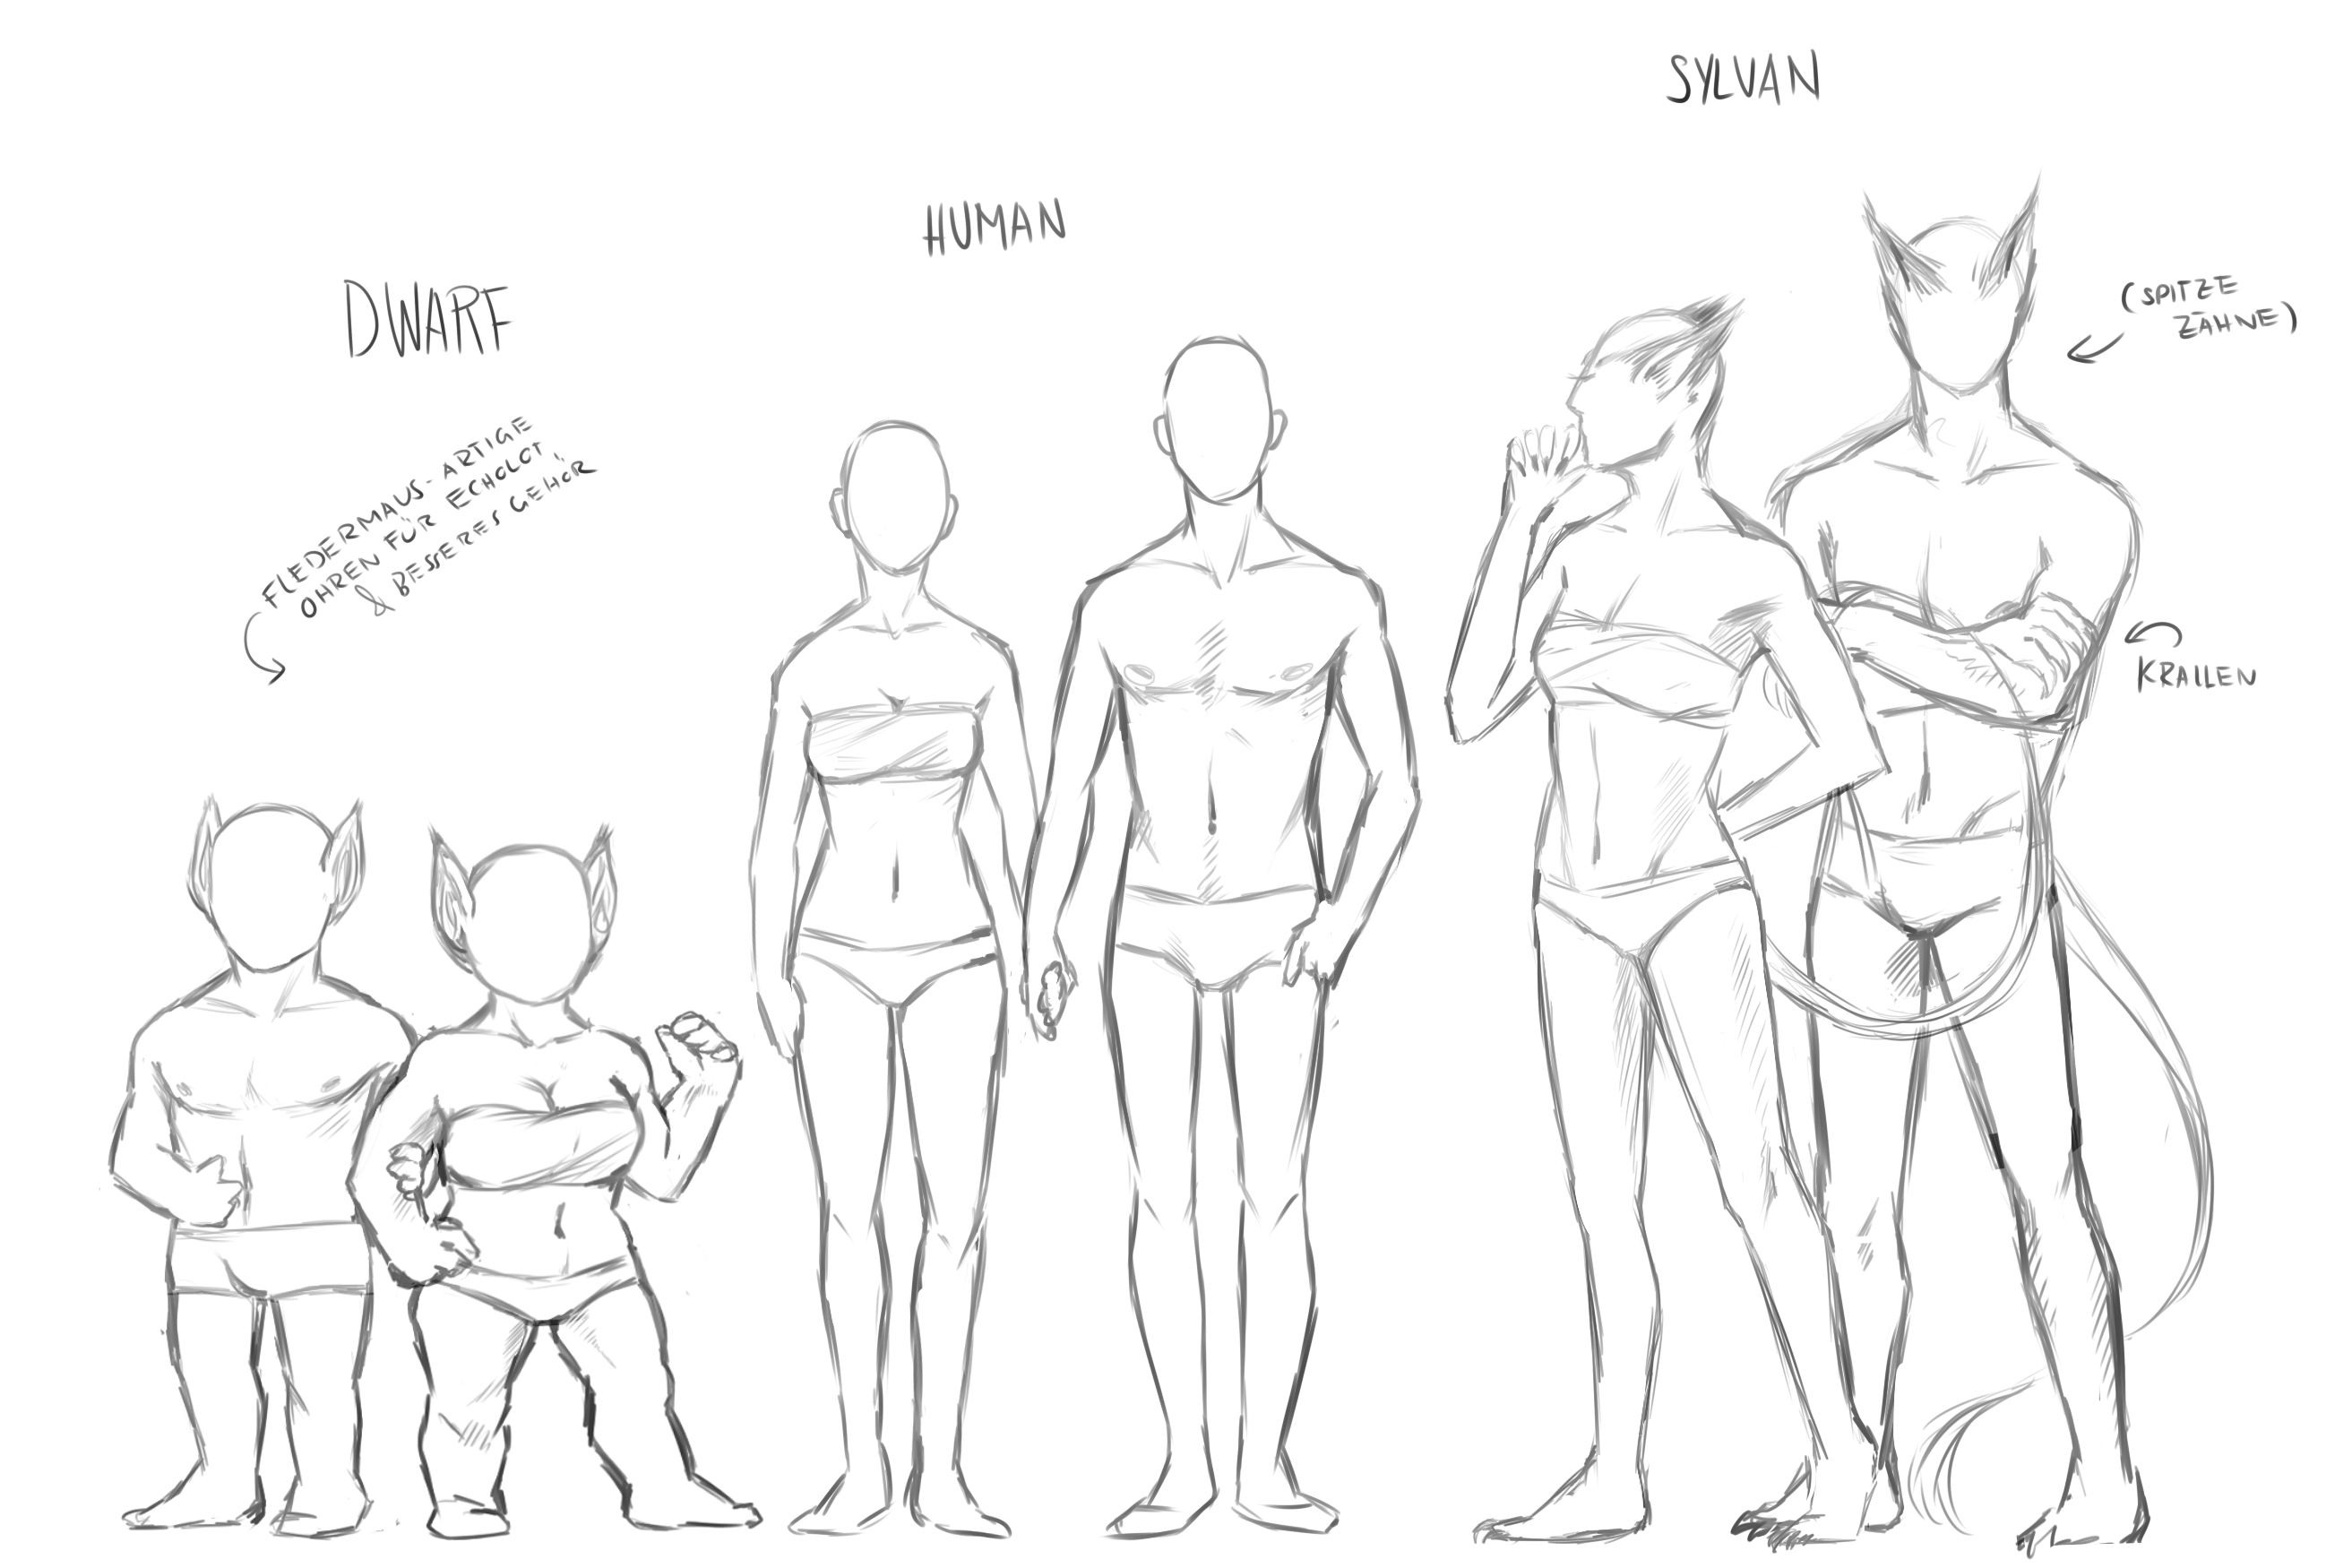
\includegraphics[width=1.0\linewidth]{Abbildungen/Weltenbau/Lebensformen/allerassen}
	\caption{Vergleich der unterschiedlichen homininen Rassen.}
	\label{fig:allerassen}
\end{figure}


\paragraph{Stammbaum} Hier soll man später den Stammbaum der Hominini finden können. Also welche Art sich wann von welcher anderen abgezweigt hat.

\paragraph{Besonderheiten}
Einige Humanoide haben gemeinsame Besonderheiten im Vgl. zu den RL-Menschen. Dies hängt immer davon ab, wann sich die jeweiligen Arten voneinander abgespalten haben. \\
So haben z.B. alle Humanoiden ein besonderes Sinnesorgan (siehe Standard bei Menschen, Besonderheiten bei der jeweiligen Art erwähnt).


\subsection{Vorwissen}
Bei der Erstellung der Rassen bitte folgende Punkte (aus \href{https://de.m.wikipedia.org/wiki/Primaten#Merkmale}{Wikipedia}) beachten:\\
Obwohl die Primaten eine relativ klar definierte Säugetierordnung sind, gibt es relativ wenig Merkmale, die bei allen Tieren dieser Ordnung und sonst bei keinem anderen Säugetier zu finden sind. Dennoch lassen sich laut dem Biologen Robert Martin neun Merkmale der Primatenordnung festhalten:
\begin{itemize}
	\item Der große Zeh ist opponierbar (Ausnahme: Mensch) und die Hände sind zum Greifen geeignet.
	\item Die Nägel an den Händen und Füßen der meisten Arten sind flach (keine Krallen). Zudem haben Primaten Fingerabdrücke.
	\item Die Fortbewegung ist von den Hinterbeinen dominiert, der Schwerpunkt liegt näher an den hinteren Gliedmaßen.
	\item Die olfaktorische Wahrnehmung ist unspezialisiert und bei tagaktiven Primaten reduziert.
	\item Die visuelle Wahrnehmung ist hochentwickelt. Die Augen sind groß und nach vorne gerichtet (Stereoskopie).
	\item Die Weibchen haben geringe Wurfgrößen. Schwangerschaft und Abstillen dauern länger als bei anderen Säugetieren vergleichbarer Größe.
	\item Die Gehirne sind verhältnismäßig größer als bei anderen Säugetieren und weisen einige einzigartige anatomische Merkmale auf.
	\item Die Backenzähne sind relativ unspezialisiert und es gibt maximal drei; sowie maximal zwei Schneidezähne, einen Eckzahn, und drei Prämolare.
	\item Es gibt weitere (für Systematiker nützliche) subtile anatomische Besonderheiten, die sich jedoch nur schwer funktionell einordnen lassen.
	\item \textbf{Körpergröße:} Einige Arten haben einen ausgeprägten Geschlechtsdimorphismus, wobei die Männchen mancher Arten doppelt so schwer wie die Weibchen sein können und sich auch in der Fellfarbe unterscheiden können. 
	\item \textbf{Behaarung:} Der Körper der meisten Primaten ist mit Fell bedeckt, dessen Färbung von weiß über grau bis zu braun und schwarz variieren kann. Die Handflächen und Fußsohlen sind meistens unbehaart, bei manchen Arten auch das Gesicht oder der ganze Kopf (zum Beispiel Uakaris). Am wenigsten behaart ist der Mensch. 
	\item \textbf{Augen:} Die größten Augen aller Primaten haben die Koboldmakis. Bei den größtenteils nachtaktiven Feuchtnasenprimaten ist zusätzlich eine lichtreflektierende Schicht hinter der Netzhaut, das Tapetum lucidum vorhanden.
	\item \textbf{Nase:} Namensgebender Unterschied der beiden Unterordnungen ist der Nasenspiegel (Rhinarium), der bei den Feuchtnasenprimaten feucht und drüsenreich ist und sich in einem gut entwickelten Geruchssinn widerspiegelt. Die Trockennasenprimaten hingegen besitzen einfache, trockene Nüstern und ihr Geruchssinn ist weit weniger gut entwickelt. 
	\item \textbf{Zähne:} Die Form insbesondere der Backenzähne gibt Aufschluss über die Ernährung. Vorwiegend fruchtfressende Arten haben abgerundete, insektenfressende Arten haben auffallend spitze Molaren. Bei Blätterfressern haben die Backenzähne scharfe Kanten, die zur Zerkleinerung der harten Blätter dienen. 
	\item \textbf{Schwanz:} Für viele baumbewohnende Säugetiere ist ein langer Schwanz ein wichtiges Gleichgewichts- und Balanceorgan, so auch bei den meisten Primaten. Jedoch kann der Schwanz rückgebildet sein oder ganz fehlen. Mit Ausnahme der Menschenartigen, die generell schwanzlos sind, ist die Schwanzlänge kein Verwandtschaftsmerkmal, da Stummelschwänze bei zahlreichen Arten unabhängig von der Entwicklung vorkommen. Sogar innerhalb einer Gattung, der Makaken, gibt es schwanzlose Arten (zum Beispiel der Berberaffe) und Arten, deren Schwanz länger als der Körper ist (zum Beispiel der Javaneraffe). Einen Greifschwanz haben nur einige Gattungen der Neuweltaffen ausgebildet (die Klammerschwanzaffen und die Brüllaffen). Dieser ist an der Unterseite unbehaart und mit sensiblen Nervenzellen ausgestattet.
	\item \textbf{Aktivitätszeiten:} Die unterschiedlichen Aktivitätszeiten haben sich auch im Körperbau niedergeschlagen, so sind in beiden Untergruppen nachtaktive Tiere durchschnittlich kleiner als tagaktive. Eine weitere Anpassung an die Nachtaktivität stellt der bessere Geruchssinn der Feuchtnasenprimaten dar. Vergleichbar mit anderen Säugetieren ist die Tatsache, dass Arten, die sich vorwiegend von Blättern ernähren, längere Ruhezeiten einlegen, um den niedrigen Nährwert ihrer Nahrung zu kompensieren. 
\end{itemize}


\subsection{Menschen} \label{rasse:mensch}
\begin{itemize}
	\item sehen an sich wie Menschen aus. Durchschnittliche Körpergröße: 165 cm für Frauen, 180 vm für Männer
	\item zusätzliches Sinnesorgan zum Spüren von Magie. Dieses funktioniert ähnlich wie das Seitenlinienorgan der Fische. Öffnungen am Hals links und rechts erlauben die Wahrnehmung von Magie bzw. deren Intensität. Man kann sie spüren wie Druck. Siehe auch Abb. \ref{fig:sinnesorganauswahl}.
\end{itemize}

\begin{figure}
	\centering
	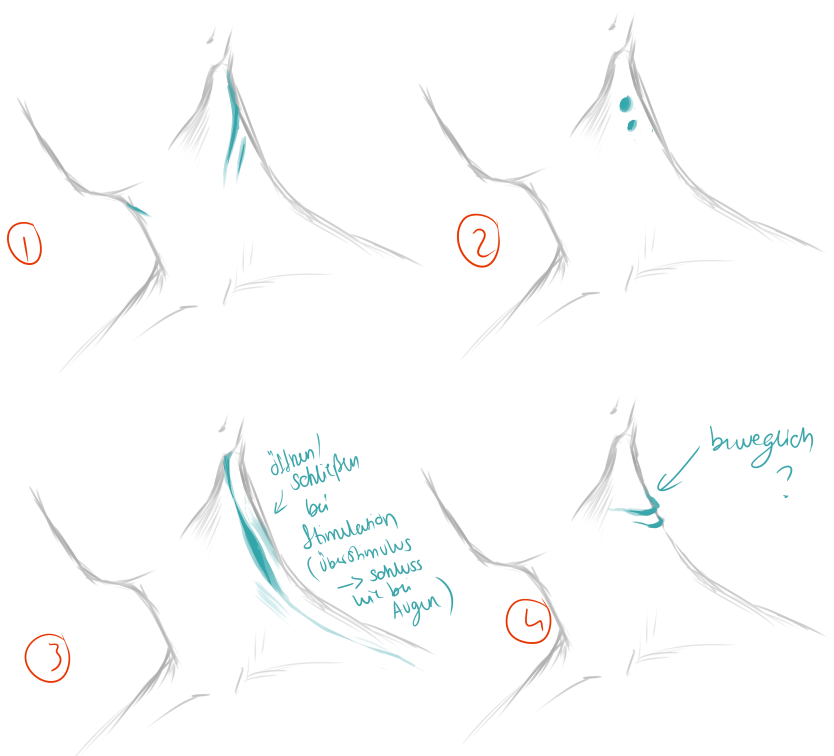
\includegraphics[width=0.7\linewidth]{Abbildungen/Weltenbau/Lebensformen/Sinnesorgan_Auswahl}
	\caption{Die möglichen Formen eines Sinnesorgans zum Spüren von Magie.}
	\label{fig:sinnesorganauswahl}
\end{figure}

\subsection{Dunkles Volk}

\subsection{Zwerge} \label{rasse:zwerge}
\begin{itemize}
	\item  Zwerge sind "kleine", stämmige Menschen (da solche durch Tunnel besser hindurch kommen) mit einer Körpergröße von durchschnittlich 1,25 m bei Frauen und 1,35 m bei Männern. Dabei sind die Gräbern sehr Kräftige aufgrund der anstrengenden körperlichen Arbeit, wie in Abb. \ref{fig:zwerggraeber} zu sehen ist. Die restlichen sind wie Menschen unterschiedlichen Körperbaus, zu sehen in Abb. \ref{fig:zwergkaufmann} und\ref{fig:zwerghaendlerin}. Ihr Körper ist bezgl Kopf und Torso vergleichbar mit Menschen, doch ihre Gliedmaßen scheinen verkürzt.
	\item leben in Höhlensystemen die tief unter die Oberfläche reichen
	\item ihre \textbf{Sicht} ist nicht so gut, da das im Allgemeinen recht unwichtig unter der Erde ist
	\item dafür ist ihr \textbf{Gehör} extrem gut. Zudem können sie (ähnlich wie Fledermäuse) auch höhere und tiefere Schwingungen wahrnehmen und sie zur Orientierung nutzen. Sie haben zwar kein Organ, um diese Schallwellen so auszustoßen, allerdings zeigt sich das in ihrer Magie. Ihre Ohren sind dadurch etwas abstehender und deutlich beweglicher (ähnlich mehrere Tiere, zB auch Fledermäuse)
	\item auch ihr \textbf{Geruch} ist verbessert: mit diesem können sie schnell gefährliche Dämpfe wahrnehmen oder Beutetiere unter der Erde riechen.
	\item Magie-bezogen hat sich bei ihnen nämlich hauptsächlich die \textbf{\npref{sec:vibrationsmagie} (änderbar)} durchgesetzt: damit können sie die Schwingungen in der Luft erzeugen, die sie mit ihrem feinen Gehör auswerten und sich so auch im Dunklen zurechtfinden können. Weiterhin nützt ihnen die Vibration beim Tunnelbau sehr viel
	\item weiterhin hat sich ihre \textbf{Sauerstoffverwertung} angepasst: sie sind in der Lage, schon geringe Mengen Sauerstoff in der Umgebungsluft effektiv zu nutzen und somit auch tief unter der Erde vernünftig atmen zu können. Diese erhöhte Verwertbarkeit ist ein gradueller Anpassungsprozess, der nicht von jetzt auf gleich funktioniert. Das ist vor allem beim Aufstieg aus den Tiefen relevant, denn wenn sie zu schnell an die Oberfläche mit ihrer hohen Sauerstoffkonzentration kommen, dann erleiden sie Symptome wie bei der Hyperventilation und sterben. Daher müssen sie die ersten Stunden bis Tage eine Art Maske/Sack mit sich herum tragen, mit der sie sich graduell an die höhere Konzentration gewöhnen können. Weiterhin beschleunigt die hohe O2-Konzentration ihre Zellalterung und somit ihren Tod. Dies führt dazu, dass sie sich auf der Oberfläche kaum finden lassen  und vorrangig mehrere Meter tief unter der Erde wohnen.
\end{itemize}

\begin{figure}
	\centering
	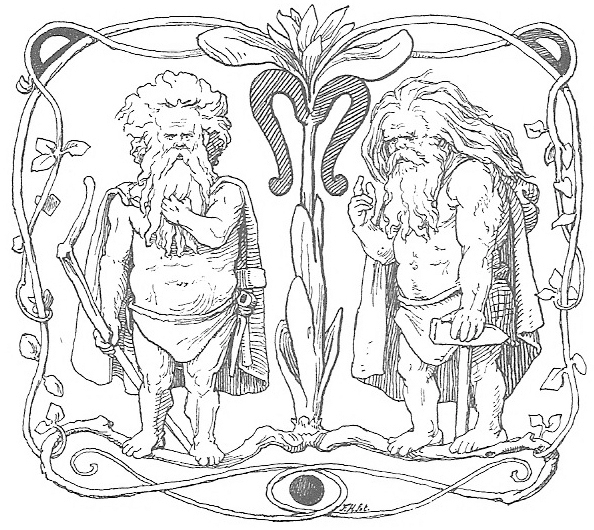
\includegraphics[width=0.7\linewidth]{Abbildungen/Weltenbau/Lebensformen/ZwergGraeber.png}
	\caption{Typische Gräber der Zwerge.}
	\label{fig:zwerggraeber}
\end{figure}

\begin{figure}
	\begin{minipage}{0.49\textwidth}
		\centering
		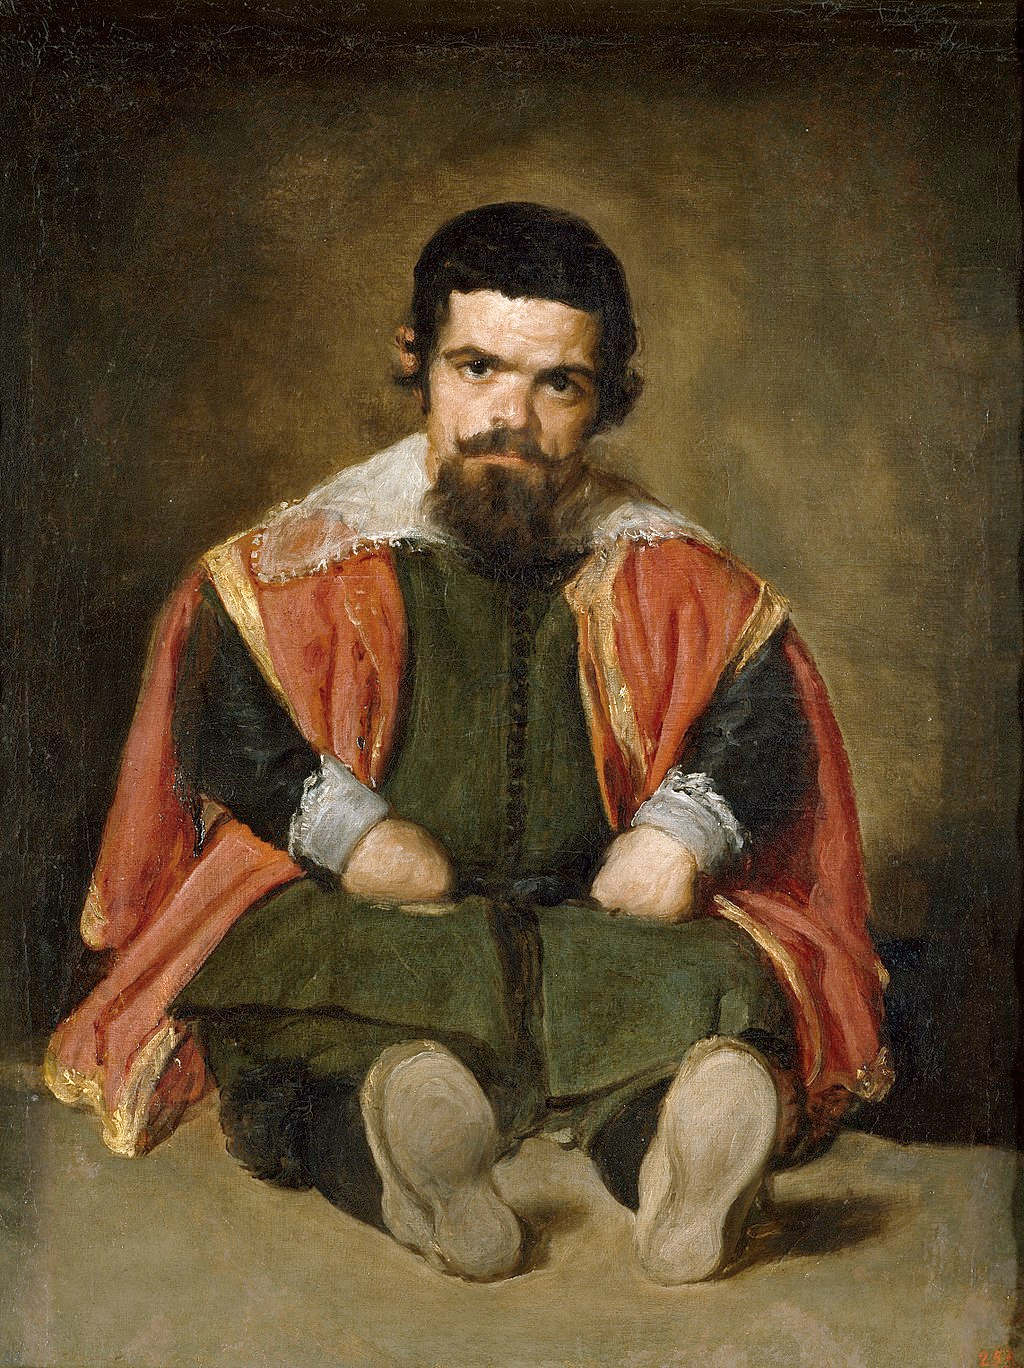
\includegraphics[width=0.8\linewidth]{Abbildungen/Weltenbau/Lebensformen/ZwergKaufmann.png}
		\caption{Ein zwergischer Kaufmann.}
		\label{fig:zwergkaufmann}
	\end{minipage}
	\hfill
	\begin{minipage}{0.49\textwidth}
		\centering
		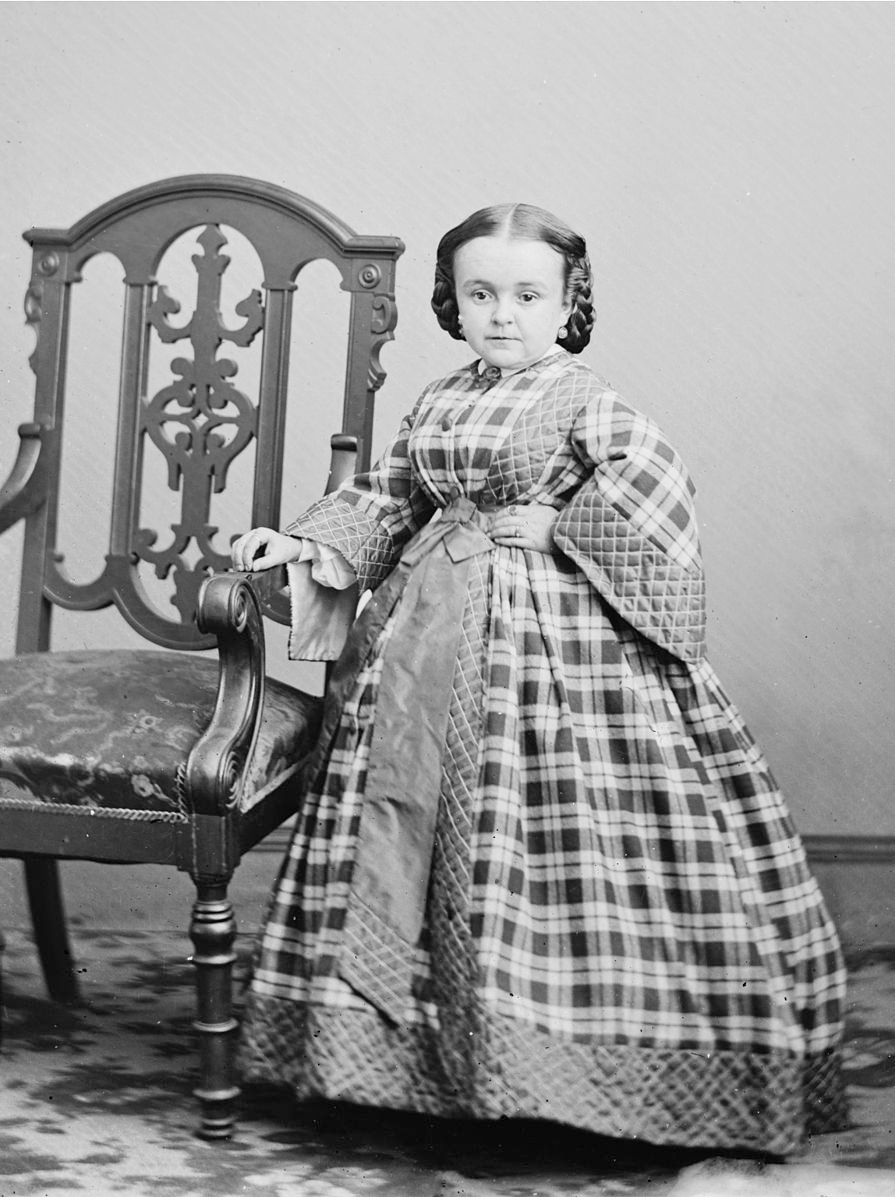
\includegraphics[width=0.8\linewidth]{Abbildungen/Weltenbau/Lebensformen/ZwergHaendlerin.png}
		\caption{Eine zwergische Händlerin.}
		\label{fig:zwerghaendlerin}
	\end{minipage}
\end{figure}



\subsubsection{Entstehung der Zwerge}
Die Vorfahren der Zwerge, eine Menschenaffenart normaler Größe, sind eine Gruppe, die sich in einer Gegend niedergelassen hatten, die einen gefährlichen größeren Jäger hatte. Das zwang diese Menschen dazu, sich in die natürlichen Höhlen der Gegend zurück zu ziehen. Die Jagd bei Nacht wurde bevorzugt, da es tagsüber gefährlicher war. Über die Zeit hinweg passten sie sich ihren Bedingungen an: Leben hauptsächlich im Dunklen und unter der Erde, draußen nur nachts. Für eine wachsende Gemeinschaft schließlich mussten immer tiefere Höhlen gegraben werden und so... kam es zur Entwicklung der Rasse der Zwerge, wie es sie heute gibt



\subsection{Halblinge} \label{rasse:halblinge}
Ziemlich genau \href{https://de.wikipedia.org/wiki/Pygm\%C3\%A4en}{Pygmäen}.


\subsection{Sylvan} \label{rasse:sylvan}
ein Sylvan, mehrere Sylvaner
\begin{itemize}
	\item diese Menschenart lebt in dem \npref{formation:gigantus}, wo die Bäume so hoch werden, dass wir im Vgl. so groß wie Mäuse oder Käfer sind
	\item Sie leben auf den Ebenen über dem Boden, wo die riesigen Äste der Bäume neue Ebenen erschaffen. Seltenst betreten sie den Waldboden
	\item Ich stelle sie mir allerdings auch nicht am Ast schwingend vor, schon als Baumbewohner wie Menschen sie werden würden, also Natur unterwerfend und nutzen.
	\item aufgrund des extremen Vorteils der Fähigkeit, Druck bzw Wind zu beeinflussen, ebenso wie die Atombindungen zu verhärten; aufgrund dessen haben diese Allele alle anderen verdrängt und man findet bei dieser Menschenart keine andere Magienutzung mehr
\end{itemize}

\subsubsection{Aussehen der Sylvaner}
\begin{itemize}
	\item sie sind etwas größer als normale Menschen (Durchschnitt 15 cm größer: Frauen 180 cm, Männer 195 cm), deutlich dünner und bewegen sich sehr grazil
	\item eine ihrer Anpassungen an den Lebensraum: der \textbf{Schwanz}. Sie haben den Schwanz wieder rückentwickelt, weil der sehr stark bei der Stabilisation des Gleichgewichts hilft, was in den luftigen Höhen des Lebensraums von starkem Vorteil ist
	\item keine \textbf{Krallen} (sie sollen nicht zu sehr zu Mensch+Katze oder Fuchs werden). Zudem: wozu brauchen sie diese? Sie behindern beim benutzen von Werkzeugen. Vllt ein paar längere Finger oder größere Hände, im Verhältnis. 
	\item \textbf{Behaarung}. Wir möchten ungerne, dass ihnen die Menschlichkeit zu sehr abhanden kommt und sie zu sehr „Monster“ werden. Also lange Haare am ganzen Körper wären komisch. Kurze Haare, so 0,5-2 cm in der Variation plus Kopfbehaarung halte ich für sinnvoll. Denn wir stellen da ja praktisch eine leichte Rückentwicklung mehrere Merkmale dar. Also auch Haupthaar. Hände und Füße sollten nackt sein. Das Gesicht großteils auch, dafür läuft ihre Haarlinie bis zu inklusive den Augenbrauen runter (kürzere Haare auf der Stirn, keine extra Augenbrauen) und seitlich stärker auf die Wangen rauf.\\
	Idee: Sie haben einen farblichen Fellwechsel zwischen Sommer und Winter
	\item ggf. sind die \textbf{Augen} größer (Diskussion)
	\item \textbf{Ohren}: keine spezielle Anpassung, also normale menschliche Ohren
\end{itemize}

\subsubsection{Entstehung der Sylvaner}
Geschichtlich sollten sich die Sylvans recht früh von den Urmenschen abgespalten haben.

\subsubsection{Kultur}
\begin{itemize}
	\item ein Ritual könnte sein, dass sie die Leichen der Toten in Ast- und Blattwiegen aufbahren und sie dann  Richtung Erdboden schicken
\end{itemize}

\subsection{Unda}
ein Unda, mehrere Undar
\begin{itemize}
	\item diese Art lebt am Rande bzw. halb in großen Gewässern
	\item \textbf{Sonar:} In Zusammenhang mit Magie und Körperlichem haben die Undar ein präzises Biosonar entwickelt: sie können mittels Magie hochfrequentige Wellen erzeugen, mit denen sie ihre Umgebung ähnlich wie Fledermäuse abtasten. Um den Schall präzise zu interpretieren, haben sie große bewegliche Ohren. Zudem können sie mit ihrer Magie lauten Schall erzeugen, was sie gut bei der Jagd zur Betäubung einsetzen. 
\end{itemize}

\subsubsection{Körperliches}
\begin{itemize}
	\item bei ihnen entwickeln sich die Schwimmhäute an den \textbf{Händen} während der Embryonalentwicklung nicht mehr zurück; zudem haben sie vergleichsweise große und längliche \textbf{Füße} entwickelt
	\item Eine \textbf{dicke Fettschicht} schützt sie vor der Kälte des Wassers: Kaltes Wasser entzieht dem Körper wesentlich mehr Wärme als Luft. Undar müssen aber, wie die meisten anderen Säugetiere, eine konstante Temperatur von 36 bis 37 Grad Celsius halten, da sonst das Herz-Kreislauf-System versagt.
	\item Da Wasser viel dichter als Luft ist, fällt die Bewegung darin entsprechend schwerer. Mit einem ganz speziellen Trick setzen sie ihn herab: An der glatten weichen Haut würden sich beim Schwimmen normalerweise Turbulenzen bilden. Diese Verwirbelungen erhöhen den Wasserwiderstand und würden sie mit ihrer großen \textbf{Körperoberfläche} stark abbremsen. Aber Undar sind in der Lage, die entstehenden Wirbel mit Drucksensoren zu ertasten und durch feine Hautrillen auszugleichen.
	\item Da sie unter Wasser nicht atmen können, haben die Undar ihren Sauerstoffhaushalt an das Leben unter Wasser angepasst. Mit einem Atemzug können sie 80 bis 90 Prozent ihrer \textbf{Atemluft} austauschen. Beim Menschen sind es gerade einmal zehn bis 15 Prozent. Damit ihnen auf längeren Tauchgängen nicht die Luft ausgeht, können sie den Sauerstoff viel besser speichern: ihr Blut ist stärker mit Hämoglobin angereichert und sie können mehr Sauerstoff in den Muskeln zwischenspeichern. Das gesamte System der Energiegewinnung ist äußerst effizient.
	\item \textbf{Sinne:} Die meisten Wale besitzen, ähnlich wie viele andere Säugetiere, auch gut ausgebildete \textbf{Augen}. Da die Sichtverhältnisse im Wasser jedoch wesentlich schlechter sind als an Land, haben sich die Undar im Laufe ihrer Entwicklung auf andere Sinne spezialisiert, besonders auf das \textbf{Hören} und \textbf{Tasten}. Das \textbf{Riechen} ist eher unterentwickelt.
\end{itemize}

\subsubsection{Entstehung der Undar}
...

\section{Tiere}
\subsection{Echte Tiere}
\paragraph{Regenbogen Oktopus} Könnte tatsächlich eine Inspiration für Meerjungfrauen gewesen sein (insbes. Start des Videos): \href{https://img-9gag-fun.9cache.com/photo/aVYpQVK\_460svvp9.webm}{9gag.com}
\paragraph{Axolotl} Sind einfach süß. Wir wollen sie dabei haben!

\section{Pflanzen}
\subsection{Echte Pflanzen}
\paragraph{Sandbüchsenbaum} \href{https://de.wikipedia.org/wiki/Sandb\%C3\%BCchsenbaum}{Wikipedia}. Die Stacheln des Baumes sind voller Gift. Die Früchte sehen wie kleine Kürbisse aus und wenn sie reif sind, explodieren sie und schleudern die Samen mit bis zu 240 km/h weg.

\section{Mikroorganismen}



\part{Geschichte}
\chapter{Welt}
\chapter{Kontinent}
\section{Nachbarland 1}
\subsection{Kurzbeschreibung}
\begin{itemize}
	\item Name: 
	\item Lage:
	\item Topographie:
	\item ansässige Rassen:
	\item Regierung:
	\item Wirtschaft:
	\item politisches Verhältnis zu unserem Land: neutral, potentiell feindlich
\end{itemize}

\subsection{Geschichte}
Das einstige Königreich (NaLa) wird derzeit von einer Katastrophe in die andere gejagt.
Zuerst kam es zu Aufständen gegen die Monarchie, woraus sich ein handfester Bürgerkrieg entwickelte.
Im Verlaufe dieses Bürgerkrieges kam es zu Enteignungen und viele junge Menschen verloren ihre Eltern.
Diese Situation wird nun schamlos ausgenutzt von einer militanten Bewegung (MilBe), die sich zum Ziel gesetzt hat, aus NaLa einen egalitären Staat zu machen.
Das bedeutet zwar grundlegend, dass alle Einwohner den gleichen Zugang zu den zentralen Ressourcen haben (Nahrungsmittel, Güter, Land usw.) und auch Keiner dauerhaft Macht über Andere ausüben kann.
Der soziale Status des Einzelnen soll vor allem von seinen Fähigkeiten und seinem Willen abhängen.
Es soll politische und soziale Gleichheit herrschen.
Aber damit einher geht auch, dass individueller Besitz und Eigentum nur einen nachrangigen Stellenwert haben. (Im Grunde also das Prinzip des Kommunismus.)\\
\\
Die MilBe rekrutiert viele der elternlosen Jugendlichen, die ohne Bindungen dastehen sowie Personen, die aufgrund der Enteignungen und des Bürgerkrieges keine Verbindungen zu anderen Gemeinschaften mehr haben.
Außerdem verfolgt die MilBe eine stark nationalistische Philosophie, möchte Minderheiten im eigenen Land unterdrücken und ausmerzen und das eigene Volk von Fehlerhaftigkeit befreien.
Zu einer der zu bekämpfenden Fehler gehören alle Magiebegabten, die sich gegen die MilBe stellen, da sie über zu viel Macht verfügen.
In den eigenen Reihen hingegen sieht die MilBe sehr gerne, mächtige und regimetreue Magier.\\
\\
Der letzte Monarch wurde vor kurzem durch einen blutigen, durch die MilBe angeführten Aufstand ins Exil (unser Land oder ein anderes?) vertrieben.
Jetzt beginnt die MilBe die politische Säuberung von NaLa und verfolgt, foltert und ermordet Anhänger, Sympathisanten und Unterstellte der Monarchie und des Monarchen.
Die Hauptstadt von NaLa ist bereits eingenommen und eine „Demokratie“ ist ausgerufen worden, mit dem Anführer der MilBe als Staatsoberhaupt.\\
\\
Nach den langen Kämpfen begrüßt ein Großteil der Bevölkerung nun die Truppen der MilBe jubelnd.
Ein großer Teil der Kämpfer bestand aus Kindersoldaten, die zu diesem Zeitpunkt nichts anderes als ein Leben als Soldat kannten.
Doch diese Stimmungslage kippt sehr schnell als das Staatsoberhaupt mit seinem Terrorregime beginnt.
Die Besonderheit daran: Im Gegensatz zu anderen Diktatoren will dieser sich nicht zu erkennen geben und verbirgt sich hinter den Reihen der MilBe und einer großen Regierungsstruktur.
Damit will er vermeiden, dass Anschläge gegen ihn ausgeführt werden.\\
\\
In dieser Zeit, in der das Terrorregime beginnt, befindet sich NaLa aktuell.\\
\\
Die Hauptstadt wurde komplett „evakuiert“ und die MilBe hat sich dort niedergelassen.
Wer im Verdacht steht, mit Magiern, Minderheiten wie den Zwergen, Monarchieverfechtern oder sogar Ausländern/anderen Rassen zu kollaborieren, wird mitsamt der ganzen Familie (Ehegatten und Kinder) ermordet.
Anfangs werden sie klassisch hingerichtet, doch das Metall ermüdet schnell und die MilBe will Ressourcen sparen.
Darum werden die Menschen (soll es diese oder eine andere Rasse sein?) brutal zu Tode geprügelt.
Kinder werden einfach mit den Köpfen gegen Bäume geschlagen oder von Klippen gestoßen.
Erwachsene werden gehängt, oder je nach belieben anderweitig waffenfrei ermordet. Zuvor jedoch werden alle maßlos gefoltert, um Informationen über weitere Gegner der Regimes zu erhalten.
Gefangenenlager werden errichtet und täglich hunderte Menschen(?) getötet.\\
\\
Alle übrigen Mitglieder der Gesellschaft, die nicht zur MilBe überlaufen, werden in Arbeitslager gezwungen und der bisherige Reichtum, die Infrastruktur und alles, was sich bisher in NaLa entwickelt hatte, soll niedergerissen und neu strukturiert und aufgebaut werden.
Ganz nach den Vorstellungen der MilBe.\\
\\
Aufgrund dieser Entwicklungen ist NaLa gerade vollauf mit seinen eigenen Problemen beschäftigt und wird sich aktuell weder mit unserem Land verbünden noch sich anfeinden – zumindest vorerst!
Allerdings werden mittellose Flüchtlinge in unser Land kommen, die von dort berichten und Schreckliches erlitten haben.

\subsection{Gräueltaten}
Die MilBe-Soldaten, meist jung und vom Land, trieben die Menschen(?) ohne Gnade aus der Hauptstadt.
So auch Kranke, die teilweise noch verbunden waren und deren Binden von Blut durchtränkt, teils von Angehörigen auf ihren Bahren stadtauswärts getragen, andere wiederum versuchten auf allen Vieren zu krabbeln, weil sie keine Verwandten mehr hatten und nicht mehr gehen konnten.\\
\\
Neben den Massenmorden ist eine weitere Methode der MilBe der Tod durch Arbeit.
In den Arbeitslagern müssen die Gefangenen bis zur letzten Kraft arbeiten, wer nicht mehr kann, wird aussortiert oder zum Sterben zurückgelassen.
Viele sterben in den Lagern an Unterernährung, Seuchen, Überarbeitung und Folter.\\
\\
Wer in den Lagern ankam, wurde so lange gefoltert, bis er mindestens 50 bis 60 Personen denunziert hatte.
Diese wurden dann wiederum gefangen genommen usw.\\
\\
Zwangsehen um Verwandtschaftsverhältnisse zu schwächen und den Gehorsam gegenüber der MilBe zu stärken.
Bei der Zeremonie müssen die Eheleute sagen: „Ich danke MilBe, dass sie mir gute Eltern sind und mir erlauben, einen Partner zu haben und sich um mich kümmern, als wäre ich ihr biologisches Kind.“\\
Wenn eine Frau Angst hat oder schlichtweg keinen Sex mit ihrem neuen Ehemann haben will, darf sie gefoltert oder eingesperrt werden.
Der Mann kann sich beschweren, dass er um den Vollzug der Ehe betrogen wurde oder aber der Vorfall wird der MilBe von einem Spitzel gemeldet.
Die Folgen des Verstoßes sind nicht absehbar, weshalb es in den Augen vieler Frauen besser ist, den erzwungenen Geschlechtsverkehr, der vom Staat verlangt wird, einfach geschehen zu lassen.\\
\\
Babys von Verrätern werden nicht behalten.
Sie könnten später Rache nehmen.
Darum werden sie von Untergebenen der MilBe an den Füßen gepackt und gegen Bäume geschleudert.

\section{Nachbarland 2}
\subsection{Kurzbeschreibung}
\begin{itemize}
	\item Name: 
	\item Lage:
	\item Topographie:
	\item ansässige Rassen:
	\item Regierung:
	\item Wirtschaft:
	\item politisches Verhältnis zu unserem Land: freundlich
\end{itemize}

\subsection{Geschichte}

\section{Nachbarland 3}
\subsection{Kurzbeschreibung}
\begin{itemize}
	\item Name: 
	\item Lage:
	\item Topographie:
	\item ansässige Rassen:
	\item Regierung:
	\item Wirtschaft:
	\item politisches Verhältnis zu unserem Land: freundlich
\end{itemize}

\subsection{Geschichte}

\chapter{Land}
\section{Stammesverbände}
\section{Der Untergang es dunklen Volks}
\section{Monarchie}
\section{Aufstieg der Religion}
\section{Herrschaft des Ordens}
\section{Aktuell}
\section{Nahe Zukunft}
\section{Ferne Zukunft}

\chapter{Tal}

\part{Gesellschaft}
\href{http://www.weltenbau-wissen.de/2016/02/5-rezepte-fantasy-kulturen-zivilisationen/}{Fantasy-Zivilisationen}

\chapter{Religion}
\section{Übersicht}
\begin{itemize}
	\item Der Glaube an 5 gute und 2 böse Götter.
	\item Das Symbol der Religion ergibt sich wie in Abschnitt \ref{sec:goettersymbol} erklärt aus dem Zusammenspiel der 7 Götter und ist in Bild \ref{fig:goettersymbol} dargestellt.
\end{itemize}

\begin{figure}
	\centering
	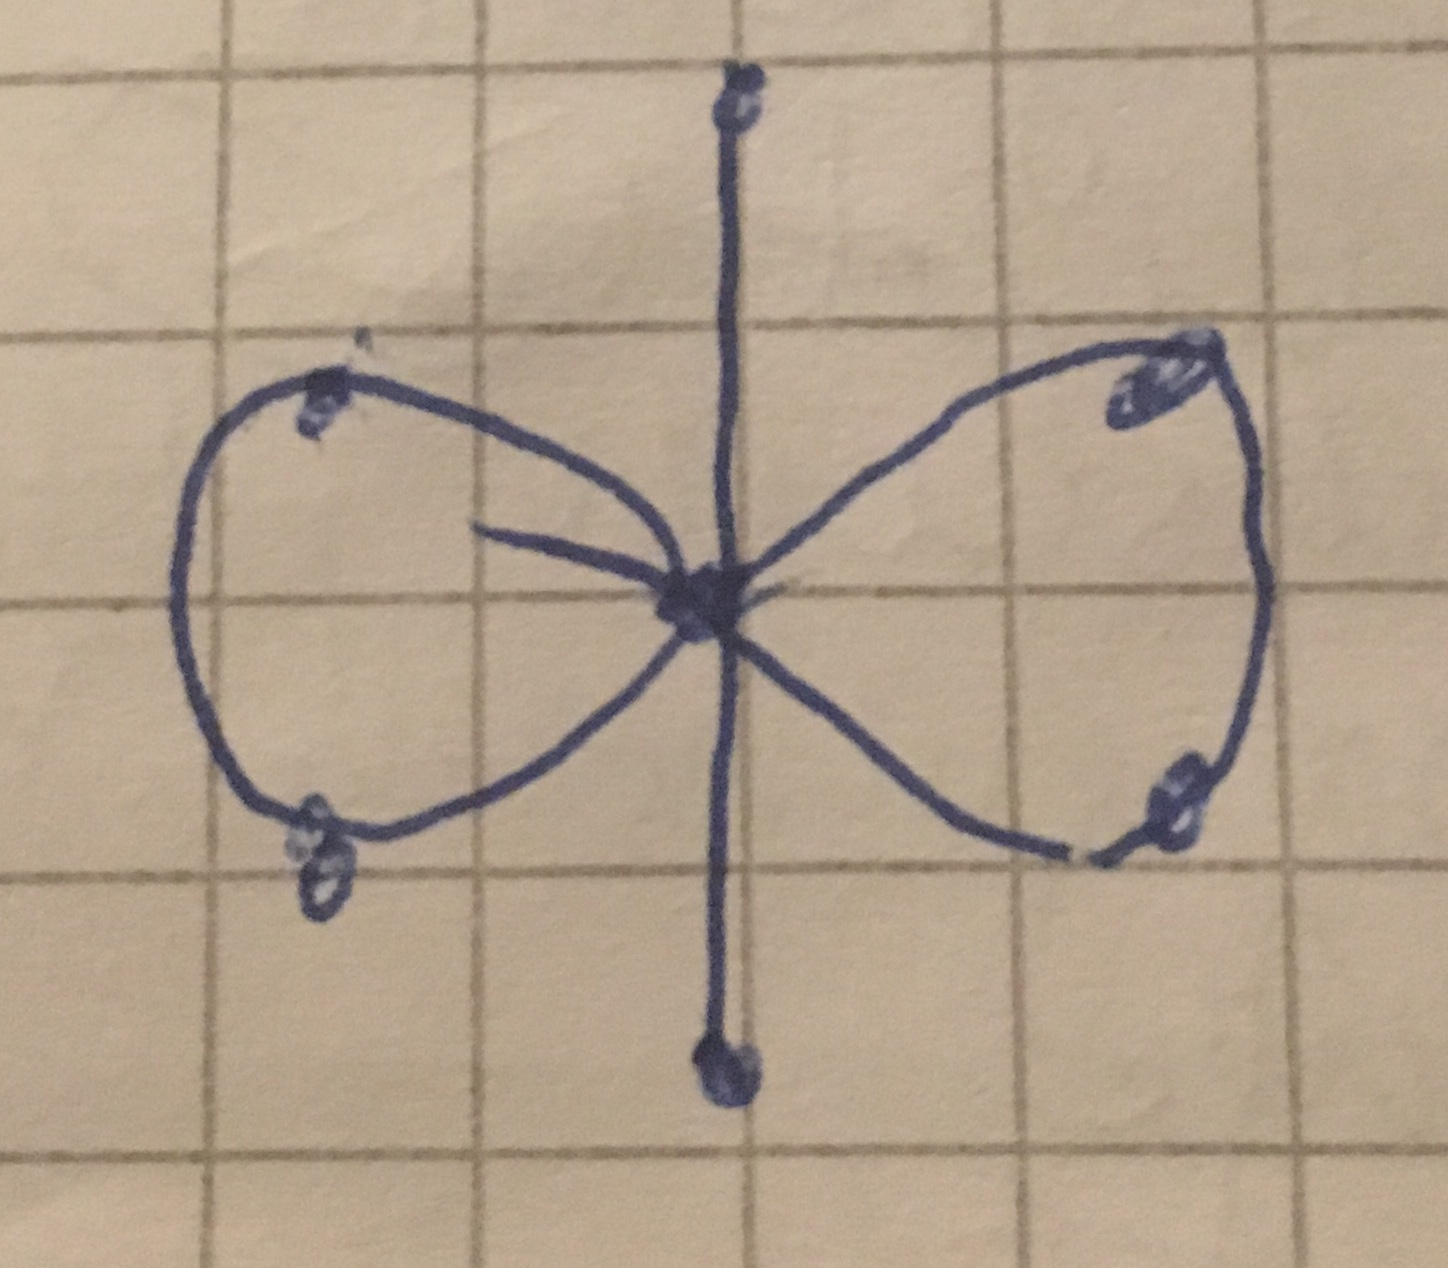
\includegraphics[width=0.3\textheight]{Abbildungen/Gesellschaft/Goettersymbol}
	\caption[Göttersymbol]{Das Symbol für die Götter}
	\label{fig:goettersymbol}
\end{figure}

\section{Geschichte}
Die hier erzählte Geschichte ist die vom Klerus verbreitete Sage über die Entstehung der Götter des Streits und der Heimtücke. \\\\
Es ist unklar, wie die Götter entstanden sind. Es geschah irgendwie irgendwann. Auf der noch recht unbewohnbaren Erde formten sie lebensfreundliches Gebiet mit ihrer jeweiligen Magie. Sie erschufen das Leben und ließen ihm seinen eigenen Lauf.\\
Nachdem sie jedoch viel Zeit damit verbracht hatten, sich an ihrem Paradies zu ergötzen, wollten sie auch Wesen nach ihrem Abbild schaffen und so lenkten sie das Leben und die Natur und brachten dadurch die Menschen hervor. Die Menschen, intelligent genug um Kultur aufzubringen, verfielen jedoch in viele Kriege. Mitgerissen aufgrund ihrer Ähnlichkeit und weil sie die Menschen so interessant fanden, integrierten sich die Götter in diese Streitigkeiten. Dabei nahmen sie die Positionen ihrer Menschengruppen an und halfen ihnen und wurden so langsam auch in einen Streit untereinander gezogen, wobei sie ihre negativen Seiten ausspielten.\\
Dies äußerte sich in vielen kleinen Dingen \textbf{(hier Geschichtchen einfügen)}, bis die Götter schließlich merkten, dass es so nicht weiter gehen kann. Sie setzten sich zusammen und kamen zum Schluss, dass sie, um wahre Leiter und Lenker des Lebens zu sein, ihre negativen Aspekte los werden müssten. Andernfalls würden ihre dunklen Seiten sie immer wieder übermannen können, was bereits große negative Folgen für alle Lebewesen hatte und auch wieder haben könnte.\\
Darum bereiteten die Götter ein Ritual vor, um perfekt zu werden und sich wortwörtlich von ihren schwachen Seiten rein zu waschen. Dazu begaben sie sich in einen See weitab der Zivilisation. Sie wuschen ihre schlechten Seiten von sich ab und versiegelten diese im See. \textbf{Allerdings gibt es ein kleines Leck, durch welches kontinuierlich ein wenig von der Magie und dem Schlechten austritt.}\\
Danach treten die Götter lange Zeit nicht in Erscheinung. In der Nähe des Sees, den Bach hinunter, lebte ein Paar. All sein Trinkwasser nahm es aus dem Bach und all ihre Ernte wurde mit dem Wasser bewässert. So nahmen sie über Zeit immer mehr von dem Bösen in sich auf. So wie ihre Macht und Magie wuchs, tat es auch das Böse in ihnen und verzehrte ihre guten Geister. Sie begannen aktiv das Böse aus der Umwelt und schließlich dem See zu absorbieren und wurden immer mächtiger und verdorbener. Sie führten Verwüstung und Zwist herbei und die Götter wurden auf sie aufmerksam. Ihre Versuche, sie zu bekämpfen und unter Kontrolle zu bekommen, scheiterten unter großen Verlusten in der Umwelt. Schließlich sahen die Götter ein, dass sie die beiden nicht besiegen konnten und unter all ihrer gebündelten Macht, um alle Lebewesen zu schütze, ersannen sie einen radikalen Plan.\\
Da die Götter zu verantworten hatten, dass diese Monster auf die Welt kamen, sahen sie es als ihre Pflicht, die Welt auch wieder von ihnen zu befreien. Aufgrund der zuvor genannten Umstände war die Maßnahme jedoch von drastischer Natur: sie hoben den Ort, auf dem sie die beiden bekämpften, aus der Erde heraus in den Himmel. Dort werden sie nun für alle Zeit gegen die beiden kämpfen und sie in Schach halten, damit das Leben auf der Erde geschützt ist.\\
Doch die beiden Bösen versuchen ihre Macht zu vergrößern, indem sie ihre Aktuelle auch dazu nutzen, den Lebewesen auf der Erde Böses einzuflüstern und sie zu manipulieren. \textbf{Die Erdenwesen sollen ihnen dienen.}\\
Bevor die guten Götter die Erdmasse mitsamt den Bösen in den Himmel aufgehoben haben, \textbf{erschufen sie gemeinsam einen Führer für die Toten}, der die verstorbenen Seelen zu ihnen bringen soll. Im Laufe der Zeit, in der sie ihre Pflichten als Götter und Führer der Welt etwas außen vor ließen, haben sie es geschafft, die Bösen zurück zu treiben. Nun gibt es nur noch Kampf auf einem kleinen Teil des Himmels-Brockens.\\
Nachdem die Toten verbrannt wurden, steigen ihre Seelen in den Himmel auf. Wenn die Verstorbenen in ihrem Leben gut waren und sich nicht von den Einflüsterungen der bösen Götter haben verführen lassen, werden sie vom Seelenleiter hinüber geführt, auf dass sie mit ihrer Kraft die Götter unterstützen und in ihrem Paradies wohnen können. Die verdorbenen Seelen jedoch werden vom Seelenleiter in die Irre geführt, damit sie nicht den Bösen helfen können, und verlieren sich in der unendlichen Dunkelheit.

\section{Götter}
In dem Land, in dem wir uns befinden, gibt es mehrere Götter. Regional unterscheidet sich die Wahl der bevorzugten Götter.
Diese sind Fiktion und existieren nicht wirklich; es gibt also auch keine Wunder, die von ihnen gewirkt werden. Allerdings interpretieren Menschen ja gerne sehr viel und sehen deshalb ein paar Dinge als Wunder an, die z.B. von den Priestern gemacht werden. Weil diese Priester gute Magier sind, aber das alles natürlich als Geschenk der Götter sehen.\\

Die Ausführungen im Folgenden stellen den Pantheon dar, wie er zur Zeit des Spiels angebetet wird. Alle Namen sind vorläufig und mehr Möglichkeit gesehen, den Göttern und 
benannten Orten etwas mehr Griffigkeit zu geben. Die Details, die im Folgenden gegeben werden (insbesondere die beispielhafte Mythen und Erzählungen über die Götter) dienen 
der Anschaulichkeit für uns und müssen sich nicht zwingend im Spiel wiederfinden.

\subsection{\textbf{Asdar} - Gott der Führung und des Schutzes}
Asdar ist der Anführer der Götter - nicht aufgrund außergewöhnlicher Stärke oder Charisma - Asdar ist nicht mächtiger als seine Mitgötter, sondern weil es seinem Wesen entspricht. Asdar ist standhaft, mutig und 
vertritt Führung durch Vorbild. Da, wo die Schutzbedürftigen verteidigt oder Verlorenen angeleitet werden müssen, ist Asdar in der ersten Reihe zu finden. \\
\begin{itemize}
	\item Aussehen 
	\begin{itemize}
		\item großer Mann im mittleren Alter
		\item kurze silberne Haare
		\item häufig in Rüstung und mit alten Kampfnarben
	\end{itemize}
	\item Aspekte
	\begin{itemize}
		\item Herrschaft und Führung
		\item Kampf und Schutz
		\item Vertreibung von Übel
	\end{itemize}
	\item Tugenden Asdars
	\begin{itemize}
		\item Standhaftigkeit, Mut
		\item körperliche Stärke und Macht
		\item Opferbereitschaft
	\end{itemize}
\end{itemize}
\textit{Weit bekannter Mythos Asdars}:\\
Vor Urzeiten, als die Welt noch jünger war, streiften mächtige Monster durch die Lande und verbreiteten Angst und Schrecken. Es begab sich, dass Asdar, als einfacher Wanderer 
verkleidet, in einem Dorf Herberge suchte. Ein Lindwurm, eine mächtige Bestie mit einer geschuppten Haut härter als Stein und Klauen und Zähnen größer und schärfer als das 
beste Schwert der Menschen, fiel über das Dorf her, getrieben von unstillbarer Gier und Hunger. Und Asdar offenbarte sich in seiner Rüstung und sprach: ``Wer bereit ist, sein Heim 
und seine Familie zu verteidigen, der nehme seine Waffe und kämpfe an meiner Seite.'' Und die Menschen folgten seinem Ruf, gewappnet mit jedweder Waffe die sie finden konnten. 
Der Kampf war lang und schwierig und manch einer wäre dem Hunger des Wurms zum Opfer gefallen, wenn Asdar die Angriffe nicht mit Schild und Rüstung abgefangen hätte. Doch 
mit seinem letzten Atemhauch gelang es dem Lindwurm noch, Klaue an Asdar zu legen und ihm eine weitere Narbe zu verpassen.\\~\\

positive Gemüter: Mut, Macht, Kraft, Würde, Standhaftigkeit, Entscheidungsvermögen, Führungsqualitäten, Sicherheit, Intuition, Schutz



\subsection{\textbf{Bouda} - Göttin der Harmonie und des Wachstums}
Bouda ist die schaffende Gottheit des Pantheons. Nach ihrem Willen erwachsen neue Pflanzen in jedem Frühling, um den Hunger aller zu stillen. Nach ihrem Wilen wird das Band 
der Ehe geformt, das Mann und Frau in Harmonie miteinander verbindet. Bouda akzeptiert alle als ihre Kinder und schenkt die Fähigkeit, zu vergeben und zu versöhnen.\\
\begin{itemize}
	\item Aussehen 
	\begin{itemize}
		\item ``Mutterfigur''
		\item mittleres Alter 
		\item kräftige Figur
		\item alltägliche Kleidung 
	\end{itemize}
	\item Aspekte
	\begin{itemize}
		\item Familie (Ehe und Elternschaft)
		\item Ernte und Wachstum
		\item Heilung
	\end{itemize}
	\item Tugenden Boudas
	\begin{itemize}
		\item Gnade und Demut
		\item Offenheit und Akzeptanz
		\item nichterotische Liebe
	\end{itemize}
\end{itemize}
\textit{Weit bekannter Mythos Boudas}:\\
Vor Urzeiten, als die Welt noch jünger war, lagen die Reiche der Menschen beständig im Streit miteinander. Päkte wurden geschmiedet und gebrochen, ein Herrscher folgte auf den 
nächsten und keiner vermochte es, andauernden Frieden zu finden. Doch manchmal schmiedete das Schicksal seltsame Bande: es begab sich nämlich, dass die Thronfolger zweier 
verfeindeter Reiche in demselben Wald jagten und von einem Sturm von ihren jeweiligen Wegen abgebracht und in der 
Hütte einer alten Frau zusammengebracht wurden. Und als die beiden sich der Anziehung bewusst wurden, die zwischen ihnen zu erblühen begann, baten sie die alte Frau, ihre
Vermählung vor Bouda zu bezeugen, auf dass selbst ihre Väter sie nicht mehr trennen könnten. Und die alte Frau schenkte ihnen zur Mitgift zwei Armreife, die das Band ihrer Vereinigung 
darstellen sollten. Und als die beiden Thronfolger heimkehrten, kam Friedfertigkeit über jeden, der die Reife der beiden sah. Und zum ersten Mal seit langem herrschte Frieden 
zwischen den Nationen.\\~\\

positive Gemüter: Familie, Liebe, Selbstlosigkeit, Gnade, Mitgefühl, Vergebung, Demut, Reinheit, Frieden, Toleranz, Geborgenheit, Harmonie

\subsection{\textbf{Erlin} - Gott des Ausgleichs und der Gerechtigkeit}
Erlin lehrt die Menschen, die Bindungen zu ihren Mitmenschen ausgewogen zu halten. Sowohl Respektlosigkeit als auch übermäßige Ehrerbietung versäuern das Verhältnis 
zu den Mitmenschen und müssen daher vermieden werden. Dazu gehört, sich an die Gesetze und Regeln der Gesellschaft zu halten.\\
\begin{itemize}
	\item Aussehen 
	\begin{itemize}
		\item alter Mann 
		\item hochgewachsen und hager
		\item in makelloser Robe, aufrechte Haltung
		\item Richthammer am Gürtel
	\end{itemize}
	\item Aspekte
	\begin{itemize}
		\item Gesetzgebung und Rechtsprechung
		\item Handel
		\item Weises Vorgehen \footnote{Leichte Überschneidung mit Faelans Aspekt}
	\end{itemize}
	\item Tugenden Erlins
	\begin{itemize}
		\item Disziplin und Respekt
		\item stoisch und gelassen
		\item streng mit sich selbst und Anderen
	\end{itemize}
\end{itemize}
\textit{Weit bekannter Mythos Erlins}:\\
<Erlin fällt eine Richtspruch über ...>\\~\\
positive Gemüter: Höflichkeit, Disziplin, Gleichgewicht, Ruhe, Gelassenheit, Geduld, Wachstum, Ausgeglichenheit, Strenge, Heilung, Ausgleich, Urteilvermögen

\subsection{\textbf{Aina} - Göttin der Lebensfreude und Liebe}
Aina mag für manche wie die schwächste der Götter aussehen - ihre Mythen berichten fast ausschließlich von Festen und Kunstwerken. Und dennoch ist Aina eine der beliebtesten 
Götter im einfachen Volk. Jeder Reigen zum Mittsommerfest, jedes alkoholschwangere Fest und jeder stille (und jeder weniger stille) Moment der Zweisamkeit genießt Ainas Segen 
und Unterstützung.\\
Doch neben diesen ausgelassenen Momenten schenkt Aina auch denen Lebensfreude und Hoffnung, die diese am dringensten benötigen. Diejenigen, die von Trauer oder 
Hoffnungslosigkeit niedergedrückt werden, hilft der Glaube an das Lebenswerte, um sich wieder aufzuraffen.
\begin{itemize}
	\item Aussehen 
	\begin{itemize}
		\item junge Frau in Festtagskleidung
		\item häufig zum Lachen aufgelegt
		\item attraktiv 
	\end{itemize}
	\item Aspekte
	\begin{itemize}
		\item erotische Liebe (als Vereinigung)
		\item Feierlichkeiten
		\item Kunst und Kultur
		\item Trost und Hoffnung
	\end{itemize}
	\item Tugenden Ainas
	\begin{itemize}
		\item Kreativität und Freigeistigkeit
		\item zu Scherzen aufgelegt
		\item charmant und fröhlich
	\end{itemize}
\end{itemize}
\textit{Weit bekannter Mythos Ainas}:\\
Vor Urzeiten, als die Welt noch jünger war, waren die Menschen eitel aufgrund ihrer eigenen Fertigkeiten. Glemric, Barde und Meister seiner Zunft, war einer dieser Menschen. 
Er rühmte sich seiner Künste mit Flöte und Harfe und behauptete, dass selbst Aina selbst nicht mit ihm mithalten könne. Und so kam es, dass eines Abends, als die Nächte 
kurz und der Mittsommer nahe war, eine junge Frau vor seiner Tür stand und ihn zu einem Wettbewerb herausforderte. Gäste wurden geladen, um die Kunstfertigkeit der Kontrahenten 
zu bewerten und sich ihrer Kunst zu erfreuen. Doch jedes Stück, das Glemric aufspielte, vermochte sein Gast zu überbieten, bis letzlich sogar Glemric selbst einsehen musste, 
dass er geschlagen war. Noch an diesem Abend gelobte er, seine Ehre wiederherzustellen und sich bei seinem Gast zu revanchieren. Und so geschah es, dass Glemric ein Jahr später 
in derselben Nacht Aina zu einer Revanche herausforderte. \\~\\
positive Gemüter: Glück, Hingabe, Enthusiasmus, Fröhlichkeit, Freiheit, Menschlichkeit, Kunst, Kultur, Charme, Kreativität, Freude

\subsection{\textbf{Faelan} - Gott der Weisheit}
Weisheit kann viele Dinge bedeuten. Die Fähigkeit, Zusammenhänge zu begreifen und auszunutzen. Die Fähigkeit, den für sich selbst und Andere besten Weg zu erkennen. Und die 
Fähigkeit, aus dem Wenigen, was man hat, das Beste zu machen. Faelan verkörpert alle diese Aspekte. Einerseits ist der Gott von Wissen und 
Gelehrsamkeit, der die Menschen Schrift, Wissen und Magie lehrt. Andererseits ist - beziehungsweise war - Faelan ein Gott der Schläue und 
der günstigen Gelegenheiten, der den Menschen überlegtes und zielstrebiges Handeln beibringt. Diese zweite Seite von Faelans Wesen ist mit 
dem Erstarken des Klerus immer mehrin Vergessenheit geraten, da die Verehrung eines Gottes der Diebe und Reisenden wenig erwünscht war.\\
\begin{itemize}
	\item Aussehen 
	\begin{itemize}
		\item Junger Mann 
		\item schlank und gelenkig
		\item beständig neugierig
		\item Wissen: trägt ein Buch und einen Kohlestift mit sich
		\item Schläue: trägt einen Schlüssel und eine Kappe mit sich
	\end{itemize}
	\item Aspekte
	\begin{itemize}
		\item Weisheit und Verständnis
		\item Schrift
		\item Philosophie und andere Wissenschaften
		\item Magie
	\end{itemize}
	\item Tugenden Faelans
	\begin{itemize}
		\item Neugierig und wissbegierig
		\item Lehrend
		\item weise und beobachtend
	\end{itemize}
\end{itemize}
\textit{Weit bekannter Mythos Faelans}:\\
<Faelan stiehlt/vergibt einen Namen>  \\~\\
positive Gemüter: Erleuchtung, Wissen, Verständnis, Konzentration, Wahrheit, Klarheit, (Um-)wandlung, Zielstrebigkeit, Weisheit, Aufstieg


\subsection{\textbf{Der Flüsternde Schatten} - Gott der Heimtücke}
Der Flüsternde Schatten -auch als ``Flüsterer'' bekannt - ist ein Gott, der aus einem Mangel an Emotionen entstanden ist. Er ist manipulierend, rational und kühl. Mit einem 
wohlgesetzten Wispern schleicht er sich in die Köpfe der Menschen und lässt auch sie die Welt mit seinen Augen sehen. Und wer sich seines Flüsterns lange öffnet, der verliert 
Schritt für Schritt ebenso alle Fähigkeit zu eigenen Emotionen, bis der Mensch nicht viel mehr ist als ein lebender Schatten.\\
Aspekte: feige, gefühllos, heimtückisch, rückgratlos, eitel\\
Plage: Depression und Trauer, grausames Kalkül, selbstsüchtige Hinterlist, Fanatismus\\~\\

negative Gemüter: eingebildet, versteift, zwingend, ängstlich, heimtückisch, fanatisch, manipulativ, selbstüberschätzend, rücksichtslos, stolz, unterdrückend, hochnäsig,
überheblich, arrogant, egoistisch, rückgratslos, feige, scheu, abhängig, Faul, gefühllos, eitel, misstrauisch, zynisch, nervös, voreilig, schadenfreudig

\subsection{\textbf{Drayl} - Göttin des Streits}
Drayl ist ein Gott, der aus einem Übermaß an Emotionen erwachsen ist. Jedes Übermaß an Emotionen führt Menschen zu Konflikten, bei denen nicht die gute Sache im Vordergrund 
steht, sondern die Menschen von Drayls Willen bessessen sind. Drayl kann in vielerlei Formen erscheinen - sei es eine Axt, die einem Krieger ultimative Macht im Blutrausch 
verspricht, ein Schatz, der einen Händler zu gierigem Tun verleitet oder ein schönes Wesen, das zu hemmungsloser und aggressiver Wolllust verführt.\\
Aspekte: Wut, Neid, Gier, Chaos\\
Plage: Mania, Jähzorn, Instabilität\\~\\

negative Gemüter: gierig,  habsüchtig,  streitsüchtig, störrisch, grausam, aggressiv, undiszipliniert, neidisch, unberechenbar, unaufmerksam, jähzornig, wollüstig, völlernd, 
chaotisch, instabil, manisch

\subsection{Das Göttersymbol} \label{sec:goettersymbol}
Beim Wasser-/Reinigungsritual, dem Abtrennungsritual oder einem anderen war die Aufstellung der fünf Götter und ihr Energiefluss wie dargestellt in Abb. \ref{fig:goetteraufstellung}. Denn die stärksten und direktesten Verbindundungen/Folgen ihrer Aspekte sind so. Das ergibt eine liegende acht, also das Symbol für Unendlichkeit --> 8 als heilige Zahl; Götter und ihre Macht sind unendlich.\\
\\
Mit den zwei Bösen Göttern: diese versuchen, alles zu spalten und zu zerstören. Das wird deutlich durch die Linie, welche die 8 versucht zu zerschneiden. Zudem zeigt es aber auch, wie durch die bösen Götter und zum Schutz des Lebens, ein Stück von der Erde abgetrennt werden musste. Des Weiteren mahnt es, wie unsere Schlechten Seiten immer Versuchung und Untergang sind — aber sie sind auch ein Teil von uns und wir müssen lernen, damit umzugehen und ihnen zu widerstehen. Aus diesen Aspekten ergibt sich das endgültige Göttersymbol wie dargestellt in Abb. \ref{fig:goettersymbol}.\\

\begin{figure}
	\centering
	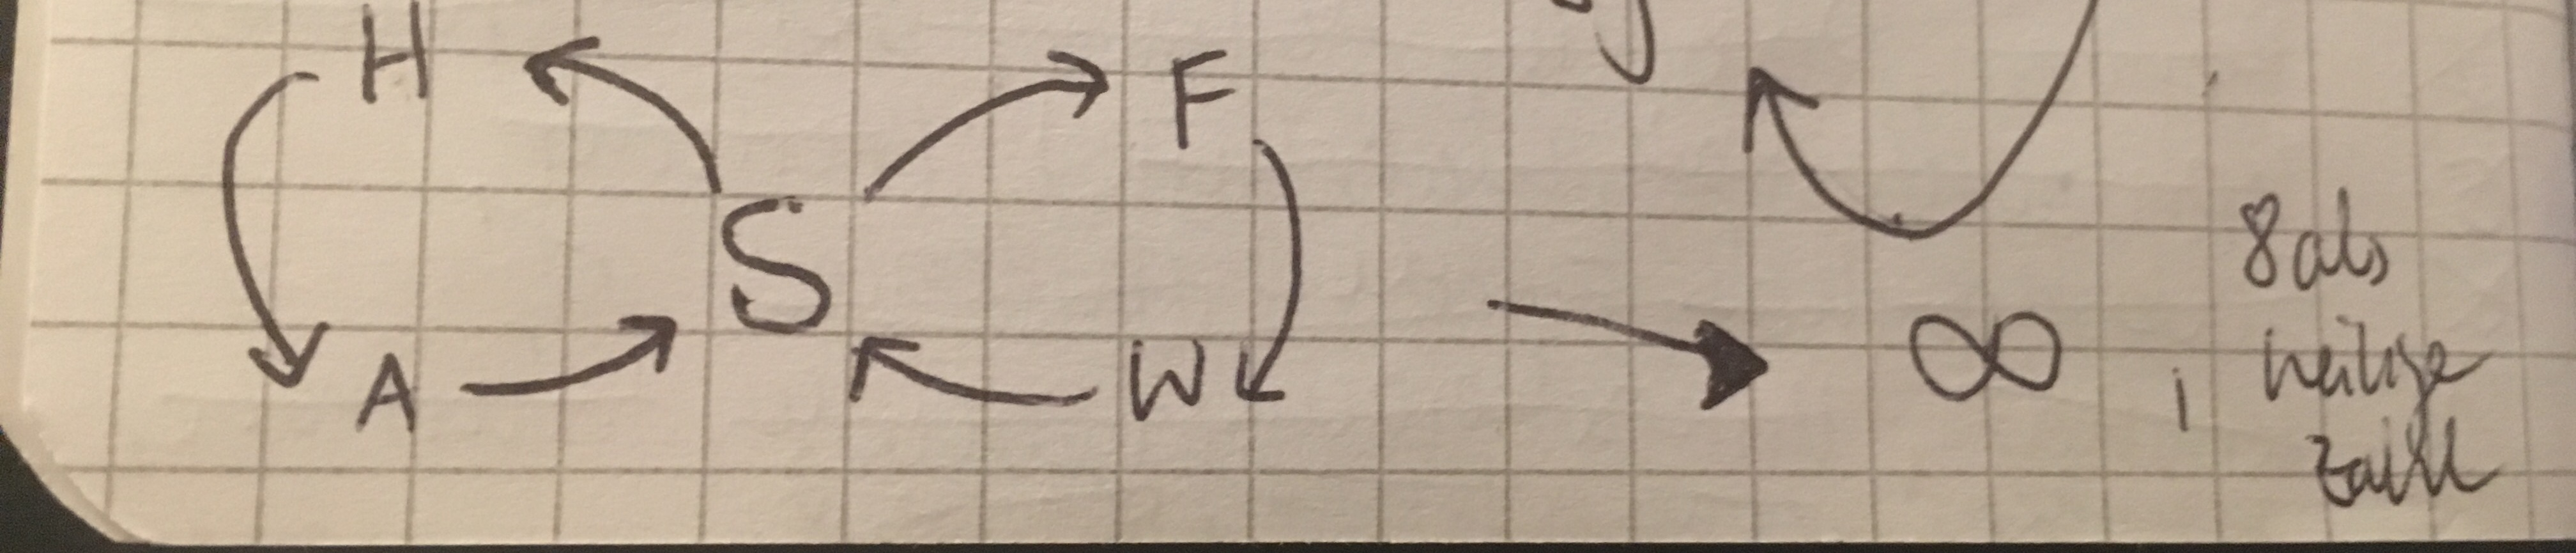
\includegraphics[width=0.7\linewidth]{Abbildungen/Gesellschaft/GoetteraufstellungbeiReinigungsritual}
	\caption{Aufstellung der Götter während des Reinigungsrituals}
	\label{fig:goetteraufstellung}
\end{figure}

\section{Klerus}
\textbf{Hier soll eine genauere Beschreibung des tatsächlichen Klerus erfolgen, also dem Teil der Struktur, der die Inhalte der Religion übermittelt. Zum Teil, der das Land verwaltet, siehe bitte \npref{ch:regierung}.} 

Da die Fähigkeit zur Nutzung der Magie natürlich auch von den Göttern kommt (nur wenige Arten können dies, ein paar Pflanzen, ein paar Tiere und darunter die menschlichen Arten (und unbekannterweise natürlich auch Mikroorganismen)), ist die Intensität, in der man Magie nutzen kann, natürlich auch ein Zeichen für die Gunst der Götter. Demnach müssen solche Leute stark in der Gunst stehen und daher auch ihr Leben den Göttern widmen - aka in den Orden gehen. Tatsächlich ist das aber auch ein Mittel des Ordens, diese mächtigen Leute zu kontrollieren, da sie die nach ihrer Art prägen und unter ihrer Anweisung haben

\subsection{Aufbau \& Struktur}

\subsection{Riten}
\paragraph{Ideen}
\begin{itemize}
	\item Predigt --> worshipping mit Gesang
\end{itemize}

\subsubsection{Tod}
Wenn jemand stirbt, so muss er verbrannt werden, damit seine Seele vom Körper frei wird und in den Himmel zu den Göttern aufsteigen kann und ihnen im Kampf gegen die bösen Götter beistehen kann. Das sollte optimal dann erfolgen, wenn die zweite Erde am Himmel steht, damit er schnell dort hingelangt. 
Gotteslästerer und böse Leute werden nicht verbrannt, sondern begraben oder ins Wasser geworfen (offenes Meer). So können sie den Bösen Göttern nicht beistehen.
Demnach ist es sehr schlimm, wenn jemand nach seinem Tod nicht angemessen aufbereitet und vor allem verbrannt wird!

\subsection{Gebäude}

\chapter{Regierung} \label{ch:regierung}

\section{Regierungsstruktur}
Wie in \ref{ch:klerus} beschrieben, wird die Nation effektiv von den Predigern und Bischöfen der Kirche regiert. 
Ausgebildete Nicht-Magier des Ordens\footnote{sogenannte Gesegnete} unterstehen den Geistlichen und unterstützen sie bei diesen Tätigkeiten. 
Sie haben ein Modikum an Authorität, können aber durch Beratung und ihre Fähigkeiten Einfluss nehmen.\\
Während die Untergebenen eines Bischofs ein hohes Maß an Authorität besitzen mögen (v.A. wenn sie dem Ersten Diener einer Gottheit unterstellt sind), sind sie dennoch nicht über andere Geistliche erhaben und ihnen Respekt schuldig.
Da auf der anderen Seite die Geistlichen ebenfalls dem Bischof unterstellt sind, kann es auch für sie Konsequenzen haben, sich leichtfertig über diese Untergebenen hinwegzusetzen.

\section{Heer}
\begin{outline}
	\1 Der Orden verfügt über ein stehendes Heer. 
		Also eher ein sich ständig bewegendes und im Kampf befindendes Heer, denn es müssen ständig Kontrollen im Land durchgeführt werden, Grenzverteidigung und Niederschlagung von Revolten. 
		Dabei gibt es einige Orte, an denen sich das Heer fest befindet. 
		Tw. haben sich in den Gegenden dafür sogar neue Dörfer oder gar kleine Städte gebildet.
	\1 Die Ausbildung erfolgt jedoch in einem sogenannten wandernden Lager. 
		Dieses Lager findet in der Regel immer dort statt, wo die Regierung gerade etwas tatkräftige Arbeiter benötigt. 
		Denn als Teil der körperlichen Ausbildung dürfen die jungen Leute dann kräftig schwitzen: Wälder roden, Seen ausheben, Stadtmauern bauen etc. 
		Jedes Jahr gibt es ein neues Projekt, an dem das Heer sich mit den Azubis beteiligt - zumindest für ein Jahr lang. 
		Danach ist die Umgebung wieder auf sich alleine gestellt.
	\1 Die Grundausbildung erfolgt dabei innerhalb von 3 Jahren zum einfachen Soldaten an Lanze, Schwert und kleinem Bogen. 
		In dieser Zeit ist es möglich, sich besonders zu profilieren und ggf. extra Wege angeboten zu bekommen: Kavallerie, Bogenschütze, große Geräte etc. \\ 
		In diesem Fall verlässt man das restliche Heer und kommt zu entsprechenden Ausbildern, die an ganz anderen Orten sein können.
\end{outline}
\chapter{Kultur}
\section{Rassen}
\subsection{Menschen}
\subsection{Zwerge}

\section{Rollenbilder}
\subsection{Geschlechter}
\begin{itemize}
	\item \textbf{Männer:} 
	\item \textbf{Frauen:}
\end{itemize}
\subsection{Familie}
\subsection{Alter}

\section{Geschichten \& Aberglaube}
\subsection{Aberglaube}
Die folgenden Dinge sind nicht wahr, sondern existieren nur als Aberglaube.
\begin{itemize}
	\item \textbf{Hexen:} die Leute haben Angst vor denen, weil diese Magie beherrschen. Zauberer (also Leute, die ihre Kräfte ausgebaut haben) können das ja auch, aber das ist „natürliche Magie“. Hexen besitzen unnatürliche Magie, die nur dazu dient, anderen zu schaden und nicht aus der natürlichen entsteht (Punkt Flüche zB)
\end{itemize}
\chapter{Alltag}

\section{Nahrung}
\href{https://de.wikipedia.org/wiki/Esskultur_im_Mittelalter}{Esskultur im Mittelalter}\\
\href{https://www.grin.com/document/171690}{Obst und Gemüse im Mittelalter}\\
\href{http://www.hortipendium.de/Gem\%C3\%BCsebau_im_Mittelalter}{Gemüsebau im Mittelalter}\\
\href{https://www.leben-im-mittelalter.net/alltag-im-mittelalter/arbeit-und-berufe/bauern.html}{Bauern}\\
\href{https://www.leben-im-mittelalter.net/kultur-im-mittelalter/wirtschaft/landwirtschaft.html}{Landwirtschaft}\\

\chapter{Wirtschaft}
Relevante Links diesbezüglich: \\
\href{https://www.leben-im-mittelalter.net/kultur-im-mittelalter/wirtschaft/handwerk.html}{Handwerk} \\
\href{https://www.leben-im-mittelalter.net/alltag-im-mittelalter/arbeit-und-berufe/handwerker.html}{Handwerker} \\
\href{https://www.leben-im-mittelalter.net/alltag-im-mittelalter/arbeit-und-berufe/handwerker/handwerksberufe.html}{Handwerksberufe} \\
\href{https://www.leben-im-mittelalter.net/kultur-im-mittelalter/wirtschaft/handel.html}{Handel}\\
\href{https://www.leben-im-mittelalter.net/alltag-im-mittelalter/arbeit-und-berufe/bauern.html}{Bauern}\\


\begin{itemize}
	\item Rüstungsschmied
	\item Waffenschmied
	\item Allgemeinschmied
	\item Goldschmied
	\item Weber
	\item Winzer
	\item Bierbrauer
	\item Jäger
	\item Abdecker
\end{itemize}

\section{Landwirtschaft}


\section{Handwerk}

\section{Handel}

\section{Tal}
\subsection{Berufe}
Eine Zeile heißt ein Beruf, der das alles verbindet. \\
Normale Bevölkerung:
\begin{itemize}
	\item Bauern \& Hirten \& Imker ("`Zeidler"')
	\item Tavernenwirt \& Brauerei \& Bader \& Müller \& Bäcker
	\item Schmied \& Wappner
	\item Jäger
	\item Köhler
	\item Holzfäller
	\item Sammler: Pilze, Kräuter, Beeren
	\item Fischer \& Netzflicker \& Besenbinder u.ä. (bei schlechtem Wetter)
	\item Knochenhauer (=Metzger)
	\item Lederer \& Schuster \& Sattler \& Seiler
	\item Gerber \& Seifensieder \& Abdecker/Vasner
	\item Totengräber
	\item -> die Frauen von Männern mit bestimmten Berufen wie zB Jäger übernehmen die Textilarbeit für das restliche Dorf, Hebamme, ...
\end{itemize}

Vom Orden:
\begin{itemize}
	\item Geistlicher mit Familie, dient auch als Schulze/Verweser
	\item evtl. 2 weitere niedere Geistliche, zB für Grundbildung, etwas Magie?
	\item eine Einheit Soldaten: Schutz vor Wölfen, Schutz des Gesetzes
\end{itemize}



\part{Abenteuer}
\chapter{Hauptcharaktere}
\section{Soldat} \label{sec:mc_soldat}
\begin{itemize}
	\item männlich
	\item Alter:\\
	- 16 Jahre während Demo
	\item Aussehen:\\
	- dargestellt in Abb. \ref{fig:mc_soldat} \\
	- rötliche Haare, bis zu den Augenbrauen\\
	- Sommersprossen\\
	- sonnengebrannte Haut\\
	- strammer Typ
	\item Kleidung:\\
	- praktikabel\\
	- mit etwas Schutz
	\item Charakter:\\
	- bodenständig \\
	- optimistisch \\
	- charmant 
	\item Abstammung:\\
	- Vater: hochdekorierter Militär, nie Zuhause. War mal im Dorf stationiert -> dadurch mit Mutti zusammen gekommen\\
	- Mutter: stammt aus dem Dorf, liebevolle Beziehung\\
	- Geschwister: mind. 1 offen
	\item Hintergrund:\\
	- aufgewachsen im Kerndorf\\
	- hohes Interesse an den stationierten Soldaten, verbringt Freizeit auch gerne bei denen\\
	- eifert seinem Vater nach, will aus dem Dorf raus\\
	- eher wohlhabend
\end{itemize}

\begin{figure}
	\centering
	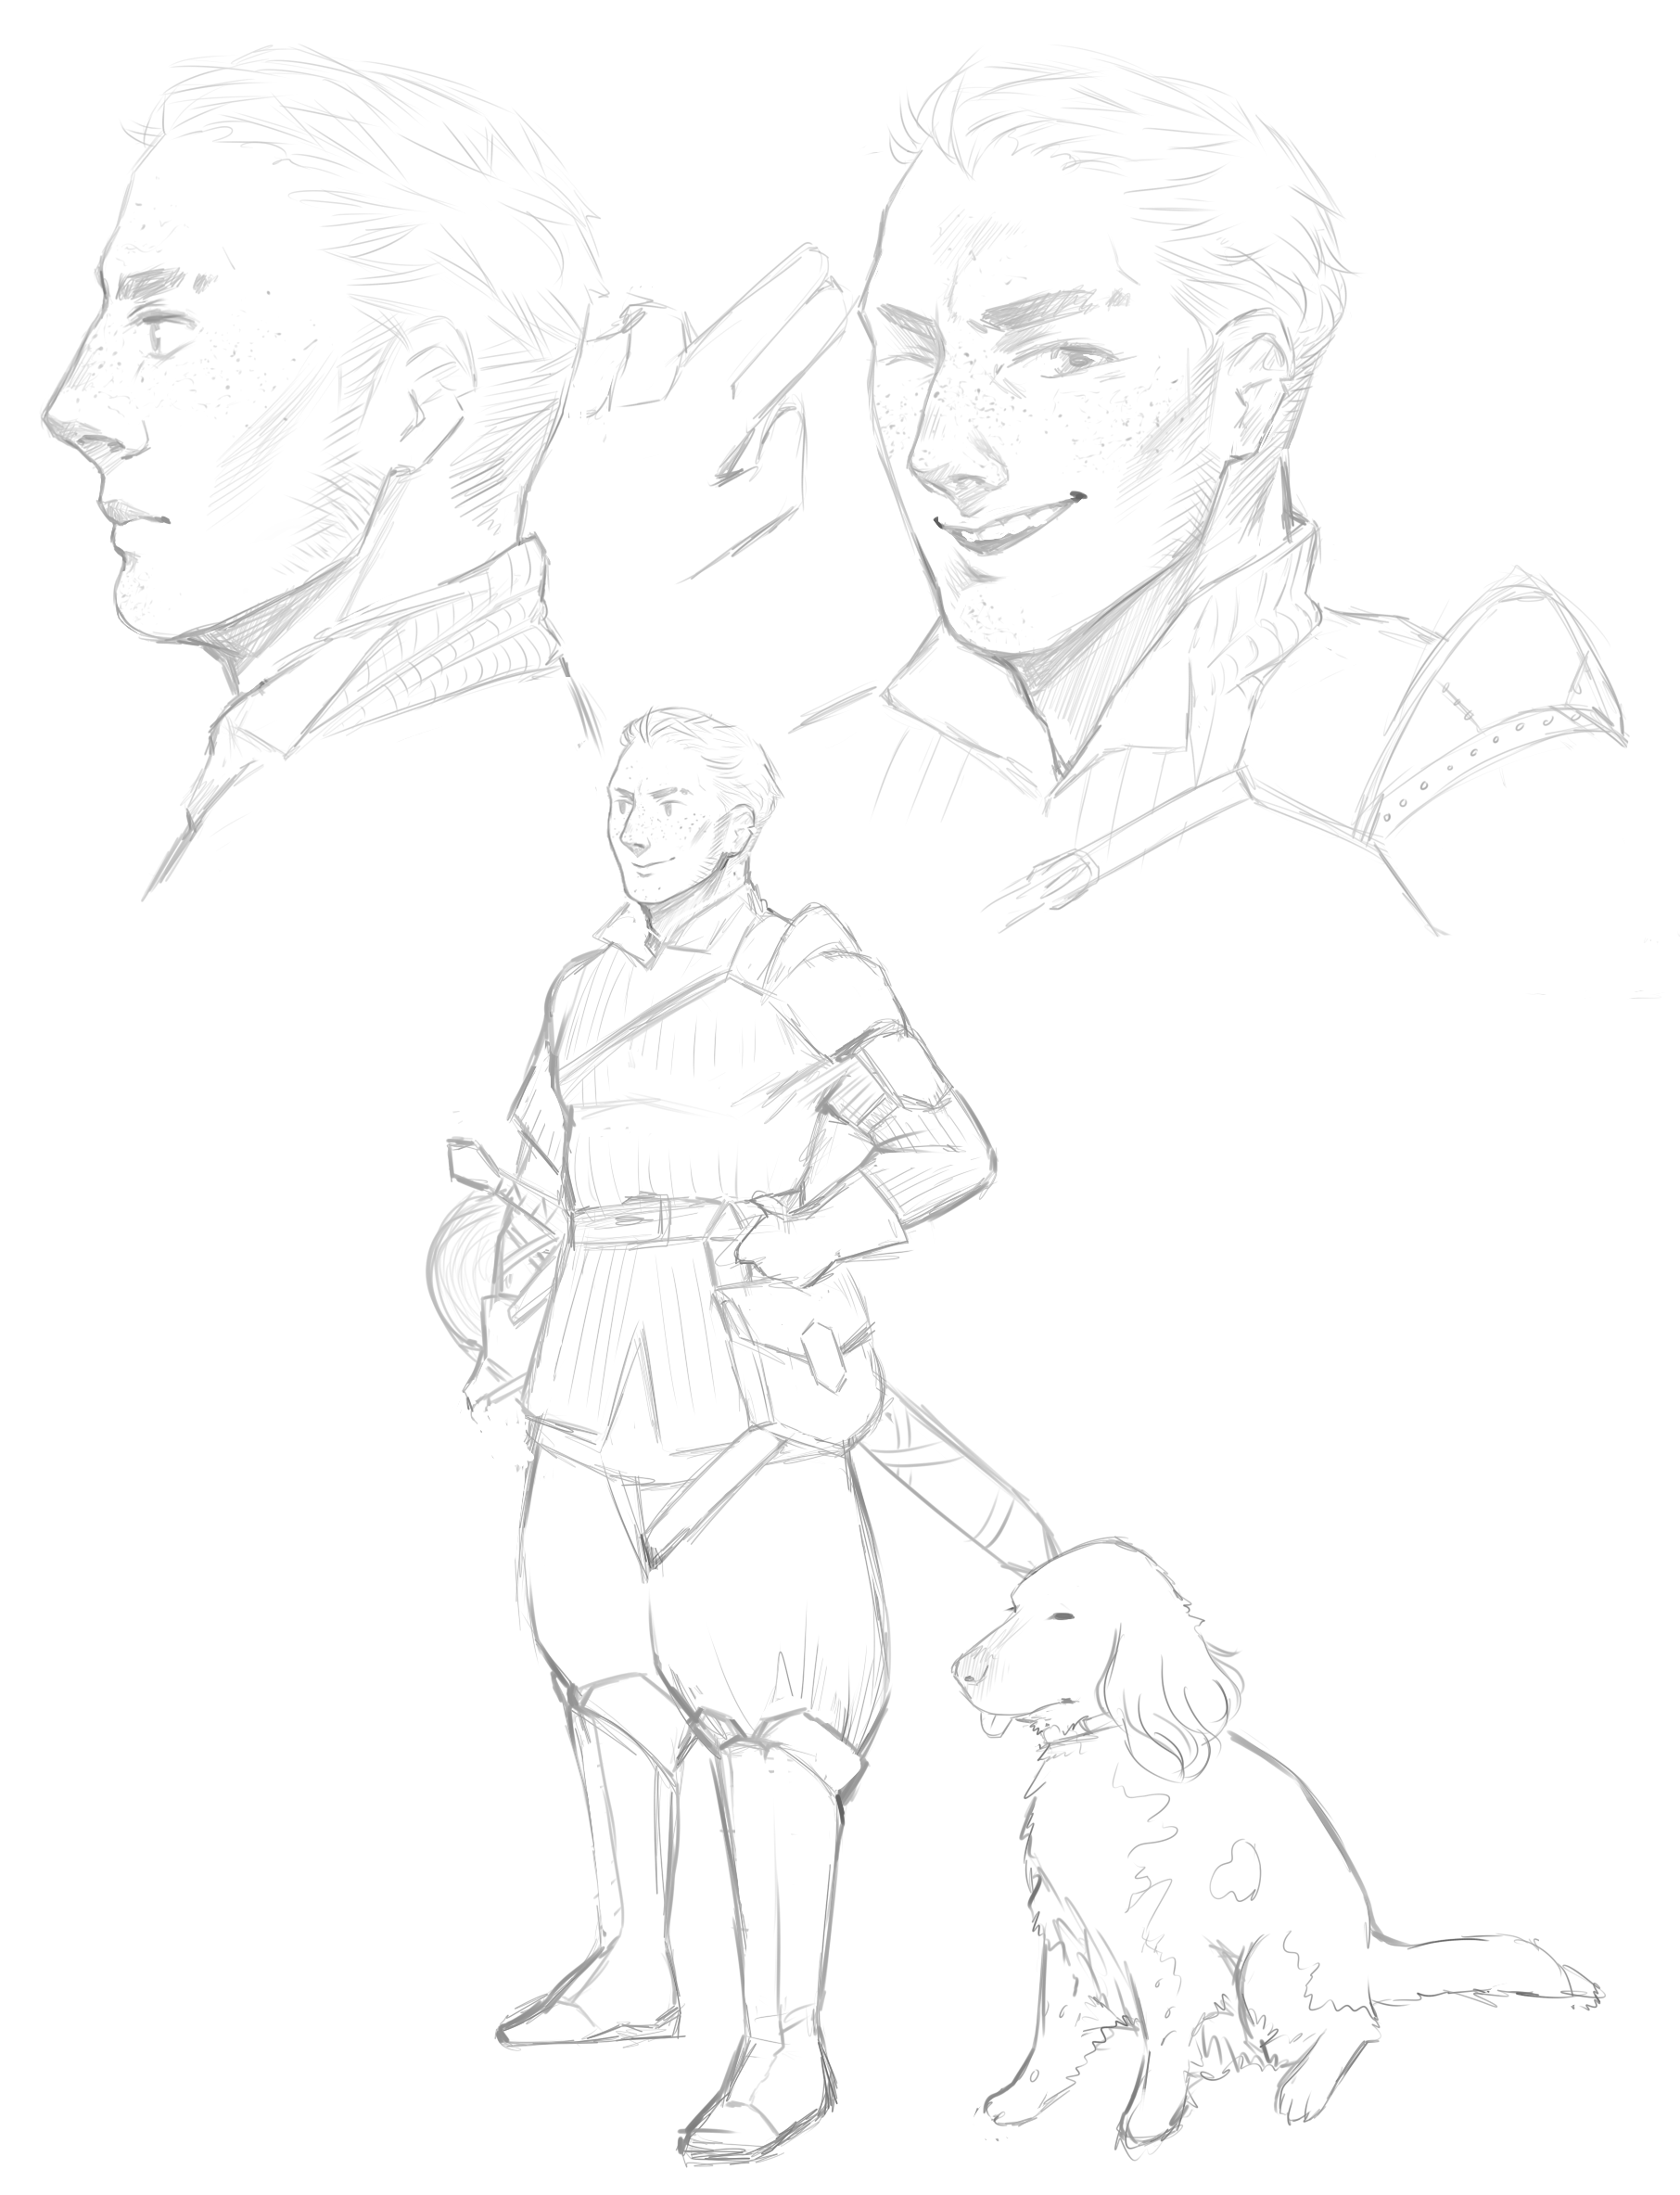
\includegraphics[width=0.75\textheight]{Abbildungen/Abenteuer/Hauptcharaktere/soldat.png}
	\caption[Konzeptart Soldat]{Konzeptart Soldat als 16-Jähriger während dem Hauptteil der Demo.}
	\label{fig:mc_soldat}
\end{figure}

\section{Diplomatin} \label{sec:mc_diplomatin}
\begin{itemize}
	\item weiblich
	\item Alter:\\
	- 17 zur Demo
	\item Aussehen:\\
	- wie dargestellt in Abb. \ref{fig:mc_diplomatin} \\
	- gut gepflegt \\
	- geschminkt
	\item Kleidung:\\
	- legt Wert auf Äußeres\\
	- lange Kleider
	\item Charakter:\\
	- "Mädchen"\\
	- ihr ist die Ehre der Familie sehr wichtig \\
	- legt viel Wert darauf, was andere von ihr halten \\
	- sehr offen gegenüber den schlechter beglückten
	\item Abstammung:\\
	- Mutter: die Geistliche im Amt, eingereist\\
	- Vater: deren Mann, Städter, musste mit seiner Frau mit. Während der Char ein Kind ist, ist er noch sehr unglücklich, später hat er sich mit einigen Männern angefreundet und sich mit der Situation zurechtgefunden. Arbeitet bei einem der innerdörflichen Berufe mit\\
	- Geschwister: mind. 3 offen
	\item Hintergrund:\\
	- absolut gläubig erzogen\\
	- eifert ihrer Mutter darin nach, eine hohe Position im Orden zu erlangen und diesem weiter zu helfen
\end{itemize}

\begin{figure}[h]
	\centering
	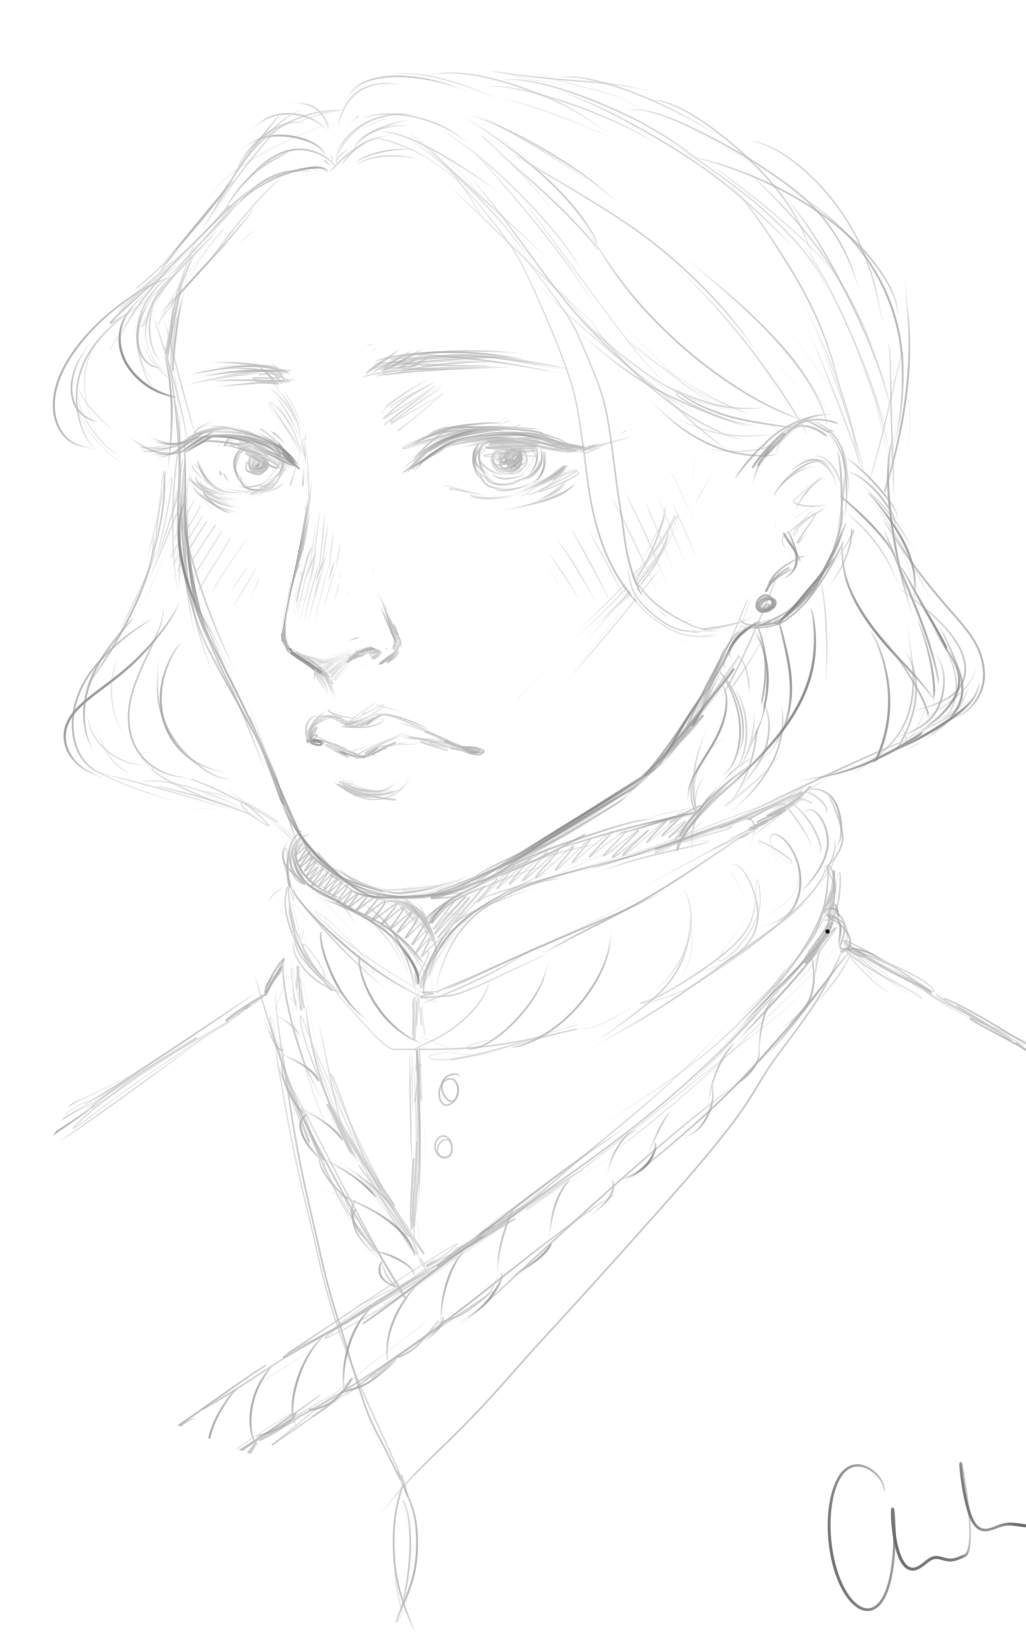
\includegraphics[width=0.325\textheight]{Abbildungen/Abenteuer/Hauptcharaktere/magierin}
	\caption[Konzeptart Diplomatin]{Konzeptart Diplomatin als 17-Jährige während dem Hauptteil der Demo.}
	\label{fig:mc_diplomatin}
\end{figure}


\section{Spionin} \label{sec:mc_spionin}
\begin{itemize}
	\item weiblich
	\item Alter:\\
	- 16 zur Demo
	\item Aussehen:\\
	- wie dargestellt in Abb. \ref{fig:mc_spionin}\\
	- Zopf bis Brust
	\item Kleidung:\\
	- praktisch\\
	- Hosen \\
	- Bogen, Dolch (zum Ausnehmen Wild) am Gürtel\\
	- Gugel?
	\item Charakter:\\
	- praktisch veranlagt\\
	- Wildfang \\
	- zynisch \\
	- schwarzer Humor
	\item Abstammung:\\
	- Vater: Jäger\\
	- Mutter: \\
	- Geschwister: einige offen
	\item Hintergrund:\\
	- arme und ungebildete Familie\\
	- aufgewachsen am Rand des Dorfes oder ggf. am Waldrand bei den 2-3 Jägerhütten
\end{itemize}

\begin{figure}
	\centering
	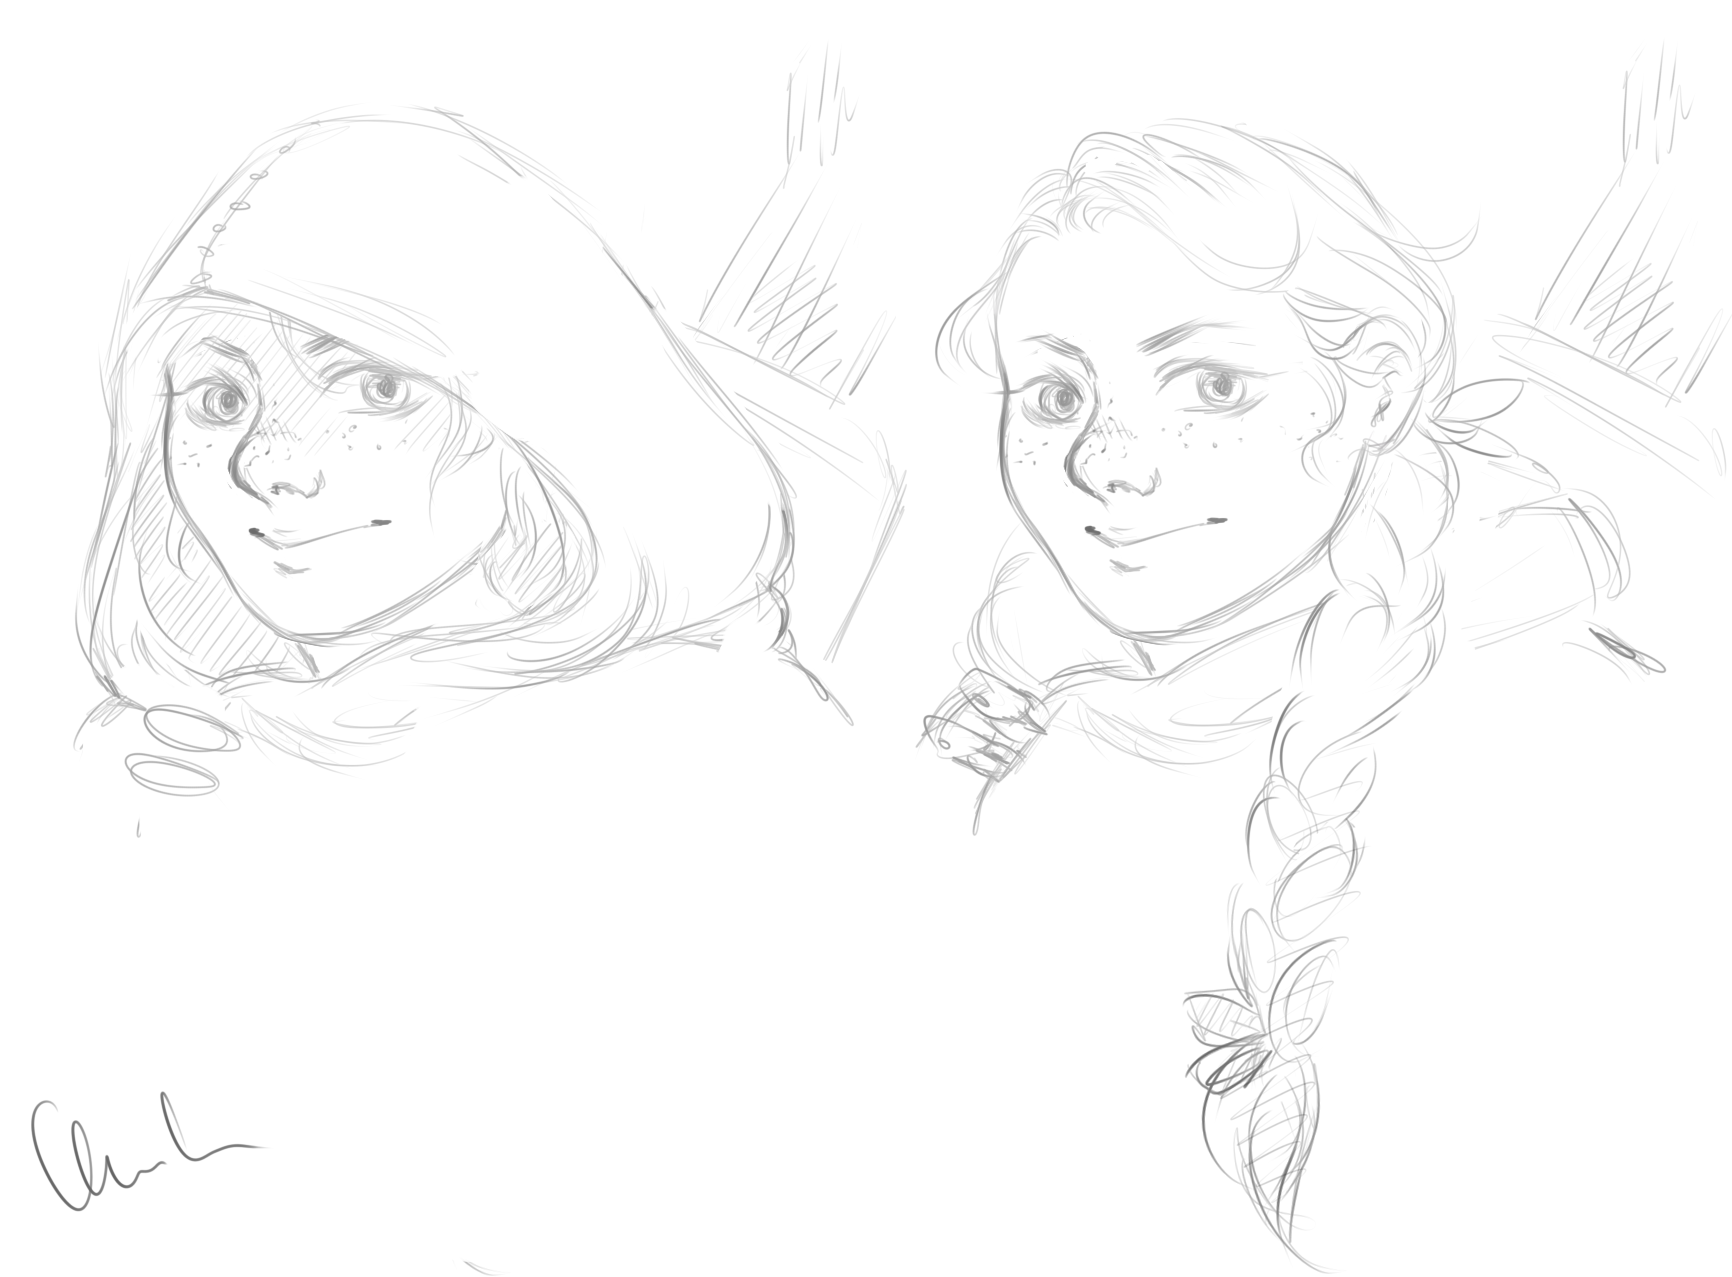
\includegraphics[width=0.9\textwidth]{Abbildungen/Abenteuer/Hauptcharaktere/spionin}
	\caption[Konzeptart Spionin]{Konzeptart Spionin als 16-Jährige während dem Hauptteil der Demo.}
	\label{fig:mc_spionin}
\end{figure}

\chapter{Hauptmission}
\section{Prolog}
Teil der Demo
\begin{itemize}
	\item Quests zur Festlegung der Magieausprägungen des Spielers
	\item Quests zur Erlernung von Fähigkeiten
	\item Lernen der Questarten
\end{itemize}
\section{Kapitel 1: Jugend}
Teil der Demo
\begin{itemize}
	\item Die 3 Abenteurer lernen sich kennen und erleben erste gemeinsame Abenteuer.
\end{itemize}
\section{Kapitel 2: Ausbildung}
Tutorials zu den Fertigkeiten
\section{Kapitel 3: Kampf für den Orden}
erste Quests
\section{Kapitel 4Forschung zur Magie in Gegenständen}
\begin{itemize}
	\item Spieler stößt auf Ritual/Erz wodurch man Gegenstände mit Magie verbinden kann
	\item Zuspitzung der Situation mit den Rebellen
\end{itemize}
\section{Kapitel 5: Erschaffung eines Gottes}
\begin{itemize}
	\item Quests gegen die Rebellen: Entscheidung für Erfüllung oder Missachtung der Aufträge bleibt offen
	\item Erschaffung des Gottes, was das Leben aller in einem näheren Umfeld aussaugt (schnelle Alterung), alle anderen sind ihrer Magie beraubt allerdings wirkt auch keine Magie mehr auf sie
	\item Spieler wird zum Propheten des Gottes
\end{itemize}


\part{Mechaniken}
\chapter{Regeneration}
Bei allen Mechaniken sollte der Fakt bedacht werden, dass wir ein Rollenspiel mit Fokus auf die Geschichte und Entwicklung wollen. Der Kampf soll keine primäre Rolle spielen wie bspw. in Skyrim.

\section{Leben}
\begin{itemize}
	\item der Spieler erhält eine sehr kleine Auto-Regeneration. Die natürliche Selbstheilung. In ruhigen Momenten (z.B. Schlaf) regeneriert er pro Stunde zB 2 Prozent seines maximalen Lebens. So können kleine Kampfwunden auch von alleine heilen.
	\item weitere Möglichkeiten zur Heilung: Das Aufsuchen von Heilern und Essen.
	\item Heiler können einen nach entsprechender Gebühr und in einer Zeitspanne, die abhängig von ihrer Expertise ist, komplett voll heilen
	\item Durch Essen lässt sich maximal 60 Prozent des Effektivschadens am Gesamtleben heilen. Verliert der Spieler mehr als 60 Prozent Leben, dann ist die Verletzung entsprechend intensiv und signifikant und soundso viele Prozentpunkte müssen von einem Heiler behandelt werden (permanenter Schaden bis geheilt).
\end{itemize}

\section{Mana}

\section{Hunger}
\begin{itemize}
	\item Man muss täglich wenigstens einen Happen zu sich nehmen, sonst bekommt man Debuffs (auf höheren Schwierigkeitsstufen mehr zB dreimal täglich ausreichend viel, auf niedrigeren zB gar nichts). Je länger, desto heftiger die Debuffs
	\item Man hat einen vergrößerten, aber nicht überdimensionierten Magen. Das bedeutet: Stopft man viel zu viel Essen in sich hinein, bekommt man ab einer gewissen Schwelle nach den 100 Prozent "Magen voll" (zB bei 150 Prozent) Debuffs, weil man Bauchschmerzen hat. Stopft man dann noch mehr in sich rein (zB bis 200 Prozent), dann muss man sich übergeben und verliert alles, was noch im Magen ist, und nimmt zudem etwas Schaden (durch das heftige Kotzen). Zudem verweigert der Spielercharakter für zB eine Woche das Essen des i-Tüpfelchens (was das Brechen dann ausgelöst hat), weil ihm schon bei dem Gedanken schlecht wird. 
	\item Die Magen-Anzeige im Spiel umfasst natürlich nur 0-100 Prozent
	\item Regeneration durch Essen erfolgt sekündlich immer um den gleichen Betrag (nicht Prozent!) - wie lange wird durch das jeweilige Essen festgelegt. So wird eine Gurke zB nur für 1s heilen, eine Buttercremetorte oder ein Fasanenbraten hingegen für 30s. Den Magen füllen sie ebenso unterschiedlich. 
	\item Idee für Erweiterung des Soldaten-Regenerationsskills: ein Punkt kann sein, dass er gelernt hat, sein Essen bedachter zu verspeisen und besser zu verwerten. Das führt zu einer Erhöhung der Heilung pro Sekunde
	\item Idee: jeder/einer/zwei der Start-Charas könnte eine Unverträglichkeit bzw "schmeckt nicht" haben. Das führt dazu, dass man mit diesem Chara dieses Essen nicht nutzen kann bzw. im zweiten Fall dieses Essen nur einen minimalen Bruchteil der Regeneration bietet. Und zB nach einer gewissen Menge, die man das in sich stopft (unabhängig vom 150 Prozent Magen), dann auch Debuffs dazu kommen\\
	man kann das natürlich festschreiben oder wir lassen den Spieler am Anfang des Spiels selbst entscheiden, was es wird, indem das ein Teil einer Kinder-Quest ist
\end{itemize}
\chapter{Leveling und Skills}
\section{Leveling}
\begin{itemize}
	\item Es gibt verschiedene Arten von Skills. Manche können erlernt und etwas gesteigert werden, ohne dass dafür besondere Dinge oder Zeit nötig sind (zB Regeneration). Die anderen wiederum haben ein bestimmtes System aus Selbst-Lernen, Lehrmeistern und Üben
	\item Ich erkläre das System am Beispiel des Schlösserknackens unter der Annahme, dass wir 5 Stufen der Beherrschung eines Skills einführen (zB Neuling, Lehrling, Adept, Meister, Großmeister)
	\item Zu Beginn hat man die Fähigkeit nicht. Es gibt nun zwei Wege, sie zu erwerben:\\
	1. Selbstlehrend. Dabei setzt man sich einfach mal an ein zu knackendes Schloss und egal ob man es schafft oder nicht, man ist nun in der ersten Stufe, Neuling. \\
	2. Lehrmeister. Man kann auch zu einem entsprechenden Lehrmeister gehen (z.B. ein Schlosser) und ihn bitten, einem die Grundlagen beizubringen.
	\item um nun die Fähigkeit zu verbessern sind zwei Abschnitte relevant: Das Üben und der Aufstieg in die nächste Stufe (und damit verbunden neue Fähigkeiten-Möglichkeiten)
	\item erstmal zum Aufstieg. Um die nächste Stufe zu erreichen, ist IMMER ein Lehrmeister (oder auf den niedrigen Stufen meinetwegen auch Lehrbücher) nötig. Dies sorgt auch dafür, dass wir die Relevanz von Geld in unserem Spiel erhöhen.
	In unserem Beispiel würde einem der Schlosser Erläuterungen zu kompizierteren Schlössern geben und sie zeigen.
	\item das Üben ist nötig, bevor man aufsteigen darf. Denn nur, weil ich die Grundschule geschafft habe, heißt das nicht, dass ich bereit für den Master bin. Keiner kann als Kind direkt nach der Erklärung zum Fahrradfahren losradeln und fährt nicht in den nächsten Baum oder kippt um.
	Üben beideutet die Anwendung des Skills in Ausreichender Menge oder Zeit für das Erreichen der kommenden Stufe. Das muss im Allgemeinen während des Spiels erfolgen. Allerdings können da die Lehrmeister - eingeschränkt - helfen. So könnte einem der Schlosser ein paar alte oder falsche oder einfach Übungsschlösser zur Verfügung stellen, damit man an ihnen üben kann. Das kostet natürlich. Macht man dieses Üben unter Aufsicht eines Meisters, dann kommt man schneller voran (man muss zB nicht 20 sondern nur 10 Schlösser knacken). ABER die Menge der Übung, die man bei einem Meister absolvieren kann, variiert je nach aktueller Stufe. So kann man im niedrigsten Bereich alle Übungseinheiten beim Meister absolvieren, doch will man Großmeister werden, dann vllt nur die ersten 20 Prozent...
	\item andere Skills wiederum gibt es nur in einer Steigerungsform: Man kann sie oder auch nicht und vielleicht kann man besser werden, aber nur in einem marginalen Rahmen und dann nur durch Anwendung (zB tanzen)
\end{itemize}

\section{Skills}
\begin{itemize}
	\item Idee für Erweiterung des Soldaten-Regenerationsskills: ein Punkt kann sein, dass er gelernt hat, sein Essen bedachter zu verspeisen und besser zu verwerten. Das führt zu einer Erhöhung der Heilung pro Sekunde
\end{itemize}

\section{Quest-Belohnungen}
\begin{itemize}
	\item viele der optionalen Quests sollen abhängig von ihrer Beschaffenheit dem Spieler wirklich auch eine tolle Belohnung geben: mehr Leben und "mehr" Mana und Resistenzen. Da wir keine Gegenstände haben, in die man solches mittels Verzauberungen legen könnte, ist das eine schöne Möglichkeit, sie dem Spieler trotzdem zur Verfügung zu stellen und ihn damit stärker werden zu lassen
	\item  blöd gesagt: wenn ich eine stinknormale Banditenbande ausnehme, habe ich ja Wunden erfahren, also weiß ich wieder besser mit meinen körpereigenen Regenerationskräften umzugehen und habe ab dann eine leicht erhöhte Regeneration (anstatt 2 Prozent pro h während Rasten oder Schlafen halt 2,5 Prozent oder so). Oder wenn ich in der Quest einem Alchemisten der Uni bei der Mischung und oder dem Ausprobieren eines Trankes helfen soll, steigt meine Resistenz ggü. Giften oder so was. Oder weil ich bei der Banditenbande oben ja gegen die gekämpft habe, habe ich nun mehr Erfahrung im kleinen Ausweichen, weshalb ich es schaffe, häufig weniger Schaden zu nehmen, aka mein Leben erhöht sich etc
	\item  die Rewards normaler Nebenquests sind in der Regel festgelegt von ihrem Wert und ihrer Stufe (bei Waffen und Rüstung). Denn der Bauer wird dir egal wie mächtig du bist, immer nur das gleiche bieten können als Bezahlung. Die Hauptquest, die der Spieler ja auch aktiv erstmal warten lassen soll, um die Nebenquests zu erkunden und zu machen,  wird mitleveln, damit es nicht wie in vielen Spielen ist, dass man sich erstmal an Nebenquests hocharbeitet und die HQ danach nur noch durchrennen und Oneshotten ist und man die Belohnung "das mächtige Schwert des Weisen" direkt zerstört, weil man keinen Platz im Inventar hat, es aber mittlerweile 20 Stufen später weniger wert ist, als der Rest im Rucksack...
\end{itemize}
\chapter{Nutzung der Karte(n)}
\begin{itemize}
	\item Ingame-Map die der Spieler per Tastendruck aufrufen kann
	\item Per Tastendruck (Standard 'M') öffnet sich die Map der Spielewelt. Der Spielercharakter wird als kleines 3D-Figürchen dargestellt
	\item Besuchte Bereiche der Spielwelt werden normal angezeigt
	\item Bereiche die der Spieler noch nicht besucht hat werden durch schwarzen "Rauch" verdeckt
	\item Für Leute, die es nur auf die Story und weniger auf das Erkunden der Welt abgesehen haben, könnte man den Spieler mit seinem Miniatur-Figürchen interagieren lassen - Der Spieler könnte quasi das Figürchen über bereits aufgedeckte Straßen (NUR aufgedeckte Bereiche) ziehen um "Quicktravel" zu simulieren
	\item Eventuell lässt man dann die Ingame-Zeit schneller verstreichen während man diese Mechanic benutzt
	\item Quicktravel sollte nur von vorbestimmten Punkten zu bestimmten Punkten erlaubt sein. Zum Beispiel ein Kutschensystem zwischen den wichtigsten Orten.
\end{itemize}
\chapter{Speichern}
\begin{itemize}
	\item keine Quicksaves, denn: trag gefälligst die Konsequenzen deiner Entscheidung und lad nicht neu, bis es dir gefällt
	\item Autosaves an relevanten Punkten wie zB direkt vor bestimmten Kämpfen etc und IMMER direkt nach Spielrelevanten Entscheidungen
	\item wenn man absichtlich Speichern will ähnlich wie bei KCD: Spezieller Einmal-Save beim Beenden, immer möglich bei bestimmten sozialen Interaktionen oder an besonderen Orten oder so und bestimmtes Item, mit dem man Speichern kann.
	\item Funktionsweise des Einmal-Save: Das angelegte Savegame, wird beim Laden/erneuten Spielbeginn wieder gelöscht. Es kann also nur einmal verwendet werden und ist kein dauerhafter Speicherstand\\
	D.h. man kann immer und überall speichern, aber nur wenn man das Spiel wirklich verlässt.
\end{itemize}

%----------Anhänge------------


\end{document}